% Todo lo que considero como ejemplo proviene de tesis de ejemplo para el grado de ingeniero del MIT.

%%%%%%%%%%%%%%%%%%%%%%%%%%%%%%%%%%%%%%%%%
% Masters/Doctoral Thesis
% LaTeX Template
% Version 2.3 (25/3/16)
%
% This template has been downloaded from:
% http://www.LaTeXTemplates.com
%
% Version 2.x major modifications by:
% Vel (vel@latextemplates.com)
%
% This template is based on a template by:
% Steve Gunn (http://users.ecs.soton.ac.uk/srg/softwaretools/document/templates/)
% Sunil Patel (http://www.sunilpatel.co.uk/thesis-template/)
%
% Template license:
% CC BY-NC-SA 3.0 (http://creativecommons.org/licenses/by-nc-sa/3.0/)
%
%%%%%%%%%%%%%%%%%%%%%%%%%%%%%%%%%%%%%%%%%

%----------------------------------------------------------------------------------------
%	PACKAGES AND OTHER DOCUMENT CONFIGURATIONS
%----------------------------------------------------------------------------------------

\documentclass[
11pt, % The default document font size, options: 10pt, 11pt, 12pt
%oneside, % Two side (alternating margins) for binding by default, uncomment to switch to one side
%chapterinoneline,% Have the chapter title next to the number in one single line
english, % ngerman for German
spanish,
singlespacing, % Single line spacing, alternatives: onehalfspacing or doublespacing
%draft, % Uncomment to enable draft mode (no pictures, no links, overfull hboxes indicated)
%nolistspacing, % If the document is onehalfspacing or doublespacing, uncomment this to set spacing in lists to single
liststotoc, % Uncomment to add the list of figures/tables/etc to the table of contents
%toctotoc, % Uncomment to add the main table of contents to the table of contents
parskip, % Uncomment to add space between paragraphs
%nohyperref, % Uncomment to not load the hyperref package
headsepline, % Uncomment to get a line under the header
]{MastersDoctoralThesis} % The class file specifying the document structure

\usepackage{mathtools}% http://ctan.org/pkg/mathtools
\usepackage[utf8]{inputenc} % Required for inputting international characters
\usepackage[T1]{fontenc} % Output font encoding for international characters
\usepackage{palatino} % Use the Palatino font by default
\usepackage{float} % Para ubicar imagenes en donde corresponden
\usepackage{flexisym}
\usepackage[table]{xcolor}% http://ctan.org/pkg/xcolor
\usepackage{booktabs}

% \usepackage{indentfirst}
% \setlength\parskip{.5\baselineskip plus .1\baselineskip  minus .1\baselineskip}
% \setlength{\parindent}{1em}

\setlength{\parindent}{0.5cm}

\usepackage[ddmmyyyy]{datetime}

\usepackage{titlesec}
\setcounter{secnumdepth}{4}
\titleformat{\paragraph}{\normalfont\normalsize\bfseries}{\theparagraph}{1em}{}
\titlespacing*{\paragraph}{0pt}{3.25ex plus 1ex minus .2ex}{1.5ex plus .2ex}

\usepackage{caption}
\captionsetup[table]{name=Tabla}
\captionsetup[figure]{name=Figura}

\usepackage[backend=bibtex,style=numeric,maxcitenames=1,natbib=true,sorting=none]{biblatex}
\addbibresource{references.bib} % The filename of the bibliography
\usepackage[autostyle=true]{csquotes} % Required to generate language-dependent quotes in the bibliography

\DefineBibliographyStrings{spanish}{%
  andothers = {et\addabbrvspace al\adddot}
}

\usepackage{amsmath}
\usepackage{amssymb}
\usepackage{graphicx}

% Paquetes para las tablas
\usepackage{tablefootnote}

% Paquete para Gantt
\usepackage{pgfgantt}


% BULLET a DASH
\usepackage{enumitem}
\setlist[itemize]{label=$-$}

%----------------------------------------------------------------------------------------
%	MARGIN SETTINGS
%----------------------------------------------------------------------------------------

\geometry{
	paper=a4paper, % Change to letterpaper for US letter
	inner=2.5cm, % Inner margin
	outer=3.8cm, % Outer margin
	bindingoffset=2cm, % Binding offset
	top=1.5cm, % Top margin
	bottom=1.5cm, % Bottom margin
	%showframe,% show how the type block is set on the page
}

%----------------------------------------------------------------------------------------
%	THESIS INFORMATION
%----------------------------------------------------------------------------------------

\thesistitle{Desarrollo de un sistema de gestión de programas de estudio orientado a resultados pedagógicos} % Your thesis title, this is used in the title and abstract, print it elsewhere with \ttitle
\supervisor{Ing. Sebastián \textsc{Ortíz} \\ Ing. Wilfrido \textsc{Inchaustti}} % Your supervisor's name, this is used in the title page, print it elsewhere with \supname
\examiner{} % Your examiner's name, this is not currently used anywhere in the template, print it elsewhere with \examname
\degree{Ingeniería Informática} % Your degree name, this is used in the title page and abstract, print it elsewhere with \degreename
\author{Luis F. \textsc{Villalba V.}} % Your name, this is used in the title page and abstract, print it elsewhere with \authorname
\addresses{} % Your address, this is not currently used anywhere in the template, print it elsewhere with \addressname

\subject{Desarrollo ágil} % Your subject area, this is not currently used anywhere in the template, print it elsewhere with \subjectname
\keywords{agile, development, ams, cms, competencias, diseño, curriculum, desarrollo, observación, participante, caso, estudio} % Keywords for your thesis, this is not currently used anywhere in the template, print it elsewhere with \keywordnames
\university{\href{http://www.universidadcatolica.edu.py/}{Universidad Católica "Nuestra Señora de la Asunción"}} % Your university's name and URL, this is used in the title page and abstract, print it elsewhere with \univname
\department{\href{http://www.dei.uc.edu.py/}{Departamento de Electrónica e Informática}} % Your department's name and URL, this is used in the title page and abstract, print it elsewhere with \deptname
\faculty{\href{http://www.cyt.uc.edu.py/}{Facultad de Ciencias y Tecnología}} % Your faculty's name and URL, this is used in the title page and abstract, print it elsewhere with \facname

\hypersetup{pdftitle=\ttitle} % Set the PDF's title to your title
\hypersetup{pdfauthor=\authorname} % Set the PDF's author to your name
\hypersetup{pdfkeywords=\keywordnames} % Set the PDF's keywords to your keywords
\hypersetup{
    colorlinks = blue,
    filecolor = magenta,
    linkcolor = blue,		% Links del indice, etc
    urlcolor = blue,		% Links de texto con URL asociado
    citecolor = blue,		% Links de texto citado
}

\begin{document}

\frontmatter % Use roman page numbering style (i, ii, iii, iv...) for the pre-content pages
\pagestyle{plain} % Default to the plain heading style until the thesis style is called for the body content

%----------------------------------------------------------------------------------------
%	COVER PAGE
%----------------------------------------------------------------------------------------

\begin{titlepage}
\begin{center}

\begin{figure}[H]
\centering

\includegraphics{Figuras/uca}
\decoRule
%\caption[Logo de la UCA]{UCA.}
\end{figure}

{\scshape\LARGE \univname\par}\vspace{1.5cm} % University name
\textsc{\Large Proyecto final de carrera}\\[0.5cm] % Thesis type

\HRule \\[0.4cm] % Horizontal line
{\huge \bfseries \ttitle\par}\vspace{0.4cm} % Thesis title
\HRule \\[1cm] % Horizontal line

\Large \emph{Autor:}\\
\Large \href{}{\authorname} \\[5mm] % Author name - remove the \href bracket to remove the link
\Large \emph{Tutores:}\\
\Large \href{}{Ing. Sebastián \textsc{Ortíz} \\ Ing. Wilfrido \textsc{Inchaustti}} \\[1cm]

\Large \facname\\ % Research group name and department name
\Large \deptname \\[5mm]

{\large\the\year}\\[1cm] % Date

\end{center}
\end{titlepage}


%----------------------------------------------------------------------------------------
%	TITLE PAGE
%----------------------------------------------------------------------------------------

\begin{titlepage}
\begin{center}
\vspace*{3cm}

{\huge \ttitle\par}\vspace{1cm} % Thesis title
\HRule \\[2cm] % Horizontal line

\begin{minipage}[t]{0.4\textwidth}
\begin{flushleft} \large
\emph{Autor:}\\
\href{}{\authorname} % Author name - remove the \href bracket to remove the link
\end{flushleft}
\end{minipage}
\begin{minipage}[t]{0.4\textwidth}
\begin{flushright} \large
\emph{Tutores:} \\
\href{}{\supname} % Supervisor name - remove the \href bracket to remove the link
\end{flushright}
\end{minipage}\\[2cm]

\large \textit{Una tesis presentada en cumplimiento de los requisitos\\ para el título de \degreename \ en la}\\[1cm]

\univname\\ % University name
\facname\\ % Research group name and department name
\deptname \\[2cm]

{\large\today}\\[1cm] % Date

\vfill

\end{center}
\end{titlepage}


%----------------------------------------------------------------------------------------
%	DECLARATION PAGE
%----------------------------------------------------------------------------------------

\renewcommand{\authorshipname}{Declaración de autoría}

\begin{declaration}
\addchaptertocentry{\authorshipname}

\noindent Yo, \authorname, declaro que la tesis titulada, \enquote{\ttitle} y todo el trabajo presentado son de mi propiedad. Además, confirmo que:

\begin{itemize}
\item Este trabajo fue llevado a cabo bajo las normas y regulaciones del Reglamento De Proyecto Final de Carrera (09/2015) del Departamento de Ingeniería Electrónica e Informática.
\item Este trabajo fue realizado en su totalidad con fines investigativos y para obtener el título antes mencionado en esta universidad.
\item Cuando cualquier parte de esta tesis haya sido previamente sometida a un título en esta universidad o cualquier otra institución, esto se ha manifestado claramente.
\item Donde he consultado trabajo publicado por otros autores, eso ha sido siempre claramente atribuido.
\item Donde he citado trabajo de otros autores, la fuente siempre se ha dado. Con la excepción de dichas citas, esta tesis es enteramente mi propio trabajo.
\item He reconocido todas las fuentes principales de ayuda.
\item Donde la tesis está basada en mi trabajo en conjunto con otros autores, he expresado claramente que fue hecho por ellos y en que he contribuido.\\
\end{itemize}

\noindent Firma:\\
\rule[0.5em]{25em}{0.5pt} % This prints a line for the signature

\noindent Fecha:\\
\rule[0.5em]{25em}{0.5pt} % This prints a line to write the date
\end{declaration}

\cleardoublepage

%----------------------------------------------------------------------------------------
%	QUOTATION PAGE	solo si es necesario
%----------------------------------------------------------------------------------------

%\vspace*{0.2\textheight}

%\noindent\enquote{\itshape Thanks to my solid academic training, today I can write hundreds of words on virtually any topic without possessing a shred of information, which is how I got a good job in journalism.}\bigbreak

%\hfill Dave Barry

%----------------------------------------------------------------------------------------
%	ABSTRACT PAGE
%----------------------------------------------------------------------------------------

\renewcommand{\abstractname}{Abstract}

\begin{abstract}
\addchaptertocentry{\abstractname} % Add the abstract to the table of contents



\end{abstract}

%----------------------------------------------------------------------------------------
%	ACKNOWLEDGEMENTS
%----------------------------------------------------------------------------------------

\renewcommand{\acknowledgementname}{Agradecimientos}

\begin{acknowledgements}
\addchaptertocentry{\acknowledgementname} % Add the acknowledgements to the table of contents

%  Se escribe en primera persona. Se agradece a la universidad por impartir los conocimientos, al tutor, al co-tutor, a la mesa de tesis, a todas las personas que influyeron o colaboraron de alguna forma en el proyeto, Paz, padres, hermanos, familia, amigos de la facultad, compañeros de trabajo, compañeros de colegio, trankas, etc.
The acknowledgments and the people to thank go here, don't forget to include your project advisor\ldots

\end{acknowledgements}

%----------------------------------------------------------------------------------------
%	LIST OF CONTENTS/FIGURES/TABLES PAGES
%----------------------------------------------------------------------------------------

\renewcommand{\contentsname}{Índice General}
\tableofcontents % Prints the main table of contents

\renewcommand{\listfigurename}{Lista de Figuras}
\listoffigures % Prints the list of figures

\renewcommand{\listtablename}{Lista de Tablas}
\listoftables % Prints the list of tables

%----------------------------------------------------------------------------------------
%	ABBREVIATIONS
%----------------------------------------------------------------------------------------

\begin{abbreviations}{ll} % Include a list of abbreviations (a table of two columns)

\textbf{AMS} & \textbf{A}ssessment \textbf{M}anagement \textbf{S}ystem\\
\textbf{CMS} & \textbf{C}urriculum \textbf{M}anagement \textbf{S}ystem \\
\textbf{UX} & \textbf{U}ser e\textbf{X}perience \\
\textbf{LMS} & \textbf{L}earning \textbf{M}anagement \textbf{S}ystem \\
\textbf{SaaS} & \textbf{S}oftware \textbf{a}s \textbf{a} \textbf{S}ervice \\
\textbf{SLO} & \textbf{S}tudent \textbf{L}earning \textbf{O}utcomes \\
\textbf{PCAH} & \textbf{P}rogram and \textbf{C}ourse \textbf{A}pproval \textbf{H}andbook \\
\textbf{INVEST} & e\textbf{I}ndependent \textbf{N}egotiable \textbf{V}aluable \textbf{E}stimatable \textbf{S}mall \textbf{T}estable \\
\textbf{HCI} & \textbf{H}uman \textbf{C}omputer \textbf{I}nteraction \\
\textbf{UI} & \textbf{U}ser \textbf{I}nteraction \\
\textbf{DECA} & \textbf{DE}cision a\textbf{CA}demic \\
\textbf{AWS} & \textbf{A}mazon \textbf{W}eb \textbf{S}ervices \\
\textbf{VCS} & \textbf{V}ersion \textbf{C}ontrol \textbf{S}ystem \\
\textbf{MVC} & \textbf{M}odel \textbf{V}iew \textbf{C}ontroller \\
\textbf{UI} & \textbf{U}ser \textbf{I}nteraction \\
\textbf{POJO} & \textbf{P}lain \textbf{O}ld \textbf{J}ava \textbf{O}bject \\

\end{abbreviations}

%----------------------------------------------------------------------------------------
%	PHYSICAL CONSTANTS/OTHER DEFINITIONS
%----------------------------------------------------------------------------------------

%\begin{constants}{lr@{${}={}$}l} % The list of physical constants is a three column table

% The \SI{}{} command is provided by the siunitx package, see its documentation for instructions on how to use it

	%Speed of Light & $c_{0}$ & \SI{2.99792458e8}{\meter\per\second} (exact)\\
%Constant Name & $Symbol$ & $Constant Value$ with units\\

%\end{constants}

%----------------------------------------------------------------------------------------
%	SYMBOLS
%----------------------------------------------------------------------------------------

%\begin{symbols}{lll} % Include a list of Symbols (a three column table)

%$a$ & distance & \si{\meter} \\
%$P$ & power & \si{\watt} (\si{\joule\per\second}) \\
%Symbol & Name & Unit \\

%\addlinespace % Gap to separate the Roman symbols from the Greek

%$\omega$ & angular frequency & \si{\radian} \\

%\end{symbols}

%----------------------------------------------------------------------------------------
%	DEDICATION   solo si es necesario
%----------------------------------------------------------------------------------------

%\dedicatory{ Dedicado a\ldots}
% For/Dedicated to/To my

%----------------------------------------------------------------------------------------
%	THESIS CONTENT - CHAPTERS
%----------------------------------------------------------------------------------------

\mainmatter % Begin numeric (1,2,3...) page numbering

\pagestyle{thesis} % Return the page headers back to the "thesis" style

% Include the chapters of the thesis as separate files from the Chapters folder
\renewcommand{\chaptername}{Capítulo}
\newcommand{\ra}[1]{\renewcommand{\arraystretch}{#1}}

% INTRODUCCION
\chapter{Introducción}
\section{Justificación}
Existe un consenso, tanto entre los empleadores como los funcionarios de gobierno, de que en los Estados Unidos se necesita un mayor número de estudiantes en nivel técnico y universitario que posean habilidades comprobadas\citep{kuh_knowing_2014}. Esto ha llevado a una gran presión sobre las instituciones educativas para que provean más y mejor evidencia de los logros del proceso educativo\citep{kuh_knowing_2014}. Para intentar llenar este vacío se ha creado la evaluación basada en competencias, la cual se enfoca en valorar las habilidades adquiridas por un estudiante en el proceso de un programa educativo\citep{cartwright2009student}.
 
De esta manera, las aplicaciones de evaluación académica basadas en competencias han adquirido mucha importancia en los últimos años\citep{barrio_minton_evaluating_2016}. En dichas aplicaciones se busca conocer información acerca de las fortalezas y debilidades del estudiante de una manera modular, en contraposición a los métodos cuantitativos de evaluación. Dichos aprendizajes y competencias son expresados por segmentos de estudios o actividades, mediante resultados esperados medibles a nivel institucional, de programa, grado, o de curso; expresados en calificaciones asociadas a habilidades específicas y no a módulos o cursos de un programa de estudio\citep{kuh_using_2015}. 
 
Para poder realizar una evaluación basada en competencias de un programa educativo, el mismo programa tiene que estar diseñado con esta perspectiva educativa: los programas de estudio e incluso los mismos cursos que lo conforman, tienen que estar diseñados con una perspectiva de orientación a competencias\citep{lalor_ensuring_2017}. La creación de un programa de estudio es una tarea colaborativa que involucra a un gran número de personas que proponen el diseño curricular, los cursos, los resultados esperados del programa. Cada uno de estos elementos debe pasar por un proceso iterativo de creación, revisión y aprobación que involucra a varios funcionarios, autoridades y profesores de las instituciones involucradas\citep{boyle_curriculum_2016}. 
 
En el ámbito de las aplicaciones académicas, si bien existen aplicaciones que abarcan el diseño y la publicación de planes de estudio por parte de los profesores o encargados de las universidades, además de su revisión y posterior aprobación por el comité curricular, no se ha encontrado durante el proceso de relevamiento de herramientas existentes una aplicación que integre todos estos elementos en un sistema de gestión de evaluaciones basadas en competencias\citep{curricunet_webpage}\citep{courseleaf_webpage}\citep{deca_webpage}.
 
En este caso de estudio\citep{runeson2012case} planteamos la posibilidad de crear un sistema de gestión de programas de estudio orientado a resultados pedagógicos y exploramos los desafíos tanto técnicos como de interacción humano computador asociados a dicho desarrollo.
\section{Objetivos}

\subsection{Objetivo general}
Diseñar una aplicación que permita integrar y estructurar tareas separadas de un sistema académico para una gestión de programas educativos orientados a resultados pedagógicos, que provea soporte a flujos de trabajo para sus diferentes etapas de aprobación.


\subsection{Objetivos específicos}
  \begin{itemize}
    \item Realizar un relevamiento de los requerimientos y comparación de las herramientas existentes que aborden la problemática planteada.
    \item Realizar el proyecto en un marco de programación ágil, estimando y desarrollando la aplicación de acuerdo a las directrices brindadas por esta metodología.
    \item Validar la herramienta desarrollada con expertos del dominio principalmente y de manera preliminar con experiencias limitadas con los usuarios finales.
  \end{itemize}
\section{Diseño de la investigación}
El presente trabajo ilustra como caso de estudio la aplicación de la metodología ágil en la gestión de un proyecto de desarrollo de un módulo, integrado a un sistema de gestión y evaluación de competencias de una organización ubicada en los Estados Unidos. El trabajo a realizar fue propuesto por la organización que brinda el sistema de gestión de competencias, donde el mismo sirve como base al módulo de gestión curricular a desarrollarse.

El caso refleja de manera práctica como debería operar un ambiente de desarrollo ágil y de la interrelación entre usuarios ubicados en diferentes localidades como parte del sistema de trabajo. En este proyecto los miembros ubicados en forma remota se encargan del diseño de las tareas, aquí llamadas historias de usuario, a realizarse, y de la validación de las características entregadas.

Debido a que los requisitos de la aplicación a desarrollarse se irán esclareciendo acorde se vayan completando cada valor de negocio, se optó por la metodología ágil como técnica de gestión de desarrollo de software, puesto que es el enfoque más adecuado para poder encarar esta problemática.

La observación participante de parte del investigador es un paso inicial para el desarrollo del sistema en un nuevo equipo, donde se identifican y guían las relaciones con los informantes, lo ayuda a sentir la organización del equipo y las prioridades de desarrollo. También, lo permite integrarse con los demás miembros del mismo y de esa manera le facilita el proceso de investigación, además de proveerle una cantidad de interrogantes a ser dilucidadas con los participantes\citep{erlandson_doing_1993}.

El primer paso es adaptarse a los cambios y a la metodología de trabajo del equipo de desarrollo. Dicho equipo se constituirá luego de a una encuesta previa de capacidades de todos los desarrolladores de la empresa, donde cada uno colocará sus conocimientos en herramientas o en partes del sistema de gestión de competencias, para así poder aprovechar las virtudes de cada persona. Acto seguido se procede al análisis de las herramientas a utilizarse para corroborar que cumplen con las exigencias del sistema a desarrollarse.

Entre algunas técnicas de recolección de información se utilizan las encuestas\citep{robson_real_2011}. Para este sistema un equipo en Estados Unidos utilizó la misma para proporcionar una visión general del área a ser investigada. 

Los casos de estudios con enfoque HCI\footnote{de sus siglas en inglés, Human-Computer Interaction, que significa en español interacción humano-computador.} tienen como meta la comprensión de problemas o situaciones mediante la interacción del ser humano con la computadora. Además, se busca una documentación descriptiva del sistema y de su proceso de desarrollo, que apunta a la evolución del modelo propuesto durante el diseño de la misma, y, por último, demostrar que la herramienta fue utilizada de manera exitosa mediante demostraciones al usuario o validaciones por parte del mismo\citep{lazar_research_2010}. 

Por lo tanto, el caso de estudio propuesto es uno con enfoque HCI que utiliza la observación participante como método adicional de recolección de información.
\section{Dominio de la problemática}
El proyecto objetivo a desarrollarse utiliza como base una aplicación web AMS\footnote{de sus siglas en inglés, Assessment Management System, que significa en español sistema de gestión de evaluaciones.} que integrará un módulo de gestión curricular a la misma. Los AMS son utilizados por las universidades en Estados Unidos para evaluar las competencias adquiridas de los estudiantes durante el proceso de su carrera o grado. También se busca la ubicuidad en dispositivos inteligentes mediante la nube. Los dispositivos inteligentes que van a poder utilizar la aplicación se definirán durante el proceso de desarrollo de la misma.

En las aplicaciones dirigidas al ambiente educativo, el hecho de utilizar nuevas tecnologías no asegura una mejor UX\footnote{de sus siglas en inglés, User eXperience, que significa en español experiencia de usuario.}, es por eso que introduciremos durante el desarrollo de la aplicación el concepto de HCI\citep{lazar_research_2010}, donde ésta se encarga de establecer los patrones de diseño e interacción a seguir a la hora de construir cada uno de los componentes de la aplicación a ser desarrollada.

Un requisito no funcional que forma parte de la infraestructura del caso de estudio es la utilización de la arquitectura SaaS\footnote{de sus siglas en inglés, Software as a Service, que significa en español software como servicio.}, ya que provee servicios bajo un modelo de pagos de suscripción por las diferentes características que la misma ofrece.

Dentro de la metodología Ágil, se definirán épicas a desarrollarse durante el periodo de diseño de la aplicación y las historias de usuario que están contenidas en las mismas, para que el equipo de desarrollo pueda entregar valor de negocio del módulo integrado en iteraciones cortas de dos semanas.


% OBJETIVOS
\chapter{Objetivos}

\section{Objetivo general}
Diseñar una aplicación que permita integrar y estructurar tareas separadas de un sistema académico para una gestión de programas educativos orientados a resultados pedagógicos, que provea soporte a flujos de trabajo para sus diferentes etapas de aprobación.


\section{Objetivos específicos}
  \begin{itemize}
    \item Realizar un relevamiento de los requerimientos, diseño e implementación de un sistema de gestión de programas orientado a competencias.
    \item Realizar el proyecto en un marco de programación ágil, estimando y desarrollando la aplicación de acuerdo a las directrices brindadas por esta metodología.
    \item Validar la herramienta desarrollada con expertos del dominio principalmente y de manera preliminar con experiencias limitadas con los usuarios finales.
  \end{itemize}

% MARCO TEORICO
\chapter{Marco teórico} % Main chapter title
\label{capitulo2} % Change X to a consecutive number; for referencing this chapter elsewhere, use \ref{capitulo2}
\section{Evaluación basada en competencias}
La creciente profesionalización trajo al campo educativo elementos evaluativos tales como calidad, equidad, competitividad, eficiencia y eficacia; junto con ellos surgieron las competencias, que pasaron a jugar papel importante en el contexto educativo. En la formación de profesionales, resalta la necesidad de reflexionar sobre los aprendizajes que se ofrecen en las instituciones educativas, las cuales deben servir al estudiante para ser útil a la sociedad, que es su entorno inmediato \citep{kuh_using_2015}.

De esa necesidad va surgiendo la idea de las evaluaciones orientadas a competencias. Cabe resaltar cómo se desenvuelve el aprendizaje basado en competencias usando aplicaciones como herramientas para la evaluación de estudiantes, mediante el análisis de los aportes que introduce la tecnología en este campo, que modifican significativamente las prácticas tradicionales\citep{carriveau_connecting_2016}.

Uno de los factores de motivación relevantes para el aprendizaje es la evaluación. Cada actividad ofrece a los estudiantes la oportunidad de conocer cuáles son sus resultados de aprendizaje en lo que se refiere al \enquote{qué} se ha aprendido y al \enquote{cómo} habría podido hacerse. Cualquier proceso de evaluación debería ser diseñado teniendo en cuenta este principio básico.

En un sistema de gestión de evaluaciones basado en competencias, los encargados hacen evaluaciones según las evidencias obtenidas de diversas actividades de aprendizaje, que definen si un estudiante alcanza o no los requisitos recogidos por un conjunto de indicadores en un determinado grado. Una evaluación por competencias asume que pueden establecerse indicadores posibles de alcanzar por los estudiantes, que diferentes actividades de evaluación pueden reflejar los mismos indicadores\citep{barrio_minton_evaluating_2016}.

La evaluación por competencias ofrece nuevas oportunidades a los estudiantes al generar entornos significativos de aprendizaje que acercan sus experiencias académicas al mundo profesional, y donde pueden desarrollar una serie de capacidades integradas y orientadas a la acción, con el objetivo de ser capaces de resolver problemas prácticos o enfrentarse a situaciones cotidianas \citep{carriveau_connecting_2016}.
\section{Sistemas de gestión de aprendizajes}
Las plataformas LMS\footnote{de sus siglas en inglés, Learning Management System, que significa en español sistema de gestión de aprendizajes.} son espacios virtuales de aprendizaje orientados a facilitar la experiencia de aprendizaje a distancia y permite una cómoda interacción de profesores y alumnos. En la misma se pueden hacer evaluaciones, intercambiar archivos y participar en foros y chats, además de otras herramientas de interacción estudiante a profesor.

La centralización y automatización de la gestión del aprendizaje es una de las principales características de los LMS. La plataforma puede ser adaptada tanto a los planes de estudio de la institución como a los contenidos y estilo pedagógico de la misma.

El usuario se convierte en el protagonista de su propio aprendizaje a través del autoservicio y los servicios guiados por los tutores o profesores mediante la herramienta. Además, permite utilizar los cursos desarrollados por terceros, personalizando el contenido y reutilizando el conocimiento adquirido. Además, posee prestaciones y características que hacen que cada plataforma sea adecuada según los requerimientos y necesidades de los usuarios.

Los LMS que almacenan información de programas académicos no involucran el aspecto de resultados pedagógicos en sus estructuras de datos o procesos de aprobación. Sin embargo, no es capaz de soportar competencias de institución de manera completa, aunque puede hacerlo por medio de plugins pero es un soporte superficial y no cubre con todas las necesidades de las universidades comunitarias del estado de California. Por lo que se utilizan los AMS para evaluar a los alumnos.\citep{aalst_workflow_2004}.
\section{Sistemas de gestión de evaluación basadas en competencias}
Un AMS es un sistema, generalmente basado en tecnologías web, que permite a la institución la recolección, el manejo, y reporte de datos relacionados a las evaluaciones, por lo general basadas en competencias, del estudiante. Los AMS basadas en competencias permiten a la institución y a los educadores listar sus competencias, guardar, y mantener datos para cada competencia, facilitar conexiones a competencias similares de la institución, y generar reportes\citep{cartwright2009student}.

Los AMS permiten que las competencias sean enlazadas a nivel institucional, departamental, de programas, y de división. Esta estructura permite examinar la competencia
acorde al nivel que pertenece. Una representación común de este tipo de enlace es el mapa curricular\citep{oakleaf_choosing_2013}. Algunos de estos sistemas de manejo de evaluaciones generan sus propios mapas curriculares.

Varios sistemas de manejo de evaluaciones comerciales existen; incluyendo Blackboard Learn, Campus Lab, eLumen, LiveText, TaskStream, TracDat/Webfolio, Waypoint Outcomes y WEAVEOnline. Además de estas aplicaciones comerciales para manejo de evaluaciones también existen otras hechas por las propias instituciones para manejar sus datos de evaluaciones.

Mientras que cada AMS tiene un conjunto diferente de capacidades, todas manejan, mantienen, y permiten generar reportes de los datos de las evaluaciones. Generalmente, teniendo como ejemplo los distintos sistemas, los AMS tienen una estructura jerárquica basada en unidades organizacionales (programas, departamentos, escuelas, colegios o la misma institución), por lo tanto, las metas y/o las competencias también se ven adaptadas a esta estructura.

\subsection{Capacidad de evaluación}
La característica más importante de todo AMS es la capacidad de soportar evaluaciones con sus diferentes tipos de evaluación. Por ejemplo, algunos AMS se centran soportar evaluaciones acumulativas; mientras que otros permiten además el seguimiento de las evaluaciones formativas. Además, las capacidades de evaluación apoyadas por una AMS pueden residir en una escala de la unidad.

Algunos AMS permiten evaluaciones a nivel de estudiante. Un número cada vez mayor de las AMS apoyan la documentación, desarrollo o aplicación de criterios de evaluación específicos, más comúnmente a las rúbricas que se aplican a los productos creados por los estudiantes.

Como una faceta adicional, muchos AMS permiten evaluaciones para vincularse con las normas educativas y profesionales, de modo que la información de evaluación de múltiples unidades puede ser adherido como datos de reportes.

\subsection{Alineación de capacidades}
Una importante característica de cualquier AMS es la habilidad de enlazar competencias con cualquier nivel de la institución u organización.

Primeramente, algunos AMS permiten que las competencias sean enlazadas a nivel institucional, departamental, de programas, de división. Esta estructura permite examinar la competencia acorde al nivel que pertenece. Una representación común de este tipo de enlace es el mapa curricular. Algunos de estos sistemas de manejo de evaluaciones generan sus propios mapas curriculares.

Un sistema de manejo de evaluaciones o AMS es un sistema web que provee soporte a iniciativas de mejora continua educacionales de instituciones y competencias de aprendizaje que necesitan las evaluaciones. [bibliografía pendiente] Un AMS puede ser levantado y utilizado para mantener y alcanzar altos estándares de calidad y cumpliendo los requisitos de acreditación. [bibliografía pendiente]
Esta evaluación es un proceso complejo que requiere la contribución y la retroalimentación de todo el personal, profesores y alumnado de un centro de educación superior. El sistema AMS facilita la esquematización, la recopilación de pruebas, documentación y presentación de las contribuciones que cada uno de los programas académicos de la institución y los servicios de apoyo hace la consecución de los objetivos de calidad y eficacia institucionales.

Un ciclo de evaluación completo incluye la coordinación, la planificación, la medición, la reflexión y la toma de acción del proceso de evaluación de la institución enteras, programas o cursos.
\section{Diferencias entre LMS y AMS}
Por lo general, en las universidades norteamericanas utilizan los AMS y LMS para mejorar el proceso de evaluación de sus estudiantes. Sin embargo, para las personas que no están familiarizadas con estos sistemas pueden quedar ambiguas las diferencias entre estos sistemas de aprendizaje. Estas diferencias se encuentran sumarizadas y tabuladas en la tabla \ref{comparacion_ams_lms}.

\begin{table}[H]
\centering
\caption{Comparación de características entre plataformas AMS y LMS.}
  \label{comparacion_ams_lms}
  \resizebox{\columnwidth}{!}{%
	\begin{tabular}{lllcc}
		\toprule
		\multicolumn{3}{l}{Características}                                                                     & AMS       & LMS       \\
		\midrule
		\multicolumn{3}{l}{Soporte de evaluaciones a los estudiantes.}                                          & $\checkmark$         & $\checkmark$         \\
		\multicolumn{3}{l}{Soporte de evaluación colectiva.}                                                    & $\checkmark$         &           \\
		\multicolumn{3}{l}{Diferentes tipos de rúbricas para evaluaciones.}                                     & $\checkmark$         &           \\
		\multicolumn{3}{l}{Permite acceder a cursos realizados por terceros (aula virtual para el estudiante).} &           & $\checkmark$         \\
		\multicolumn{3}{l}{Permite la evaluación de desempeño estudiantil.}                                     & $\checkmark$         &           \\
		\multicolumn{3}{l}{Permite generar reportes de cursos, progresos, etc.}                                 & $\checkmark$         & $\checkmark$         \\
		\multicolumn{3}{l}{Soporte de presupuestos (solicitud de profesores, coordinadores, etc.).}             & $\checkmark$         &           \\
		\multicolumn{3}{l}{Soporta competencias de aprendizaje del estudiante o Student Learning Outcomes.}     & $\checkmark$         &           \\
		\multicolumn{3}{l}{Soporte de alineación de competencias.}                                              & $\checkmark$         &           \\
		\multicolumn{3}{l}{E-portfolio y evaluación de proyectos.}                                              & $\checkmark$         & $\checkmark$         \\
		\multicolumn{3}{l}{Soporte de comunicación entre estudiantes y profesores (foro).}                      &           & $\checkmark$         \\
		\multicolumn{3}{l}{Soporte de evaluación sumativa y formativa.}                                         & $\checkmark$         &           \\
		\multicolumn{3}{l}{Software distribuido y desarrollado libremente.}                                     &           & $\checkmark$         \\
		\bottomrule
	\end{tabular}
	}
\end{table}

Los LMS permiten al estudiante a una capacitación flexible a distancia sin limitaciones de horarios con costos reducidos. Además, como es una plataforma intuitiva, permite a las personas con nivel de conocimiento básico en informática un aprendizaje constante y actualizado a través de la interacción entre alumnos y profesores. En cambio, los AMS son más bien utilizados para evaluaciones de las competencias de los alumnos que como vínculo entre el alumno y el profesor mediante un aula virtual, y permiten la mejora continua del aprendizaje estudiantil.

Los LMS permiten la integración de competencias mediante herramientas externas, pero de una manera superficial en comparación a los AMS.
\section{Programas de estudio}
En términos generales, se puede definir un programa de estudios como una herramienta educativa que regula y ordena el proceso de enseñanza-aprendizaje a desarrollar en una unidad de aprendizaje determinada, orientando las actividades que profesor y alumno han de llevar a cabo para el logro de los objetivos planteados en dicha unidad, en relación con los objetivos del plan de estudios, de tal manera que el egresado concluya su carrera con el perfil deseado. En pocas palabras, es un esquema organizado de los contenidos situados dentro de una determinada unidad de aprendizaje\citep{lalor_ensuring_2017}.

El termino \enquote{unidad de aprendizaje} sustituye al de \enquote{asignatura} o \enquote{materia} que evocan los tradicionales cursos unidisciplinarios, generalmente teóricos y sobrecargados de información. Un programa resume las características de la unidad de aprendizaje, su contenido mínimo obligatorio, y sus objetivos, principalmente.

En la primera etapa de diseño curricular, se requiere la elaboración de la propuesta de los programas para su aprobación de parte de las autoridades con la colaboración de las academias y, de ser necesario, con la asesoría de externos de la unidad académica.

\subsection{Proceso de diseño curricular} \label{procesoCurricular}
Para aquellas personas ajenas al entorno educativo, en específico aquellas que no forman parte del proceso de diseño curricular puede ser un tanto complejo el proceso de creación y revisión de material curricular en las instituciones. En la actualidad, un formulario de creación o revisión de competencias, cursos, y programas debe pasar por una serie de evaluadores (figura \ref{flujo_autoridades}) que son los encargados de revisar y verificar que los datos sean válidos.
\begin{figure}
\centering
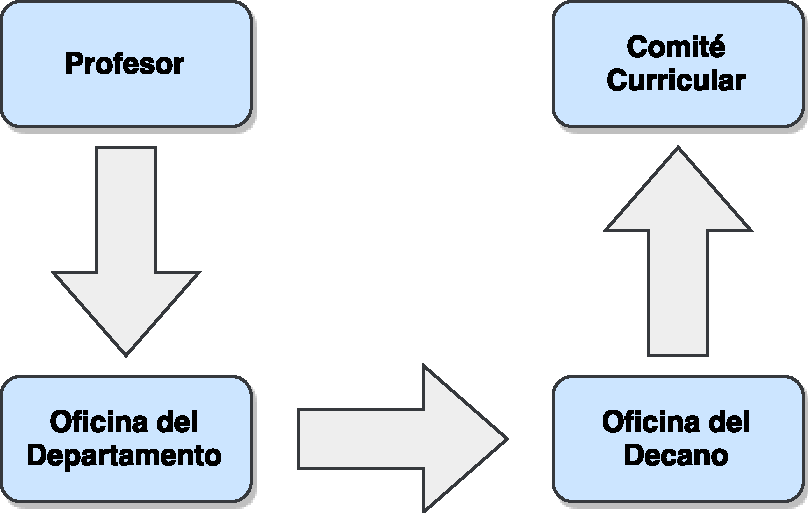
\includegraphics[scale=0.5]{Capitulos/MarcoTeorico/Imagenes/flujo_autoridades}
\caption{Flujo de creación y revisión de propuestas.}
  \label{flujo_autoridades}
\end{figure}

Hoy día el estado de California cuenta con un patrón de definición de cursos y programas donde la misma sirve como guía para el desarrollo de propuestas para material académico de las universidades. Dicho estándar además contiene una taxonomía de programas e indica cuál es el flujo para la revisión de las propuestas, donde todo es establecido en el PCAH\footnote{de sus siglas en inglés, Program and Course Approval Handbook, que significa en español manual de aprobación de cursos y programas.}.

El flujo inicia con el profesor o encargado del curso o programa, una vez completado pasa por la mesa de recepción donde se verifica que cumpla con el estándar estatal para luego pasar por la oficina departamental y la oficina del decano para su revisión de contenido. Una vez revisado y con el visto bueno de ambas oficinas pasa por una última revisión por parte de la oficina curricular para ser registrada en los sistemas de gestión curricular (figura \ref{course_creation_flow}).

Es un proceso que se hace con formularios en papel donde el profesor o encargado del curso o programa tiene que completar los campos requeridos para que el estado de California cuente al curso como válido. Dicho proceso tiene varias deficiencias como las que estaremos citando a continuación:
\begin{itemize}
	\item La creación o revisión puede tomar meses debido a los formularios que son completados a mano y requieren de revisión de varias oficinas.
	\item Es un flujo de una sola dirección, eso quiere decir que si es que una de las oficinas rechaza el formulario debe volver a iniciar el flujo.
	\item Se puede producir cuellos de botella en los diferentes puntos de revisión.
\end{itemize}

Una vez ya registrado en los sistemas de gestión curricular es accesible de manera pública para el uso de las universidades del estado de California. De esta manera, si una institución académica posee un sistema de gestión de evaluaciones y quiere incluir los cursos o programas válidos para el estado tiene ingresar los nuevos datos del sistema de gestión curricular uno a uno como se puede apreciar en la figura \ref{after_creation}.

\begin{figure}
\centering
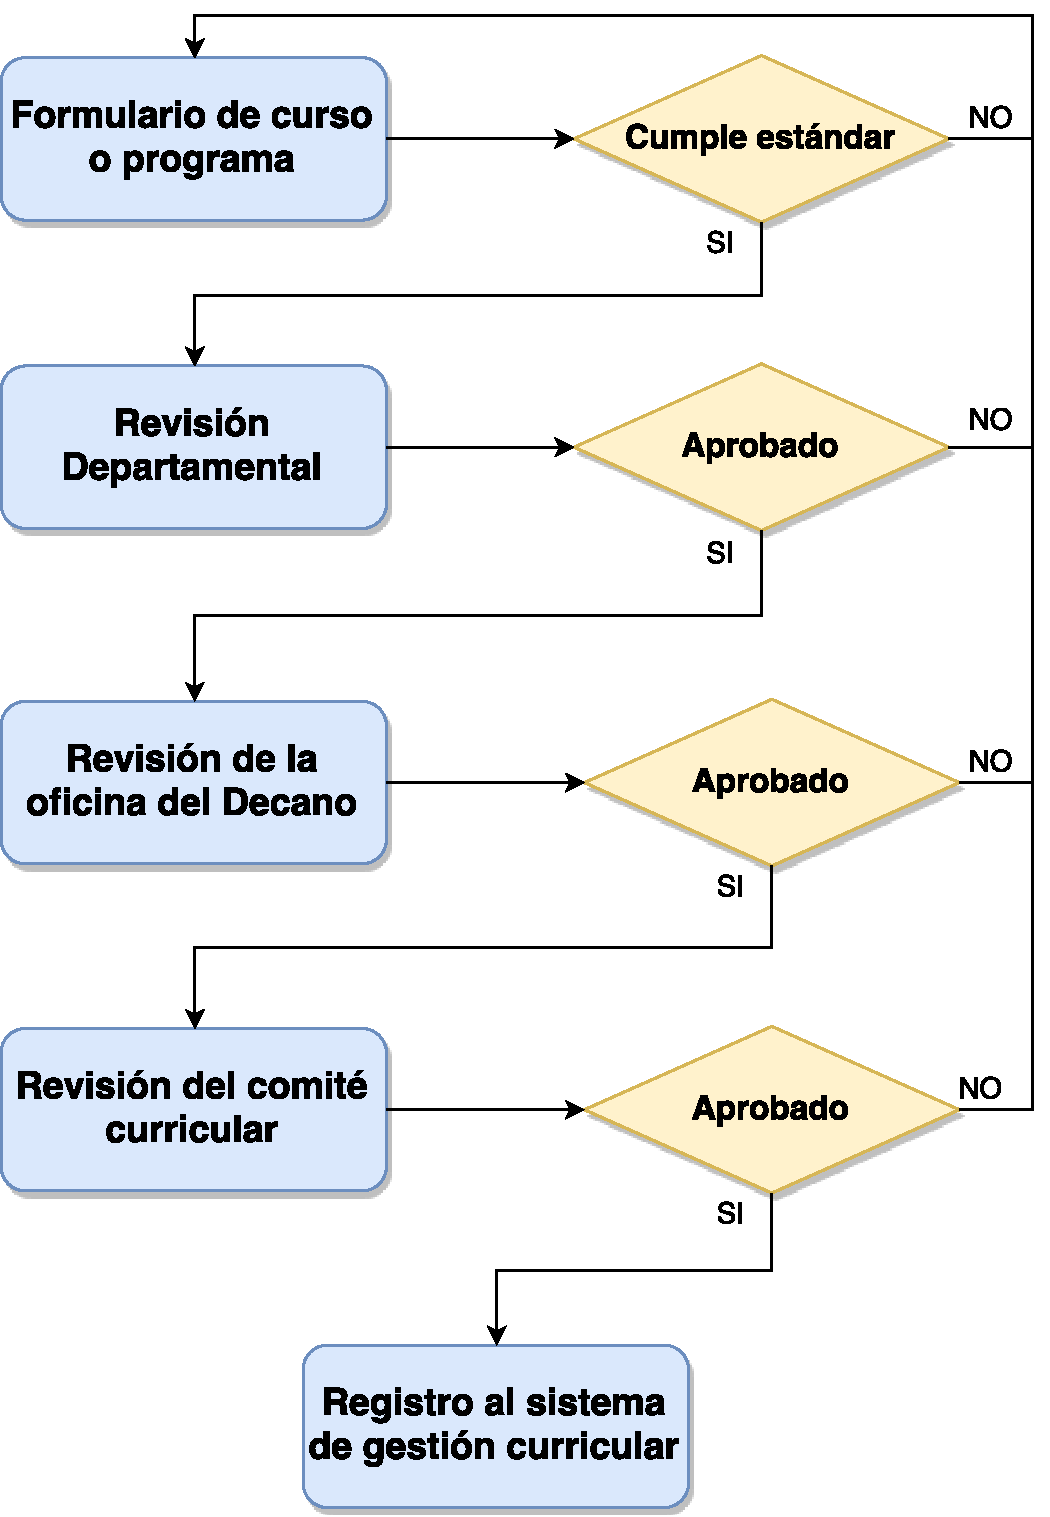
\includegraphics[scale=0.5]{Capitulos/MarcoTeorico/Imagenes/course_creation_flow}
\caption{Flujo actual de diseño de cursos, programas y competencias.}
  \label{course_creation_flow}
\end{figure}

\begin{figure}
\centering
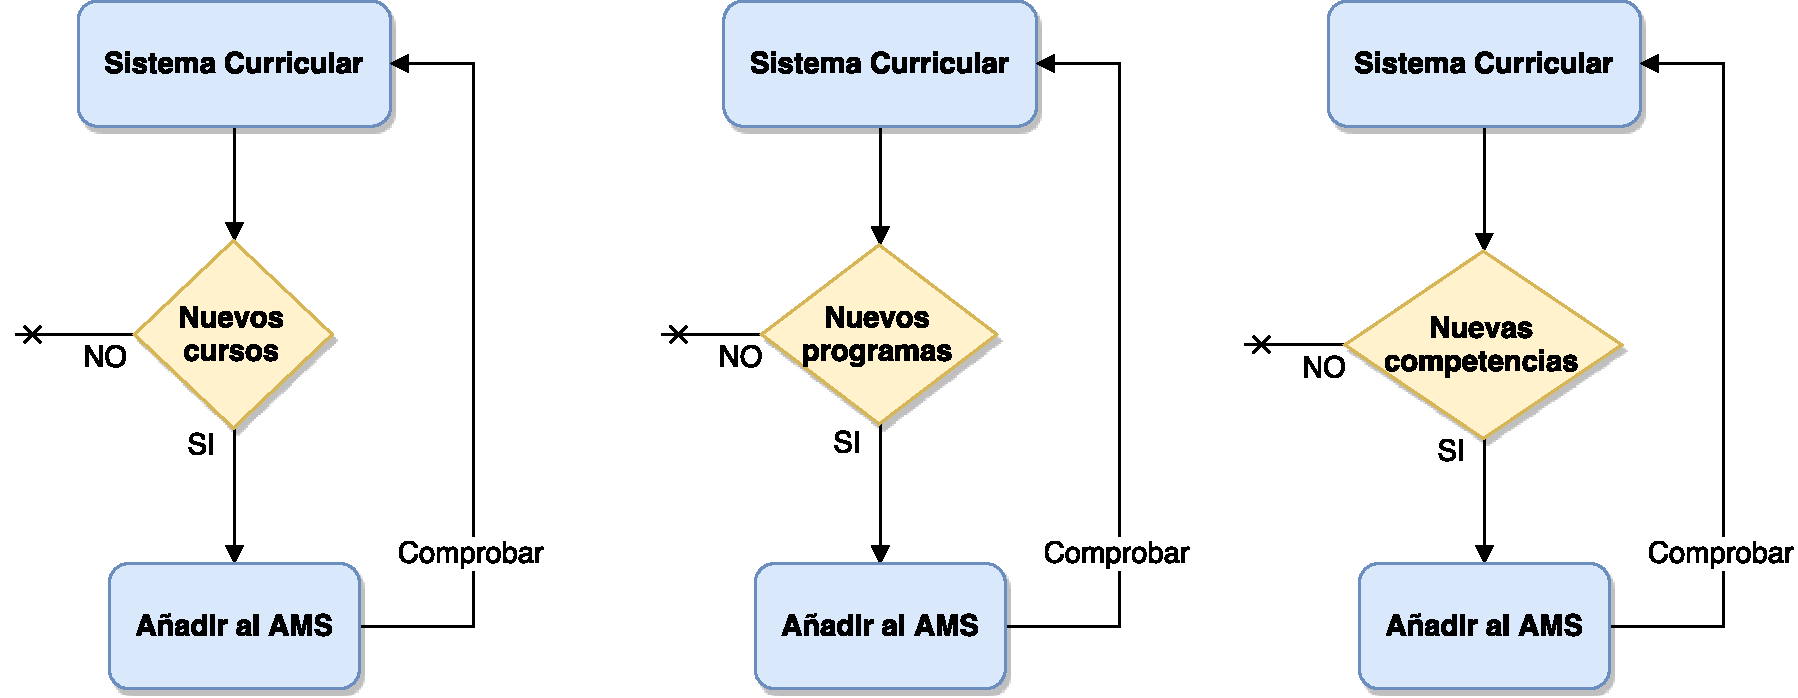
\includegraphics[width=125mm,scale=1]{Capitulos/MarcoTeorico/Imagenes/after_creation}
\caption{Esquema de tipos de computación en la nube.}
  \label{after_creation}
\end{figure}
\section{Sistemas de gestión curricular}
Un CMS \footnote{de sus siglas en inglés, Curriculum Management System, que significa sistema de gestión curricular} es un aplicación automatizada que apoya todo el proceso curricular, desde la planificación hasta la implementación y evaluación. Posee una interfaz única y cohesiva en línea que permite proponer, crear, evaluar, revisar, aprobar y aplicar cursos, programas y competencias\citep{harden2001amee}.

Curriculum es una mezcla sofisticada de estrategias educativas, contenido del curso, resultados de aprendizaje, experiencias educativas y evaluación. Esta visión amplia de un CMS se deriva del ambiente actual de educación elemental y secundaria que es impulsado por los estándares de contenido de cursos obligatorios federales y estatales, y la necesidad de auditorías continuas de currículo\citep{west2000technology}.

En los enfoques actuales del desarrollo de Curriculum por lo general gira en torno a los comités curriculares. Un comité curricular departamental comienza el proceso de desarrollo curricular considerando como entrada cualquiera de los aspectos mostrados en la figura \ref{diseno_curricular}.

\begin{figure}[H]
\centering
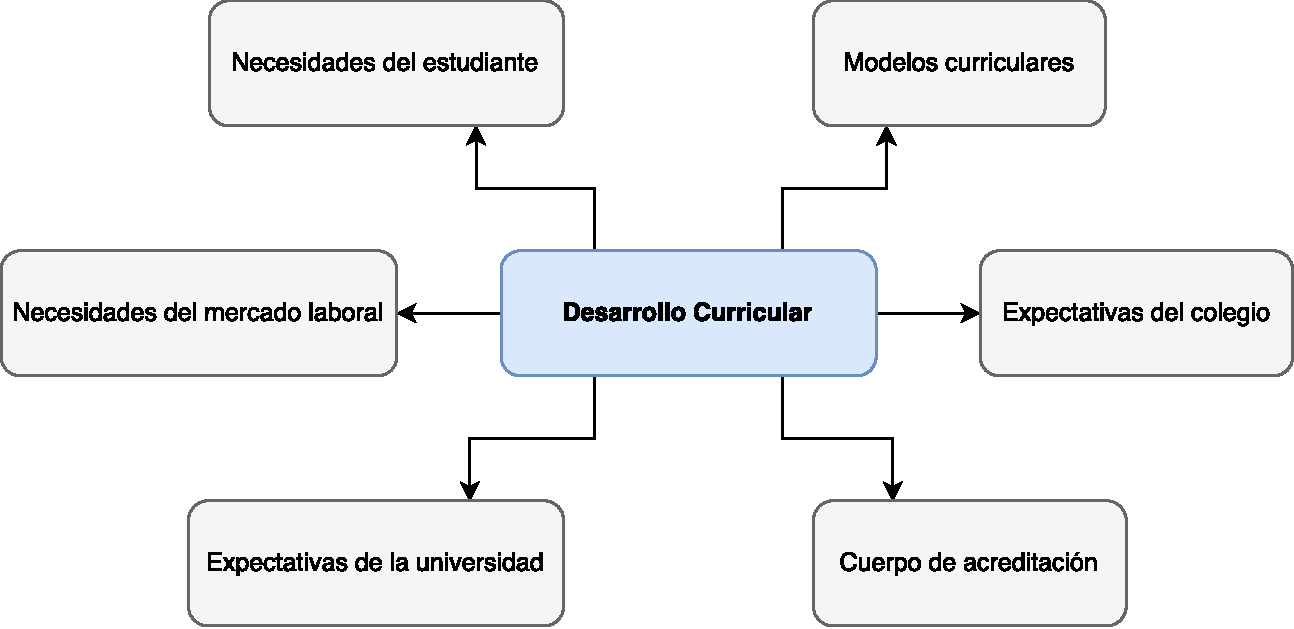
\includegraphics[width=125mm,scale=1]{Figuras/diseno_curricular}
\caption{Esquema de diseño curricular y sus variables determinantes.}
  \label{diseno_curricular}
\end{figure}


Dichos aspectos, sin embargo, sólo se consideran en un alto nivel de abstracción basado en la comprensión tácita de los miembros del comité sobre la disciplina.
\section{Aplicaciones web}
La necesidad de ejecución de operaciones complejas de manera remota y portable, tales como el uso de software sin depender de la potencia del hardware del usuario, la disponibilidad de uso en múltiples plataformas, y muchas otras, han guiado al desarrollo y evolución de las aplicaciones web. En las ciencias de la computación, una aplicación web es un software con arquitectura cliente-servidor donde el cliente (o interfaz de usuario) corre en un navegador web\citep{net_app_architecture}.

Los usuarios acceden a la aplicación utilizando un navegador web y no es necesario descargarse ningún tipo de software adicional, ya que la aplicación se ejecuta en el servidor. Para esclarecer el panorama, la lógica de la aplicación web se ejecuta remotamente, y el navegador web sólo se limita a la representación de los datos.

La evolución de las aplicaciones web ha crecido tan vertiginosamente que además de ofrecer una multitud de servicios, mejoran la UX a través de interfaces gráficas impactantes e intuitivas para los usuarios\citep{myers_past_2009}.
\section{Cloud computing}
Casi toda solución de infraestructura remota es llamada hoy día con el termino de computación en la nube o simplemente la nube.

La computación en la nube es una metáfora para abastecimiento y consumición de recursos de infraestructura. El nivel de abstracción ofrecida por la nube puede variar de hardware virtual a complejos sistemas distribuidos, debido a que los recursos están disponibles a demanda en enormes cantidades y pagados por uso\citep{wittig_amazon_2016}.

La infraestructura remota o nube puede ser manejada por una organización abierta para uso público, o puede ser privada, donde una nube que virtualiza y comparte la infraestructura con una sola organización o híbrida como son mostrados en la figura \ref{cloud_types}.

\begin{figure}[H]
\centering
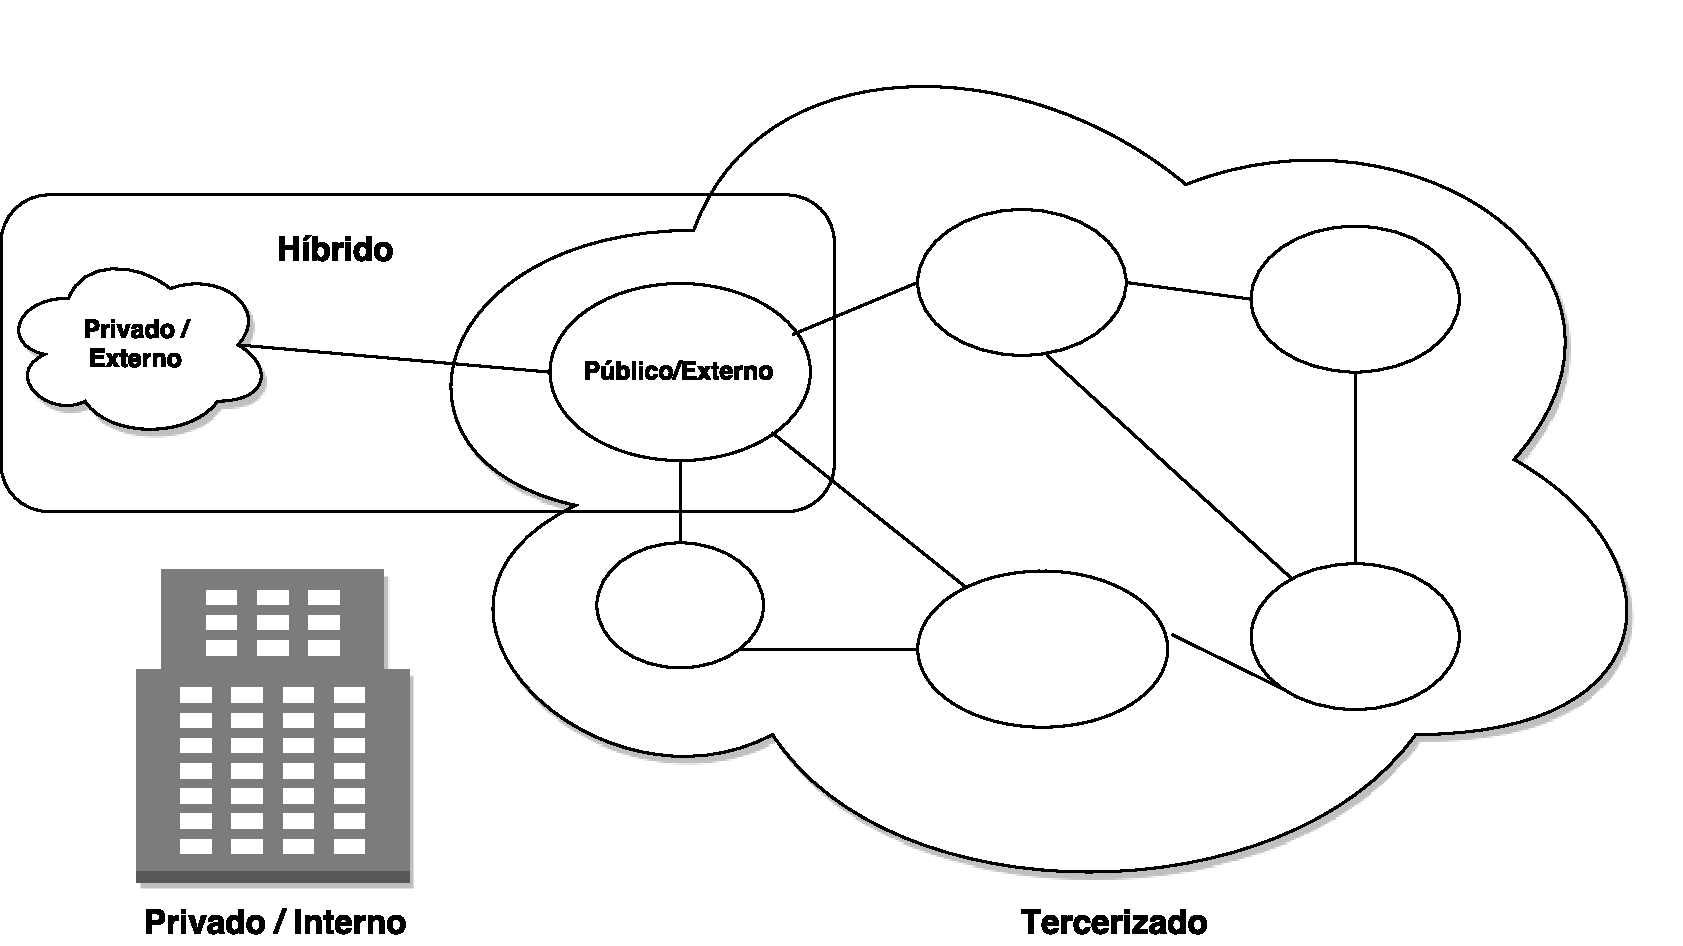
\includegraphics[width=125mm,scale=1]{Figuras/cloud_computing_types}
\caption{Esquema de tipos de computación en la nube.}
  \label{cloud_types}
\end{figure}
\section{Software as a Service}
SaaS\footnote{de sus siglas en inglés, Software as a Service, que significa en español software como servicio.}, es un paradigma de entrega de software donde la misma se encuentra alojada por lo general en la nube y se entrega como servicio a través de Internet a un gran número de usuarios a través de un modelo de suscripción. Se trata de un modelo de entrega de negocio en el que tanto la aplicación y el alojamiento son gestionados y compartidos con varias empresas, que alquilan y utilizan los servicios de aplicaciones de forma centralizada\citep{gupta_software_2014}.

El software como servicio es equivalente a servicios de proveedores externos que manejan todo mantenimiento, personalización, actualización y cobro para los servicios que su cliente utiliza de manera mensual o anual. El proveedor se encarga de ofrecer el software basado en un conjunto de códigos y datos definidos junto a las diferentes configuraciones para los diferentes clientes. Los suscriptores al servicio acceden a la aplicación con la sensación de que son los únicos usuarios de la aplicación. Sin embargo, los cambios de configuraciones como cambios de datos, flujo de trabajo, interfaz y el flujo de negocio son realizados de manera masiva y transparente para ellos\citep{kumar_cloud_2012}\citep{kang_web_2012}.

También existen otras opciones como PaaS\footnote{de sus siglas en inglés, Platform as a Service, que significa en español plataforma como servicio.} e IaaS\footnote{de sus siglas en inglés, Infraestructure as a Service, que significa en español infraestructura como servicio.}.

\subsection{Características}
Entre las características relevantes de las aplicaciones SaaS, y las que las remarcan como aplicaciones bien construidas, son desarrolladas a la medida, escalables y soportan multitenancy\footnote{En español se conoce como multiples clientes inquilinos, se refiere cuando varios clientes pueden utilizar la misma instancia.}. No todas las aplicaciones SaaS comparten todas las características, pero las más comunes son las siguientes: 

A nivel de la configurabilidad, las aplicaciones con esta característica poseen el mismo código base y provee a instancias con múltiples opciones de configuración tal que cada cliente pueda tener sus propias configuraciones de software únicas y pueda tener la sensación de que es el único usuario en utilizar la aplicación. Esta es la clave del éxito para las aplicaciones SaaS\citep{jadeja2012cloud}. Por ejemplo, cada cliente puede tener configurado su sitio para que muestren fondos de pantallas o logos en las páginas de inicio de sesión o páginas principales que ellos especifican. Esta característica también puede ser llamada personalización de la aplicación.

Desde la óptica del concepto de Multitenancy, una sola instancia de la aplicación corriendo puede servir a una cantidad de clientes. Los diferentes modelos de datos que están disponibles para soportar SaaS son las bases de datos aisladas, arquitectura de bases de datos aisladas compartidas y la construcción de datos\citep{lee2012web}. Utilizando la arquitectura multitenant los proveedores de aplicaciones SaaS pueden innovar de forma sencilla y ahorrar tiempo valioso gastado en mantener varias versiones de código deprecado y/o desactualizado\citep{kang2011design}.

Por otro lado se tiene el criterio de escabilidad, el cual es una de las características más complicadas de agregar a una aplicación SaaS debido a su elevado costo. La escalabilidad es soportada por la virtualización, pero teniendo en cuenta el costo y el problema de complejidad muchas veces el desarrollador de la aplicación no se complica con esta característica\citep{li2012cooperative}.

Además, aparte de las características mencionadas anteriormente, algunos beneficios que poseen las aplicaciones con arquitectura SaaS son las siguientes: \citep{li2012cooperative}\citep{ma2007business}\citep{chou2008software} 
\begin{itemize}
	\item Las aplicaciones SaaS pueden ser utilizadas por los usuarios por medio de sus navegadores Web. Esto ahorra en costos operacionales para el usuario junto con los requerimientos de hardware mínimo, por lo tanto, reduce el costo que el usuario necesita gastar en hardware.  Además de los costos de mantenimiento, costos de licencias del software también son minimizados.
	\item Mejor utilización de recursos, debido a que los recursos requeridos por las aplicaciones con arquitectura SaaS son mínimos.
	\item El avance de la tecnología Web permite que los proveedores de SaaS se ubiquen en el extranjero y también ofrezcan servicios de alta calidad. De esta manera, permite a los usuarios de la aplicación ahorrar en infraestructura.
	\item Usualmente, las soluciones SaaS residen en entornos en la nube donde son escalables y poseen integración con otras ventajas SaaS. En comparación al modelo tradicional, los usuarios no tienen que comprar otro servidor o software.
\end{itemize}
\section{Metodología Ágil de desarrollo de software}
La metodología Ágil envuelve un enfoque para la toma de decisiones en los proyectos de software, que se refiere a métodos de ingeniería del software basados en el desarrollo iterativo e incremental, donde los requisitos y soluciones evolucionan con el tiempo según la necesidad del proyecto. Los métodos tradicionales, como Waterfall, pretenden ser capaces de modelar completamente el dominio del problema de entrada y luego esperar que se produzcan pequeños cambios (o inclusive ninguno)\citep{davis_agile_2015}. Los métodos ágiles asumen que el cambio es inevitable, por lo que abordan el desarrollo de software de tal manera a facilitar la adaptación de los nuevos requisitos mientras vayan surgiendo.

Las metodologías ágiles, en comparación a otras metodologías de desarrollo, ofrecen un modelo de diseño flexible que fomenta al desarrollo evolutivo. Los desarrolladores trabajan en pequeños módulos cada vez y la retroalimentación proveída por el cliente ocurre simultáneamente en el desarrollo. Además, la metodología puede ser bastante útil en situaciones donde los objetivos finales del proyecto no están claramente definidos donde los requisitos del cliente se clarificarán gradualmente a medida que el proyecto avance.

El uso de la metodología ágil como método de entregas de las características del módulo entra como requisito no funcional.

\subsection{Historias de usuario}
Las historias de usuario conforman la parte central de muchas metodologías de desarrollo ágil, tales como XP\footnote{de sus siglas en inglés, eXtreme Programming, que significa en español programación extrema}, Scrum, entre otras. Estas definen lo que se debe construir en el proyecto de software, tienen una prioridad asociada definida por el cliente de manera a indicar cuales son las más importantes para el resultado final. Son divididas en tareas y su tiempo es estimado por los desarrolladores.

Por lo general, se espera que una estimación de tiempo de cada historia de usuario se sitúe entre horas y el tiempo máximo de iteración. Estimaciones superiores a este tiempo máximo son indicativas de que la historia es muy compleja y debe ser dividida en varias historias.

Una historia de usuario es una representación de un requisito escrito en una o dos frases utilizando el lenguaje común del usuario\citep{davis_agile_2015}. Ellas son utilizadas para la especificación de requisitos acompañadas de las discusiones con aquellos y las pruebas de validación.

Cada historia de usuario debe ser limitada. La metodología estipula que las mismas deben ser escritas por los clientes. Son una forma rápida de administrar los requisitos sin tener que elaborar gran cantidad de documentos formales y sin requerir de mucho tiempo para administrarlos.

Las historias de usuario deben ser:
\begin{itemize}
    \item \textbf{Independientes:} de ser necesario, combinar las historias dependientes o buscar otra forma de dividir las historias de manera que resulten independientes.
    \item \textbf{Negociables:} la historia en sí misma no es lo suficientemente explicita para considerarse un contrato, la discusión con los usuarios debe permitir esclarecerse y éste debe dejarse explicito bajo la forma de pruebas de validación.
    \item \textbf{Valoradas:} Los intereses de los clientes y de los usuarios no siempre coinciden, pero en todo caso, cada historia debe ser más importante para los clientes que para el desarrollador.
    \item \textbf{Pequeñas:} las historias grandes son difíciles de estimar e imponen restricciones sobre la planificación de un desarrollo iterativo. Generalmente se recomienda la consolidación de historias muy cortas en una sola historia.
    \item \textbf{Estimables:} las historias completas en requerimientos de parte del equipo de desarrollo y de parte del cliente son estimables. Y por lo tanto, el equipo debe estar cómodo de puntuar las historias de usuario.
    \item \textbf{Verificables:} las historias de usuario cubren requerimientos funcionales, por lo generalmente son verificables. Cuando sea posible, la verificación debe automatizarse, de manera que pueda ser verificada en cada entrega del proyecto.
\end{itemize}

Las iniciales de estas características, con sus nombres en inglés, forman la palabra INVEST, que significa “inversión”. Es porque toda historia de usuario, si se construye bien, es una inversión.

Al momento de implementar las historias, los desarrolladores deben tener la posibilidad de discutirlas con los clientes. El estilo sucinto de las historias podría dificultar su interpretación, podría requerir conocimientos de base sobre el modelo, o podría haber cambiado desde que fue escrita.

Cada historia de usuario debe tener en algún momento pruebas de validación asociadas, lo que permitirá al desarrollador, y más tarde al cliente, verificar si la historia ha sido completada. Como no se dispone de una formulación de requisitos precisa, la ausencia de pruebas de validación concertadas abre la posibilidad de discusiones largas y no constructivas al momento de la entrega del producto.

\subsection{Épicas}
Una épica es esencialmente una historia de usuario de un tamaño mucho mayor, siempre superior al tiempo de iteración máximo, y tiene como propósito el de asociar historias de usuario individuales relacionadas con un propósito de más alto nivel que cumplir. La misma es, por lo general, muy grande para que un equipo del proyecto pueda trabajar directamente sin partir en diversas historias de usuario\citep{cobb2015project}.

El uso de las épicas en proyectos de gran tamaño ayuda a organizar tareas complejas en un tipo de estructura para que la interrelación de historias de usuario esté bien entendida. Por lo tanto, el diseño de épicas en el proceso de desarrollo es fundamental antes de comenzar cualquier proyecto.
\section{Interacción humano-computador}
En HCI definen la funcionalidad y la usabilidad de los sistemas que se desarrollan, donde la funcionalidad de un sistema es definida por un conjunto de acciones o servicios que son proveídas a los usuarios, sin embargo, el valor de la funcionalidad es verificada cuando es eficientemente utilizada por el usuario \citep{shneiderman_designing_2010}. La usabilidad de un sistema con cierta funcionalidad es el rango y grado por el cual el mismo puede ser utilizada de manera eficiente y adecuada para cumplir ciertas metas para ciertos usuarios. La eficiencia de un sistema es alcanzada cuando se cumple un balance entre la usabilidad y la funcionalidad \citep{nielsen_usability_2010}.

HCI es un diseño que debe producir un ajuste entre el usuario, la máquina y los servicios requeridos con el fin de lograr un balance óptimo entre la calidad y la eficiencia de los servicios.

La definición de la estrategia de UI\footnote{de sus siglas en inglés, User Interface, que significa en español experiencia de usuario.} es importante para una mejor usabilidad del sistema, donde este proceso debería comenzar antes que el diseño y desarrollo de las aplicaciones. Es la visión de una solución que necesite ser verificado con potenciales usuarios que prueben que necesite el mercado \citep{levy_ux_2015}.

% ESTADO DEL ARTE
\chapter{Estado del arte} % Main chapter title
En este capítulo realizamos un relevamiento y análisis de herramientas de informática educativa que intentan resolver problemas relacionados de forma cercana a los problemas planteados en este trabajo de tesis.

\label{capitulo3} % Change X to a consecutive number; for referencing this chapter elsewhere, use \ref{capitulo3}
\section{CurricUNET}
CurricUNET es una aplicación web diseñada para automatizar la emisión y aprobación del plan de estudios emitido por profesores y/o encargados de universidades norteamericanas; que incluyen programas, cursos y competencias.

En la misma se desarrollan propuestas de cursos y programas de estudio mediante formularios de la aplicación, con el objetivo de reemplazar solicitudes en papel que universidades utilizaban para emitir propuestas. Además, ofrece almacenamiento e información de plan de estudios históricos, activos y propuestos.

Todas las entradas, revisiones y reportes son accedidas por la web desde los navegadores. Posee un sistema de notificaciones integrado que permite al usuario un mejor seguimiento del progreso de las propuestas y cursos en revisión. Además, dispone de un control de versionamiento de cursos, planes de estudio y competencias.

Los usuarios del sistema pueden acceder a los reportes e historial de versiones de sus cursos y planes de estudio por lo que ayuda a una mejora continua del programa universitario.
\section{Courseleaf}
El módulo de Curriculum de CourseLeaf es una solución de gestión basada en la web, mejorando los procesos de profesores y del comité de Curriculum de al menos 70 instituciones\citep{courseleaf_webpage}.

Cuando el módulo de Curriculum de CourseLeaf se combina con su módulo de catálogo, colegios y universidades son capaces de gestionar y realizar un seguimiento de la información del programa, desde la propuesta hasta publicar en una aplicación integrada con facilidad.

El software proporciona la generación de flujo de trabajo automático, notificaciones automáticas. Además, identifica todos los cursos, programas y departamentos que se ven afectados por los cambios propuestos en el inicio del proceso de propuesta y puede ayudar en la actualización con los cambios completados. El módulo de Curriculum de CourseLeaf se puede implementar con o sin su catálogo de Cursos.

El módulo de Curriculum dispone de cuatro componentes:
\begin{itemize}
	\item Un listado de cursos donde los usuarios pueden encontrar información sobre el curso. También pueden iniciar, editar y presentar propuestas de cursos.
	\item Una interfaz de los usuarios autorizados a opinar, anotar, rechazar, y aprobar las propuestas.
	\item Un formulario de curso, un formulario dinámico con campos inteligentes y el formato de respuesta que optimiza la experiencia del usuario.
	\item Un formulario de los programas, utilizando la misma funcionalidad que los formularios de curso para proponer y mantener la información y los requerimientos para los programas y grados.
\end{itemize}
\section{DECA: Curriculum Navigator}
DECA ofrece, mediante su módulo de Curriculum Navigator, una solución de desarrollo y administración de Curriculum.

Frecuentemente, descrito como complejo e ineficaz, los métodos tradicionales basados en papel de gestión de programas de estudio proporcionan una visibilidad limitada, lo que resulta en una visión restringida de las etapas implicadas en la creación, modificación y aprobación de planes de estudio. Además, busca eliminar esta complejidad al acelerar el desarrollo curricular y el proceso de aprobación.

Cuando se utiliza como módulo integrado de su Catálogo, denominado como Catalog Navigator, proporciona una solución que les permite iniciar el camino de aprobación de alguna carrera de grado. Asesores y administradores, por otra parte, utilizan tanto Curriculum Navigator y Catalog Navigator para desarrollar y proporcionar datos públicamente del plan de estudios para sus estudiantes actuales y futuros.

Curriculum Navigator ofrece:
\begin{itemize}
	\item El acceso a un repositorio de datos curricular.
	\item Editar, guardar y proponer planes de estudio o carreras de grado.
	\item Historial de cambios y de accesos de revisión.
	\item Seguimiento en tiempo real de propuestas abiertas.
\end{itemize}
\section{Comparación entre plataformas}
Una investigación para comprobar otros proyectos o productos con las mismas características propuestas, buscando innovación para el mercado es expuesta en la tabla \ref{relacion-sistemas}.

\begin{table}[H]
\centering
\resizebox{\columnwidth}{!}{%
	\begin{tabular}{lllccl}
		\toprule
		\multicolumn{3}{l}{Características}                                                & CurricUNET                       & CourseLeaf            & DECA         \\
		\midrule
		\multicolumn{3}{l}{Creación y versionamiento de competencias.}                     &                                  &                       &              \\
		\multicolumn{3}{l}{Creación y versionamiento de cursos.}                           & $\checkmark$                     & $\checkmark$          & $\checkmark$ \\
		\multicolumn{3}{l}{Creación y versionamiento de programas de estudio.}             & $\checkmark$                     & $\checkmark$          &              \\
		\multicolumn{3}{l}{Cumple los Estándares de códigos de California.} 			   & $\checkmark$                     &                       &              \\
		\multicolumn{3}{l}{Historial de versiones de competencias.}     			       & 			                      & 		              &  			 \\
		\multicolumn{3}{l}{Historial de versiones de cursos.}     			               & $\checkmark$                     & $\checkmark$          & $\checkmark$ \\
		\multicolumn{3}{l}{Historial de versiones de programas de estudio.}     		   & $\checkmark$                     &  			          & 			 \\
		\multicolumn{3}{l}{Reporte de Comparación entre versiones de cursos.}              & $\checkmark$                     &                       & $\checkmark$ \\
		\multicolumn{3}{l}{Soporta competencias de aprendizaje del estudiante.}            &                      			  &                       &              \\
		\multicolumn{3}{l}{Plantilla de flujo de trabajo customizable.}                    & $\checkmark$                     &                       &              \\
		\multicolumn{3}{l}{Permite asignar roles evaluadores en la aplicación.}            & $\checkmark$                     & $\checkmark$          &              \\
		\multicolumn{3}{l}{Permite asignar usuarios como colaboradores.}                   & $\checkmark$                     &                       &              \\
		\multicolumn{3}{l}{Sistema de alertas para colaboradores y evaluadores.}           & $\checkmark$                     & $\checkmark$          &              \\
		\multicolumn{3}{l}{Buzón de entrada para colaboradores y autoridades.} 			   & $\checkmark$                     &                       & $\checkmark$ \\
		\multicolumn{3}{l}{Soporte de correlatividades entre cursos.}                      & $\checkmark$ 					  &						  &              \\
		\multicolumn{3}{l}{Incluye un catálogo de cursos.}                   		   	   & $\checkmark$					  &	$\checkmark$		  & $\checkmark$ \\
		\multicolumn{3}{l}{Incluye un catálogo de programas de estudio.}                   & $\checkmark$					  &	            		  &              \\
		\multicolumn{3}{l}{Incluye un catálogo de competencias.}                   	       & 								  &						  & 			 \\
		\multicolumn{3}{l}{UX intuitiva y efectiva.}     			   					   &                                  & $\checkmark$          & $\checkmark$ \\
		\bottomrule
	\end{tabular}
}
\caption{Relación entre sistemas de gestión curricular.}
\label{relacion-sistemas}
\end{table}

Los puntos de la tabla \ref{relacion-sistemas} fueron elegidos a base de una encuesta a los clientes, donde se les preguntó cuáles son las necesidades que tiene una universidad a la hora de proceder al diseño de cursos y programas de estudio. Además, como funcionalidad adicional se les ofreció la capacidad de soportar las competencias de sus universidades, y como se obtuvo una respuesta positiva de su parte se decidió agregar como un punto más en la tabla, para corroborar luego con el análisis de las diferentes herramientas si no soportaban dichas funcionalidades. Fueron tres los CMS que existen que cumplen con las expectativas mínimas del mercado y son a las cuáles se les hizo el análisis.

De los CMS existentes, CurricUNET es el que más satisface las necesidades de las universidades, pero al no soportar competencias ni ser capaz de adaptarse a un AMS de las universidades comunitarias del estado de California impide la creación automatizada de entidades validadas en un solo proceso.
\section{Relevancia del módulo curricular}
La importancia del módulo reside en la posibilidad de automatizar formularios y procesos que requieren la participación de personas ajenas al flujo de trabajo para iniciar y validar propuestas de creación o revisión de cursos y programas. Sin embargo, hay alternativas que buscan solucionar la misma problemática pero se existe alternativa que pueda soportar el uso de competencias ni que pueda comunicarse con un sistema de gestión de evaluación basadas en competencias.

Como se hablo en la sección \ref{procesoCurricular} de proceso curricular; una vez finalizado el proceso de diseño y revisión curricular de parte de las oficina, se procede a publicar la nueva competencia, curso, o programa para que se puedan cada universidad tenga la información necesaria para ir cargando dicha información en sus correspondientes sistemas, en el caso de las universidades comunitarias del estado de California se utilizan los AMS para gestionar y evaluar las competencias de sus estudiantes. El proceso de registro de las nuevas entidades en los AMS es individual; eso quiere decir que un encargado del AMS debe encargarse de cargar uno por uno las nuevas entidades aprobadas y publicadas por el comité curricular.

En la propuesta de solución (capítulo \ref{capitulo5}) hablaremos de como el proyecto final busca solucionar la problemática y unir los procesos de los cuales hablamos en el párrafo anterior.

\section{Sumario}
Se han expuesto las investigaciones hechas por el equipo de expertos en didáctica en modo de encuestas a los usuarios finales de las necesidades y funcionalidades que buscan o utilizan en las alternativas de CMS que utilizan en sus universidades. 

Además, se realizaron análisis como investigación de campo de las herramientas que buscan resolver la misma problemática, en una tabla comparativa de las diferentes opciones con las necesidades de los usuarios finales expuestas anteriormente y la relevancia del proyecto.

% PROPUESTA DE SOLUCION
\chapter{Propuesta de solución} % Main chapter title
En este capítulo se presenta en detalle la arquitectura del sistema planteada como solución, con un correspondiente estudio para la determinación de las herramientas para cada paso. Se expone además el flujo de datos y se presenta un diseño del mismo, donde queda gráficamente los pasos a seguir. Se incluyen también las técnicas de validación y evaluación que se deben utilizar.

\label{capitulo4} % Change X to a consecutive number; for referencing this chapter elsewhere, use \ref{capitulo5}
En esta sección se proveerá una descripción detallada de los modelos obtenidos; en donde, se explicarán las funciones y los principales componentes de cada parte. Se inlcuyen figuras ilustrativas de los resultados de clustering obtenidos, así como la explicación de los parámetros considerados para cada algoritmo.

Una vez que los requerimientos iniciales han sido fijados y aclarados se busca la manera de automatizar los procesos, investigar tecnologías, y metodologías que ayuden al equipo de desarrollo para entregar funcionalidades de manera iterativa y evolutiva. Durante este proceso se diseñan modelos donde se propone el módulo a ser desarrollado (Figura \ref{curriculum_model}) y se busca unir procesos separados del diseño curricular (Figura \ref{course_creation_flow}) con el flujo de agregar las competencias, cursos, y programas al AMS (Figura \ref{after_creation}).

\begin{figure}[]
\centering
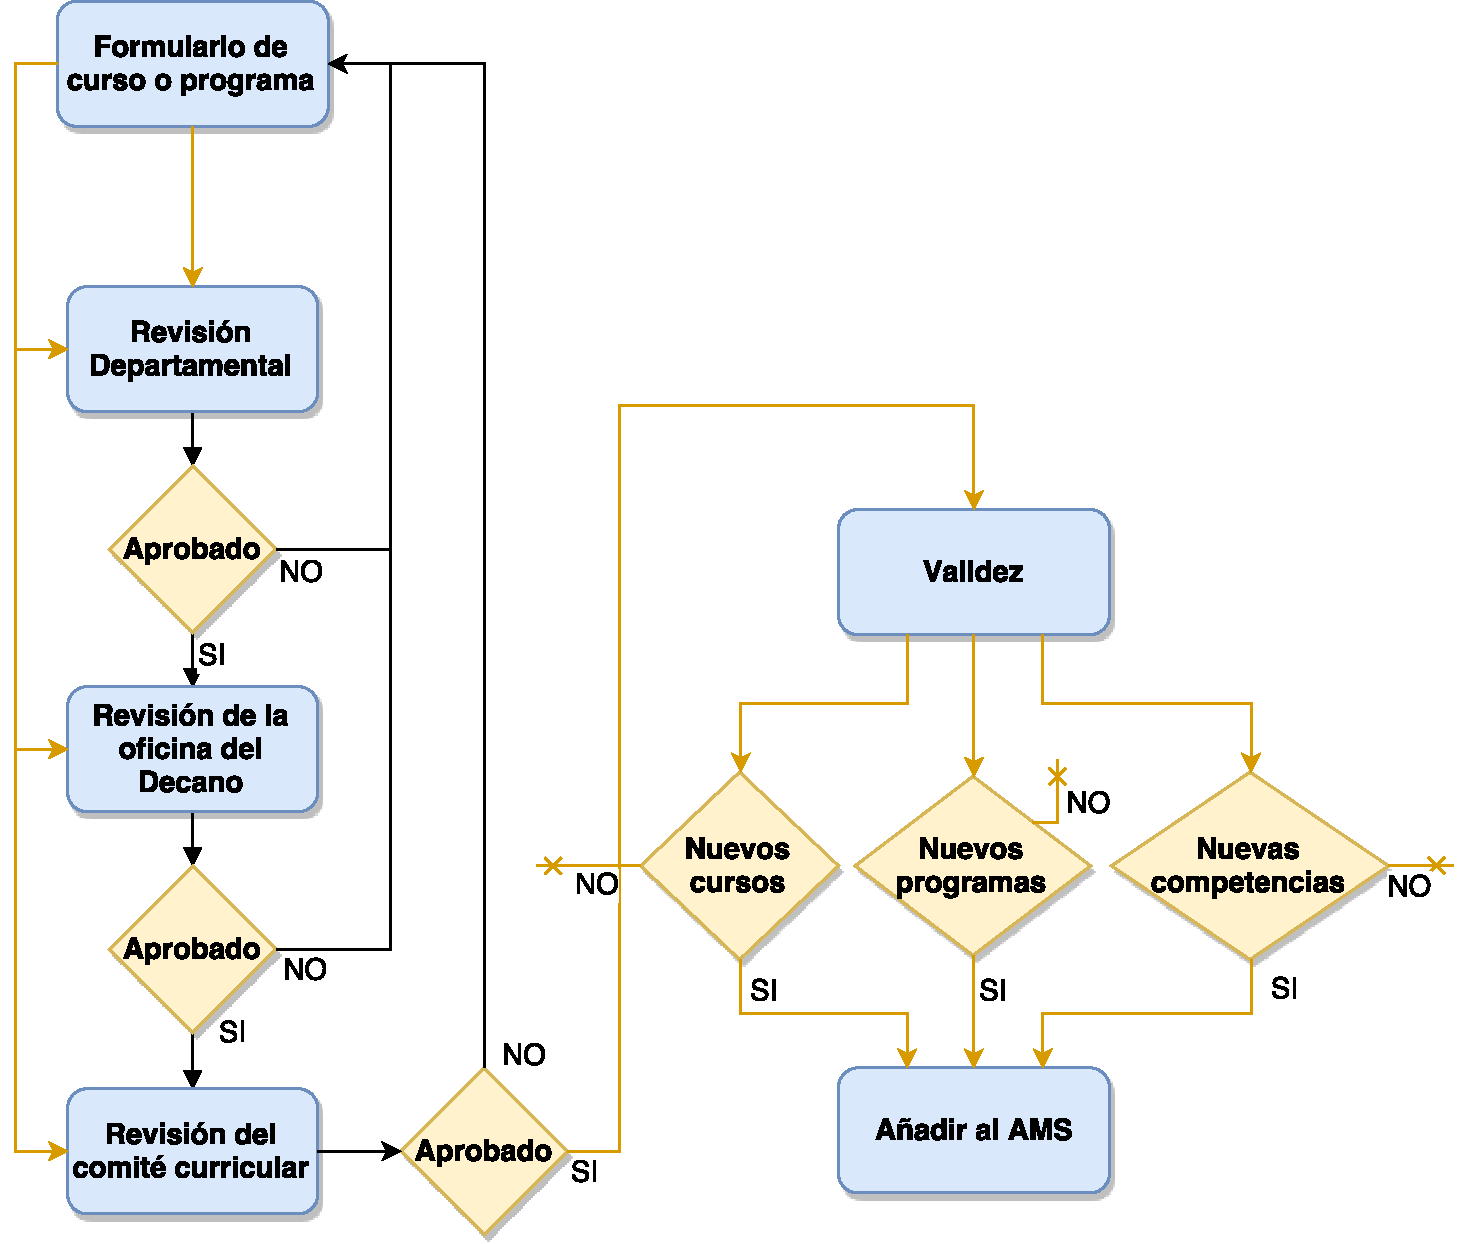
\includegraphics[scale=0.5]{Capitulos/PropuestadeSolucion/Imagenes/curriculum_model}
\caption{Modelo propuesto del módulo curricular adherido a un sistema de gestión de evaluaciones basadas en competencias.}
  \label{curriculum_model}
\end{figure}

Actualmente, cuando el encargado de curso o programa completa su formulario y lo entrega en la mesa de recepción, la misma se encarga de verificar que los datos completados sean válidos y cumpla con el estándar de creación de cursos y programas. 

El módulo propuesto se encargará de automatizar dicho proceso sacando la mesa de recepción como iniciador del flujo de validación mediante un formulario web. Además, se agrega un nuevo tipo de formulario para las competencias de las universidades comunitarias de California.

Luego, pasa por las oficinas del departamento, del decano, y del comité curricular para sus correspondientes revisiones. Si es que una de las oficinas rechaza el formulario debe volver al inicio con el encargado del mismo para volver a ser completado, y una vez terminado puede volver a pasar a la oficina que rechazó el formulario sin necesidad de volver a iniciar todo el proceso de corrección.

Y finalmente, una vez que el comité curricular acepta el formulario se procede a generar los nuevos cursos, programas, o competencias en el AMS. También, otro proceso a ser automatizado por el módulo ya que hoy día dicha creación se hace de manera manual, como se aprecia en la figura \ref{after_creation}.

Se agrega también la funcionalidad de mensajes generados y notificaciones a los integrantes del flujo para evitar de esta manera los cuellos de botella con las revisiones, donde se notifican los pendientes y alertan trabajos en deuda.

\section{Modelo de arquitectura de módulo}

\section{Requerimientos no funcionales} \label{reqnofuncional}
Se ha realizado una breve revisión de las tecnologías y abordajes brindadas como requerimientos funcionales. Sin embargo, al utilizar un abordaje ágil, la validación de las decisiones tecnológicas depende en última instancia de la validación del proceso de desarrollo realizada por expertos y usuarios.

Las decisiones de tecnologías para el módulo de gestión curricular fueron basadas en los conocimientos adquiridos de los miembros del equipo de desarrollo, con el fin de optimizar tiempos utilizados en curvas de aprendizaje. Sin embargo, se hicieron análisis previos a su uso para corroborar que dichas tecnologías cumplen con el propósito de desarrollo.

\subsection{Java}
La elección del lenguaje de programación, establecida por la organización, fue utilizada como lenguaje para la lógica del módulo curricular ya que facilita la integración con el código ya existente. El equipo de desarrollo posee conocimiento en este lenguaje de programación o en lenguajes orientados a objetos, por lo que se aprovechó el tiempo que pudo haber sido utilizado en curvas de aprendizaje del lenguaje para investigar buenas prácticas para el proyecto.

Java fue diseñado para alcanzar los desafíos del desarrollo de aplicaciones en el contexto de ambientes heterogéneos y distribuidos en red \citep{eckel_thinking_2006}. Lo más importante de solucionar entre estos desafíos era la entrega segura de aplicaciones que consumen lo mínimo de recursos del sistema, correr en cualquier plataforma de hardware y/o software, y que pueda ser extendido de manera dinámica \citep{sierra2005head}.

Operar en múltiples plataformas con redes heterogéneas invalida la arquitectura tradicional de distribución de binarios, \enquote{release}, actualización, parcheo, etc \citep{arnold2005java}.

Hoy día, Java es uno de los lenguajes de programación más utilizados a nivel mundial debido a su portabilidad y evolución con el paso del tiempo, como se observa en la Figura \ref{graph_java}. Además, al ser un lenguaje de programación multiplataforma cualquier proyecto se puede desarrollar en cualquier sistema operativo o plataforma para luego ser levantada en el servidor independiente a su plataforma. 

El lenguaje es reconocido por ser intuitivo a la hora de programar, altamente portátil y portable \citep{hunt2011java}. Por otra parte, la comunidad es uno de los fuertes de Java. Además, en la Web hay una gran cantidad de foros y librerías de la comunidad para resolver diferentes problemáticas de los desarrolladores.

\begin{figure}[]
\centering
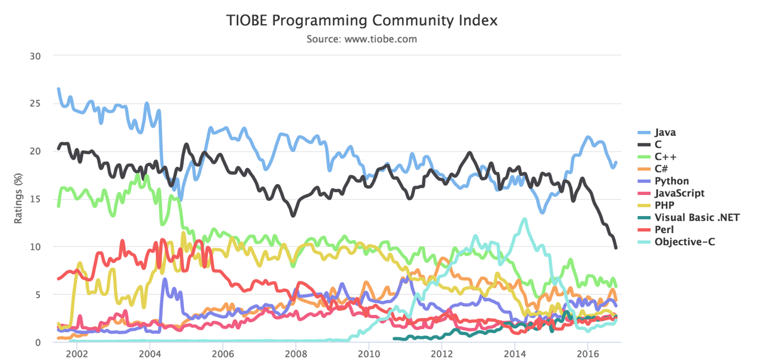
\includegraphics[width=125mm,scale=1]{Figuras/tecnologias/java}
\caption{Gráfico de uso de lenguajes de programación con respecto al tiempo \citep{tiobe_programming}.}
  \label{graph_java}
\end{figure}

El lenguaje Java proporciona un nivel de rendimiento adecuado para la plataforma donde se aloja el AMS.

Dicho uso del lenguaje fue validado durante el proceso de desarrollo al poder resolver los criterios de aceptación de las historias de usuario.

\subsection{MySQL}
Para ayudar a que el AMS sea adaptable y fácil de mantener, se extenderá la base de datos ya utilizada por el AMS. Por lo tanto, la elección de la base de datos del módulo queda a criterio de la organización y como requisito no funcional para el proyecto final. El sistema de base de datos que se utiliza para el sistema de evaluación de competencias es MySQL, por ser un sistema open source y con una de las comunidades más grandes entre las bases de datos existentes.

MySQL es el sistema de base de datos open source más popular disponible. Es particularmente eficaz para sitios web públicos que requieren base de datos rápidas y estables \citep{dyer2015learning}. Para añadir, acceder y procesar datos almacenados en una base de datos informática se necesita de un sistema de administración de Base de Datos como MySQL Server. 

Como las computadoras son muy buenas manejando grandes cantidades de datos, los sistemas de administración de base de datos juegan un rol principal en la computación como utilidades autónomas o como partes de otras aplicaciones.

Para representar los datos que se almacenan, utiliza el modelo lógico de datos relacional donde guarda sus datos en tablas separadas, antes que consolidar todos los datos en un solo lugar. La estructura de la base de datos está organizada en archivos físicos optimizados para mayor velocidad \citep{ronstrom2004mysql}. 

El modelo lógico con objetos tales como bases de datos, tablas, vistas, filas, y columnas, ofrecen un ambiente de programación flexible donde se establecen reglas que gobiernan las relaciones entre las de los distintos tipos de campos, tales como uno a uno, uno a muchos, únicos, requeridos, u opcionales y punteros entre diferentes tablas.

En las siguientes figuras \ref{graph_db_1} y \ref{graph_db_2} podemos observar que MySQL es un sistema de manejo de base de datos muy utilizado por la comunidad y va en aumento de popularidad hasta casi alcanzar a uno de los gigantes que es Oracle.

\begin{figure}[H]
\centering
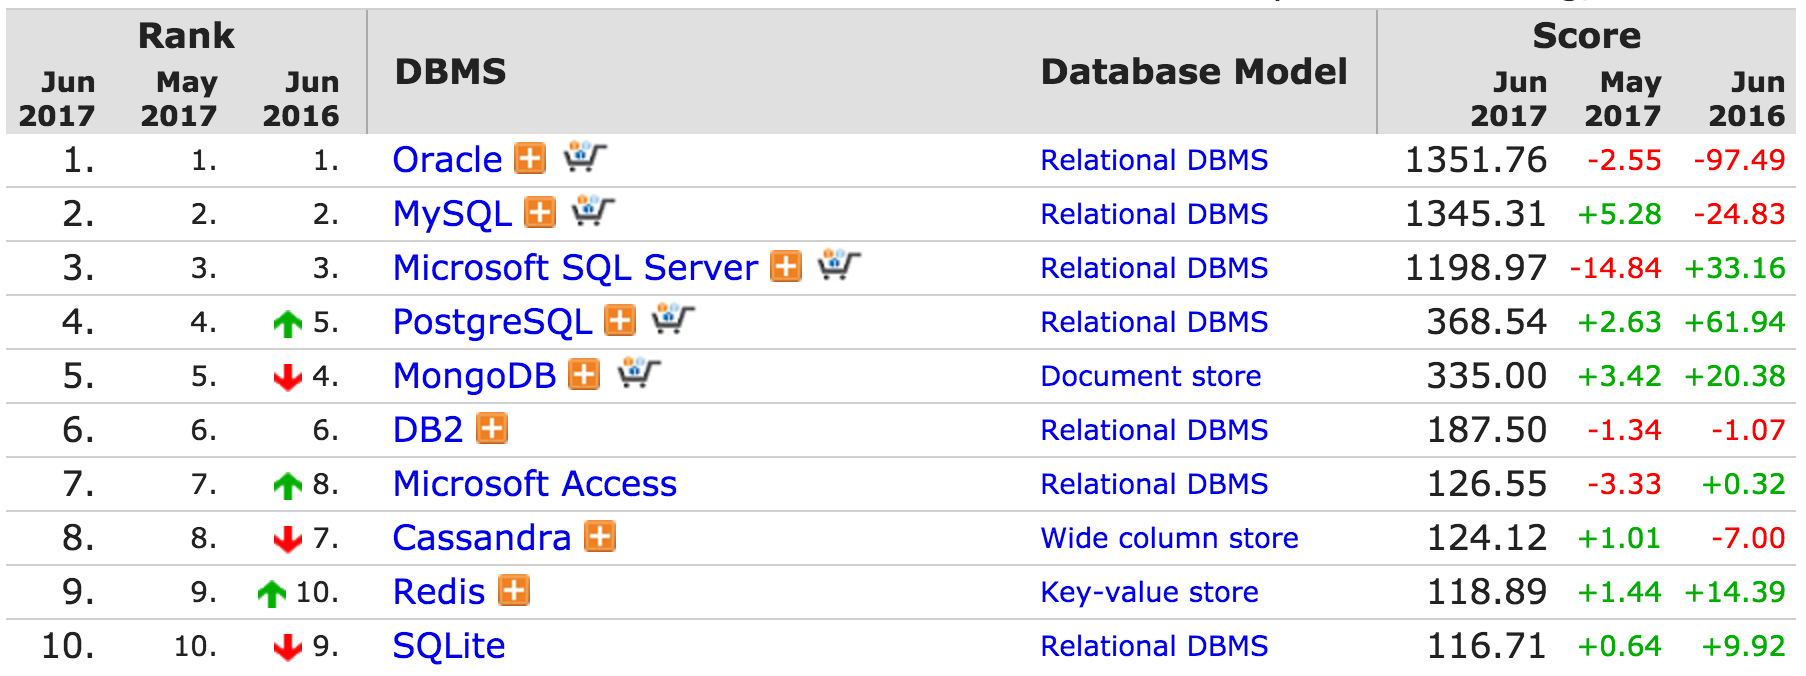
\includegraphics[width=125mm,scale=1]{Figuras/tecnologias/rank_db_1}
\caption{Gráfico que muestra el puntaje de uso de motores de base de datos \citep{db_engines_page}.}
  \label{graph_db_1}
\end{figure}

\begin{figure}[H]
\centering
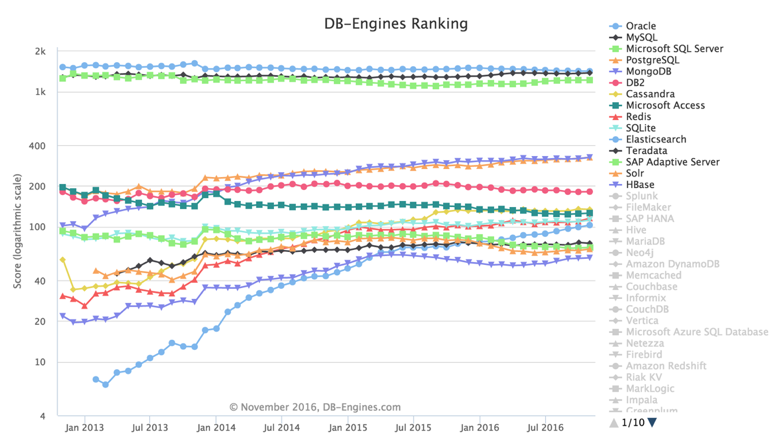
\includegraphics[width=125mm,scale=1]{Figuras/tecnologias/rank_db_2}
\caption{Gráfico de uso de motores de base de datos con respecto al tiempo \citep{db_engines_page}.}
  \label{graph_db_2}
\end{figure}

El motor de base de datos es otro requerimiento no funcional, ya que es otra tecnología utilizada para la aplicación base. Sin embargo, se hizo un breve análisis de vulnerabilidades para verificar que el uso de MySQL como base de datos relacional podría ser efectivo para el proyecto final, además, los desarrolladores están familiarizados con la misma.

\subsection{Amazon Web Services}
Amazon Web Services, o más conocida como AWS, es una plataforma de servicios web que ofrece soluciones de procesado, almacenamiento y redes en diferentes capas de abstracción. Se pueden usar estos servicios para hospedar sitios web, correr aplicaciones complejas y para minería de grandes cantidades de datos \citep{wittig2015amazon}. 

La interfaz web puede ser manejada por máquinas o por usuarios mediante de una interfaz de usuario gráfica. Los servicios más utilizados son EC2 en la cual ofrece servidores virtuales, y S3 que es utilizada para almacenamiento.

AWS es una nube pública, donde tiene las siguientes clasificaciones como nube:
\begin{itemize}
	\item \textbf{Infraestructura como Servicio:} más conocida como IaaS, ofrece recursos fundamentales como procesamiento, almacenamiento, y capacidades de servicios, utilizando servidores virtuales tales como Amazon EC2, Google Compute Engine y Microsoft Azure en las máquinas virtuales.
	\item \textbf{Plataforma como Servicio:} más conocida como PaaS, provee plataformas para desplegar aplicaciones customizadas a la nube, tales como AWS Elastic Beanstalk, Google App Engine, y Heroku.
	\item \textbf{Software como Servicio:} más conocida como SaaS, combina infraestructura y software corriendo en la nube, incluyendo aplicaciones de oficina como Amazon WorkSpaces, Google Apps for Work, y Microsoft Office 365.
\end{itemize}

En la figura \ref{graph_cloud} se puede mostrar como AWS lidera entre las alternativas del mercado para soluciones de computación en la nube. Luego, lo sigue Azure de Microsoft como siguiente alternativa más utilizada. AWS y Azure son líderes en opciones de cloud debido a su constante innovación en el mercado como se puede apreciar en la figura \ref{gartner_cloud}.

\begin{figure}[H]
\centering
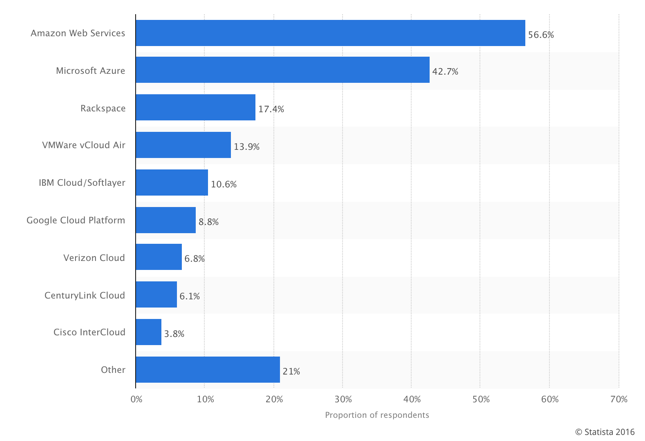
\includegraphics[width=125mm,scale=1]{Capitulos/PropuestadeSolucion/Imagenes/rank_cloud}
\caption{Ranking de compañías que brindan servicios de cloud computing \citep{statista_ranking}.}
  \label{graph_cloud}
\end{figure}

\begin{figure}[H]
\centering
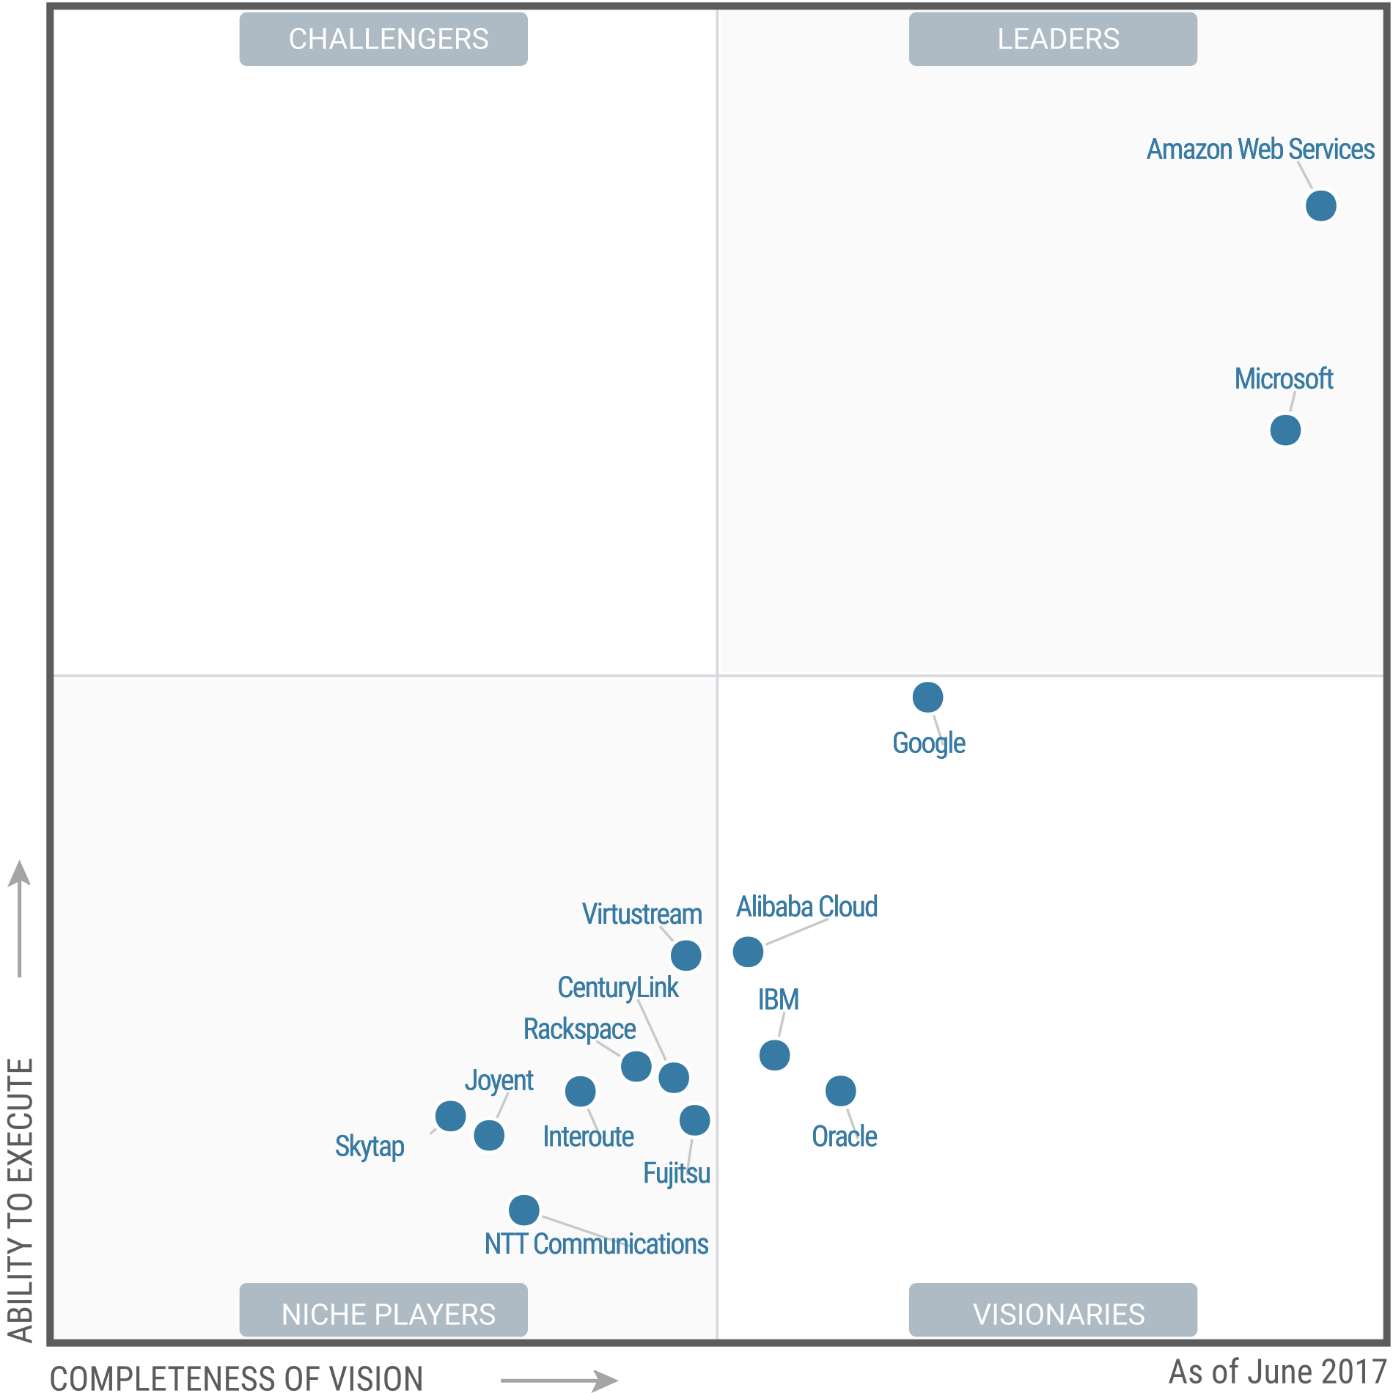
\includegraphics[scale=0.5]{Capitulos/PropuestadeSolucion/Imagenes/gartner_cloud}
\caption{Figura de Gartner que muestra las alternativas de cloud computing \citep{gartner_webpage}.}
  \label{gartner_cloud}
\end{figure}

El AMS se encuentra alojado en la plataforma de servicios AWS. Por lo tanto, se utilizaron los servidores ya en línea para correr el módulo curricular para la aplicación.

\subsection{Git}
Como un equipo de desarrollo requiere de un sistema de control de versiones eficiente, se utilizó Git por ser el líder en VCS \citep{loeliger2012version}. Para mejorar la integración del código que produce el equipo, la organización utiliza un repositorio en \enquote{GitHub}\footnote{Plataforma de desarrollo colaborativo de software para alojar proyectos utilizando el sistema de control de versiones Git.}. Además, el uso de un sistema de versionamiento permite minimizar y optimizar el tiempo de unión de módulos que van agregando o actualizando los miembros del equipo de desarrollo.

El control de versiones es un sistema que registra los cambios realizados sobre un archivo o conjunto de archivos a lo largo del tiempo, de esta forma permite recuperar versiones específicas más adelante \citep{chacon2014pro}.

Git modela sus datos más como un conjunto de instantáneas de un pequeño sistema de archivos. Cada vez que se confirma el cambio de un archivo, o se guarda el estado de un proyecto se hace una foto del aspecto de todos los archivos en ese momento y guarda una referencia a esa instantánea. Para ser eficiente, si los archivos no se han modificado, Git no almacena el archivo de nuevo, solo un enlace al archivo idéntico anterior que ya tiene almacenado. Este comportamiento se puede observar en la figura \ref{graph_git}.

\begin{figure}[H]
\centering
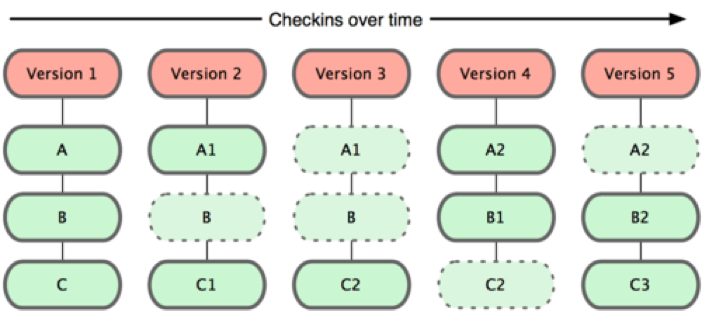
\includegraphics[width=125mm,scale=1]{Figuras/tecnologias/git_over_time}
\caption{Flujo de versiones de Git \citep{chacon2014pro}.}
  \label{graph_git}
\end{figure}

Uno de los fuertes importantes de Git como VCS\footnote{de sus siglas en inglés, Version Control System, que significa en español sistema de control de versionamiento.} es su integridad, debido a que toda versión es verificada mediante una suma de comprobación\footnote{También conocida como checksum.} antes de ser almacenada, y es identificada a partir de ese momento dicha suma. Esta suma es utilizada para volver a un estado anterior del repositorio en caso de ser necesario o ver cuáles fueron los cambios que se realizaron en la porción de código trabajado o más conocido como commit \citep{chacon2014pro}.

\subsection{Spring}
El AMS cuenta con un framework propio desarrollado internamente, el cual esta deprecado y uno nuevo en el cual se estuvo trabajando para los nuevos módulos que se fueron desarrollando. El mismo es Spring MVC y fue utilizado para la parte lógica de la aplicación.

Spring es un framework que facilita el desarrollo de aplicaciones escritas en Java. El propósito de Spring es manejar la infraestructura de las aplicaciones utilizando el método de inversión de control. Es por ello, que el programador se encargará de programar la lógica de negocio usando objetos simples de Java o POJOs (Plain Old Java Objets) y Spring se encargará de añadir las capacidades de empresa o J2EE a la aplicación \citep{bauer2005hibernate}.

Spring tiene las siguientes características:
\begin{itemize}
	\item Simplicidad y acoplamiento débil donde permite programar Java de manera sencilla. Busca ser simple y se basa en la inyección de dependencias para obtener un acoplamiento débil.
	\item Funciona como contenedor ya que gestiona el ciclo de vida de los objetos y como se relacionan entre ellos. Proporciona una gran infraestructura que permite que el programador se dedique a la lógica de la aplicación.
	\item Ligero porque es muy rápido en tiempo de procesamiento y no es invasivo a la hora de programar.
	\item Orientado a aspectos, lo que permite facilitar una capa de servicios que son ideales para este tipo de programación como auditoría, o gestión de transacciones.
\end{itemize} 

Spring se utiliza en el proyecto como framework para toda la aplicación, por lo tanto, usar Spring es también un requerimiento no funcional.

\subsection{AngularJS}
Para empezar a trabajar con la interfaz de usuario se hizo un análisis previo de las ventajas entre Frameworks como JQuery y AngularJS, debido a que la organización que brinda el AMS dio total libertad a la hora de elegir cual utilizar. Por lo tanto, la elección del framework Javascript del módulo de Curriculum entra como decisión de diseño para el proyecto final. 

Con la llegada de los framework de Javascript, tales como JQuery, las páginas web ya no tenían la necesidad de volver a renderizar las páginas cada vez que se necesitaba información del servidor, ya que con la aparición de las llamadas asíncronas se ha logrado mejorar la experiencia del usuario \citep{ruebbelke2015angularjs}.

JQuery ha hecho un excepcional trabajo al proveer de herramientas que manipulen el DOM de una página, pero no ofrece una guía real de cómo organizar el código en la estructura de la aplicación. Ante la desesperada búsqueda de escribir aplicaciones grandes y fáciles de mantener en Javascript ha dado a luz a un renacimiento de frameworks de Javascript, entre ellos se encuentra el framework de Google más conocida como AngularJS.

AngularJS es un framework de aplicaciones web de código abierto que ofrece a un desarrollador una base estable de código con una comunidad enorme y un entorno rico de librerías hechas por la comunidad \citep{darwin2013angularjs}.
\section{Proceso de desarrollo}
El módulo como proyecto de desarrollo enfocado a la metodología Ágil se encuentra dividido en varias épicas para partir en las funcionalidades.

Una épica se encuentra dividida en varias historias de usuario (Figura \ref{epic}), donde las historias de usuario tienen el propósito de entregar valores de negocio al cliente en un periodo establecido de 2 semanas como sprint. Estas historias de usuario pueden ser a la vez divididas buscando la simplicidad de las historias donde cada una debe seguir la práctica INVEST de la metodología Ágil.

Cada historia puede estar compuesta de tareas que tienen como propósito servir al desarrollador como recordatorio de algunas labores pendientes a la hora de desarrollar la historia. Cada tarea debía tener un encargado, pero eso no significaba que esa persona debía hacer sola la implementación.

\begin{figure}[H]
\centering
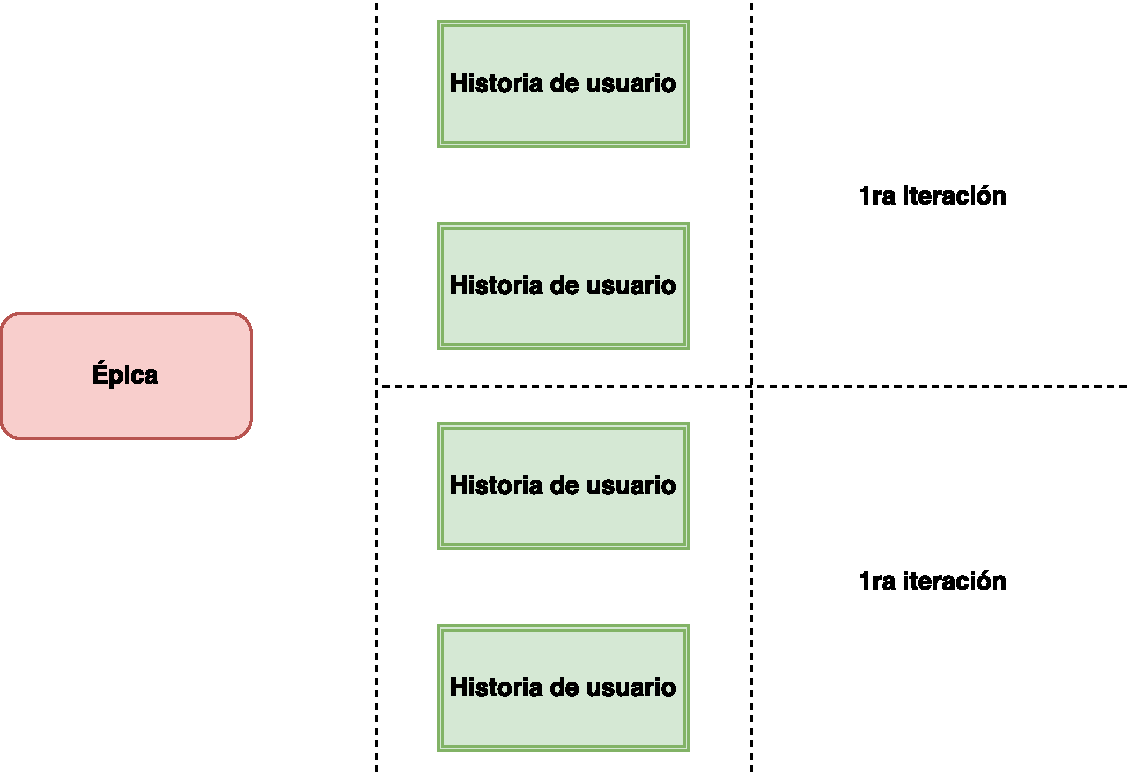
\includegraphics[width=125mm,scale=1]{Capitulos/PropuestadeSolucion/Imagenes/epic_diagram}
\caption{Diagrama de definición de épicas en la metodología ágil}
  \label{epic}
\end{figure}

El PO\footnote{de sus siglas en inglés, Product Owner, que significa en español dueño del producto.} se encarga de la creación de épicas e historias de usuario, en caso de que la historia sea muy grande para terminar en un solo sprint o iteración se vuelve a partir en historias más pequeñas. 

En el caso de estudio, cada sprint consta de 2 semanas de trabajo, donde los desarrolladores como equipo se comprometen a entregar cierto valor de negocio que ellos estiman poder terminar en dicho periodo. Sin embargo, en caso de que el equipo considere que la totalidad de historias no podrán ser entregadas antes de que termine el periodo se pasa al siguiente sprint o se achica la historia minimizando los criterios de aceptación y los restantes se agregan en otra historia de usuario para las siguientes iteraciones.

Cada equipo tiene un líder, donde cada líder tiene como rol ser la brecha que une al PO con los desarrolladores. El PO se reúne con el líder de cada equipo para verificar las prioridades de las historias de usuario que están pendientes en el backlog\footnote{Bolsa de historias de usuarios pendientes.}. 

Al inicio del diseño de la aplicación se llevará a cabo una serie de diseños de funcionalidad y usabilidad que llevar a la mejor experiencia de uso del módulo de gestión curricular, donde dichos diseños serán validados por el equipo en los Estados Unidos antes de iniciar el desarrollo.

\subsection{Scrum}
Scrum es un proceso en el que se aplican de manera regular un conjunto de prácticas para trabajar colaborativamente, en equipo, y obtener el mejor resultado posible de un proyecto. Estas prácticas se apoyan unas a otras y su selección tiene origen en un estudio de la manera de trabajar de varios equipos altamente productivos.

En Scrum se realizan entregas parciales y regulares del producto final, priorizadas por el beneficio que aportan al PO. Por ello, Scrum está especialmente indicado para proyectos en entornos complejos donde se necesita obtener resultados con el mínimo esfuerzo y los requisitos son cambiantes o poco definidos. Además, en dichos ambientes la innovación, la competitividad, la flexibilidad, y la productividad son fundamentales.

Scrum también se utiliza para resolver situaciones en que no se está entregando al cliente lo que necesita, cuando las entregas se alargan demasiado, los costes se disparan o la calidad no es aceptable, cuando se necesita capacidad de reacción ante la competencia, cuando la moral de los equipos es baja y la rotación alta, cuando es necesario identificar y solucionar ineficiencias sistemáticamente o cuando se quiere trabajar utilizando un proceso especializado en el desarrollo de producto. 

\subsection{Proceso}
En Scrum un proyecto se ejecuta en bloques temporales cortos y fijos que los conocemos como sprints o iteraciones. Estas iteraciones por lo general duran 2 semanas aunque en algunos equipos son de 3 y hasta 4 semanas, límite máximo de feedback y reflexión\citep{davis_agile_2015}. Cada iteración tiene que proporcionar un resultado completo, un incremento de producto final que sea susceptible de ser entregado con el mínimo esfuerzo al cliente cuando lo solicite.

El proceso parte de la lista de objetivos o requisitos priorizada del producto, que actúa como plan del proyecto. En esta lista el cliente prioriza los objetivos balanceando el valor que le aportan respecto a su coste y quedan repartidos en sprints y entregas.

\begin{figure}[H]
\centering
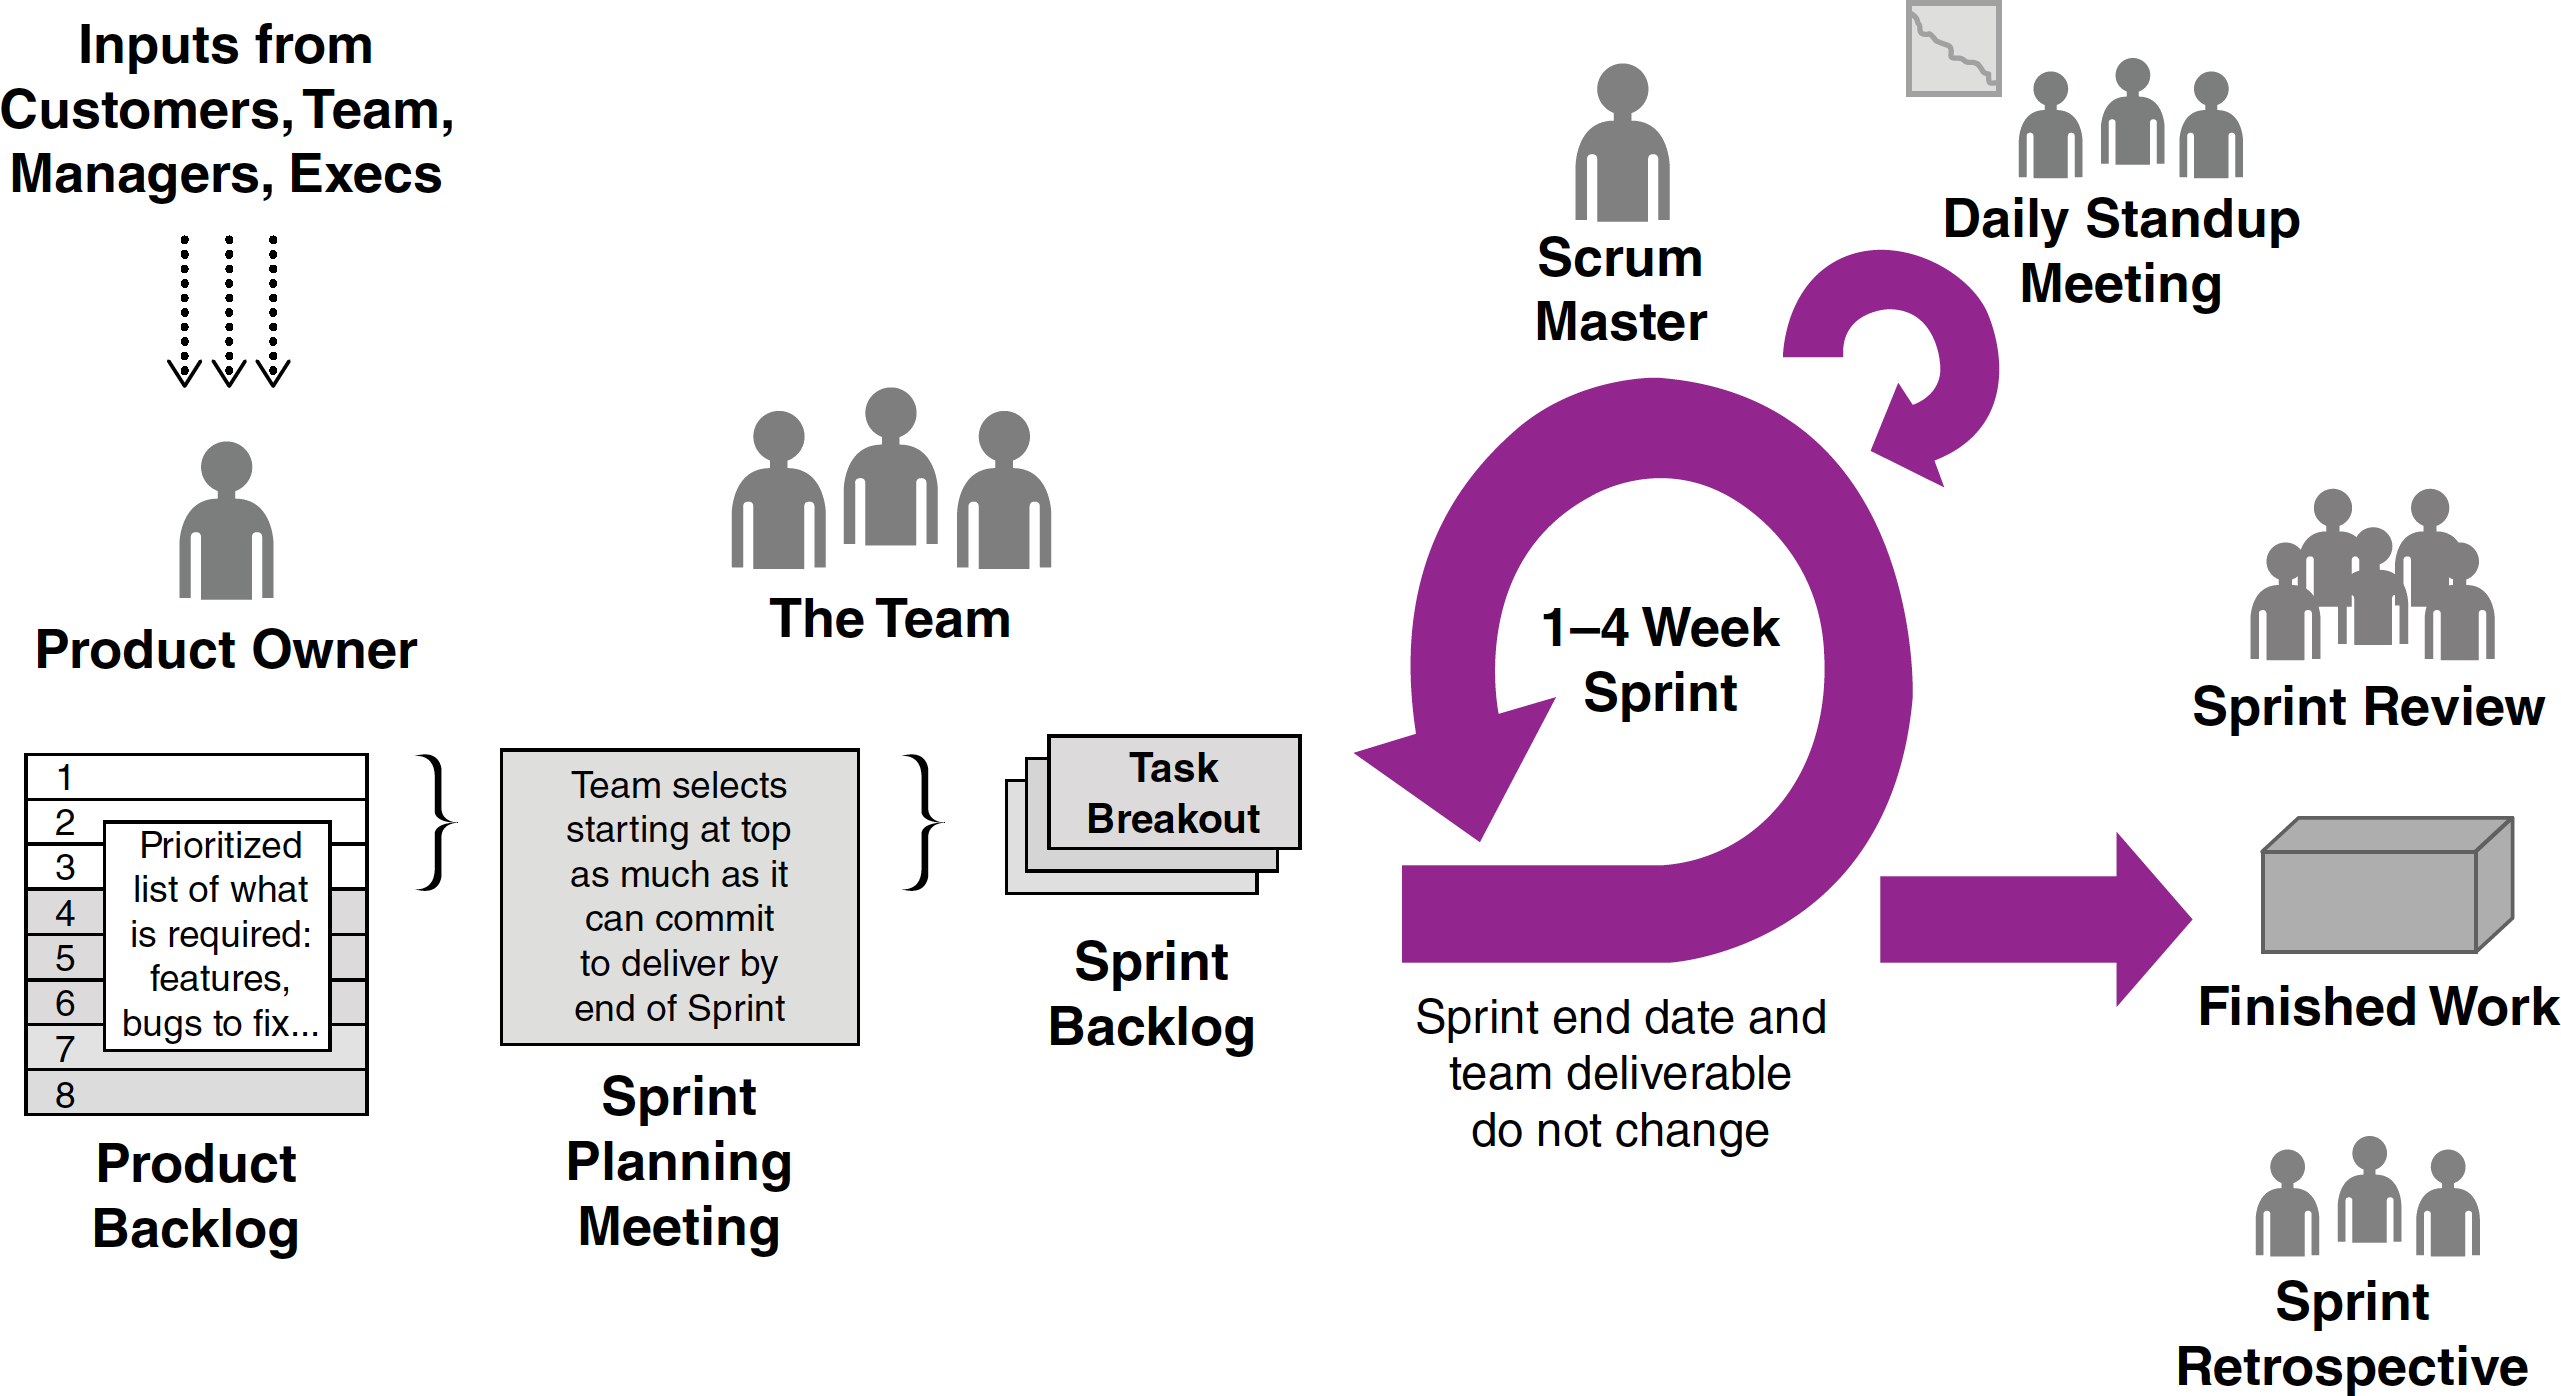
\includegraphics[width=125mm,scale=1]{Figuras/flujo_scrum}
\caption{Flujo de la técnica SCRUM\citep{cobb2015project}.}
  \label{flujo_scrum}
\end{figure}

\subsection{Planificación de iteraciones}
El primer día de la iteración se realiza la reunión de planificación de la iteración y consta de dos partes:
\begin{itemize}
    \item \textbf{Selección de requisitos} (4 horas máximo) – El PO presenta al equipo la lista de requisitos priorizada del producto o proyecto. El equipo pregunta al PO las dudas que surgen y selecciona los requisitos prioritarios que se compromete a completar en la iteración, de manera que puedan ser entregados en caso de ser solicitados.
    \item \textbf{Planificación de la iteración o sprint} (4 horas máximo) – El equipo elabora la lista de tareas de la iteración necesarias para desarrollar los requisitos a que se ha comprometido. La estimación de esfuerzo se hace de manera conjunta y los miembros del equipo se asignan las tareas.
\end{itemize}

\subsection{Ejecución del Sprint}
El equipo realiza una reunión diaria (15 minutos aproximadamente). Cada miembro del equipo inspecciona el trabajo que el resto está realizando (dependencias entre tareas, progreso hacia el objetivo de la iteración, obstáculos que pueden impedir este objetivo) para poder hacer las adaptaciones necesarias que permitan cumplir con el compromiso adquirido. En la reunión cada miembro del equipo responde a tres preguntas:
\begin{itemize}
    \item ¿Qué he hecho desde la última reunión diaria?
    \item ¿Qué voy a hacer a partir de este momento?
    \item ¿Qué impedimentos tengo o voy a tener?
\end{itemize}
Durante la iteración el Scrum Master se encarga de que el equipo pueda cumplir con su compromiso y de que no se merme la productividad del equipo. Además, elimina los obstáculos que el equipo no puede resolver por sí mismo.

Durante el sprint, el PO junto con el equipo refinen la lista de requisitos para prepararlos para los siguientes sprints y, si es necesario, cambian o vuelven a planificar los objetivos del proyecto para maximizar la utilidad de lo que se desarrolla y el retorno de inversión.

\subsection{Inspección y adaptación}
El último día de la iteración se realiza la reunión de revisión del sprint la cual consta de dos partes:
\begin{itemize}
    \item \textbf{Demostración} (3 horas aproximadamente) – El equipo presenta al PO los requisitos completados en la iteración, en forma de incremento de producto preparado para ser entregado con el mínimo esfuerzo. En función de los resultados mostrados y de los cambios ocurridos en el contexto del proyecto, el PO realiza las adaptaciones necesarias de manera objetiva, ya desde la primera iteración, volviendo a planificar el proyecto.
    \item \textbf{Retrospectiva} (1 hora) - El equipo analiza cómo ha sido su manera de trabajar y cuáles son los problemas que podrían impedirle progresar adecuadamente, mejorando de manera continua su productividad. El Scrum Master se encargará de ir eliminando los obstáculos identificados.
\end{itemize}

% DISEÑO Y DESARROLLO DE LA APLICACION
\chapter{Desarrollo de la aplicación} % Main chapter title
\label{capitulo5} % Change X to a consecutive number; for referencing this chapter elsewhere, use \ref{capitulo6}
En este capítulo presentamos el proceso de desarrollo del módulo de gestión de programas orientado a competencias. Comenzamos listando las épicas y brindando una breve explicación de cada una de ellas.

La validación de las historias de usuario desarrolladas es de particular importancia. Si bien la validación se realizó de manera iterativa al final de los sprints, las presentamos en este escrito aparte, en el capítulo \ref{capitulo7}.

\subsection*{Épicas}
\begin{enumerate}
	\item Análisis de herramientas utilizadas y posibles potenciales para el desarrollo del módulo.
	\item Diseño de modelo de datos para versionamiento de competencias, cursos y programas.
	\item Desarrollo de flujo de trabajo para el versionamiento de competencias.
	\item Desarrollo de buzón de entrada para evaluadores y colaboradores del flujo de trabajo.
	\item Versionamiento encadenado de evaluaciones debido al versionamiento de competencias.
	\item Desarrollo de flujo de trabajo para el versionamiento de cursos.
	\item Desarrollo de flujo de trabajo para el versionamiento de programas de estudio.
 	\item Soporte de etapas en los flujos de trabajo.
	\item Desarrollo de reportes de versiones de cursos.
	\item Actualizar el AMS para que tome las versiones de competencias cursos y programas correspondientes en los periodos.
	\item Retoques finales.
\end{enumerate}

\resizebox{\columnwidth}{!}{%
\begin{ganttchart}[vgrid, hgrid, bar height=0.7, y unit chart=0.5cm, progress=today, today=24, bar label text={#1$\rightarrow$}, progress label text={#1$\%$}, today label=HOY]{1}{26}
\gantttitle{2016}{12}
\gantttitle{2017}{14} \ganttnewline
\gantttitle{Jul}{2}
\gantttitle{Ago}{2}
\gantttitle{Set}{2}
\gantttitle{Oct}{2}
\gantttitle{Nov}{2}
\gantttitle{Dic}{2}
\gantttitle{Ene}{2}
\gantttitle{Feb}{2}
\gantttitle{Mar}{2}
\gantttitle{Abr}{2}
\gantttitle{May}{2}
\gantttitle{Jun}{2} 
\gantttitle{Jul}{2} \\
\ganttbar[progress=100]{1}{1}{1} \\
\ganttbar[progress=100]{2}{2}{2} \\
\ganttbar[progress=100]{3}{3}{6} \\
\ganttbar[progress=100]{4}{5}{10} \\
\ganttbar[progress=100]{5}{11}{16} \\
\ganttbar[progress=100]{6}{11}{23} \\
\ganttbar[progress=100]{7}{13}{21} \\
\ganttbar[progress=100]{8}{23}{24} \\
\ganttbar[progress=100]{9}{22}{23} \\
\ganttbar[progress=100]{10}{22}{23} 
\end{ganttchart}
}


\section{Análisis de herramientas}
La primera etapa del proyecto fue realizar una encuesta a los posibles integrantes del nuevo equipo de desarrollo donde se verifican las capacidades adquiridas en cuanto a lenguajes de programación y tecnologías utilizadas, como así también de los conocimientos de dominio de la aplicación.
Dicha encuesta tiene como propósito permitir una mejor organización de los miembros de equipos y de esta manera una distribución eficaz de conocimientos y dominio de la aplicación para resolver las diferentes problemáticas que podría afectar al módulo currilar.
Una vez formado lo que sería el equipo de desarrollo se procedió a hacer análisis de las herramientas que podrían resolver la problemática entre ellas las que eran tomadas como requerimientos no funcionales para el módulo de gestión curricular del capítulo \ref{reqnofuncional}.
\section{Diseño de modelo de datos para versionamiento}
\subsection{Diseño del modelo de versionamiento para competencias, cursos y programas}
Al iniciar con las historias de versionamiento, se definió una tarea en la cual participaron algunos miembros de equipo y tenía como propósito principal el diseño de una lógica de negocios que permita adaptar las tablas existentes de las competencias, evaluaciones, cursos, y programas para que soporten una revisión o versionamiento de sus registros.

Como resúmen de actividades del modelo desarrollado (figura \ref{version_model}) se puede resaltar lo siguiente:
\begin{itemize}
	\item Cada tabla de cualquier entidad posee un identificador único. Las tablas entidades versionables son las de competencias, cursos, programas, y evaluaciones.
	\item Se decidió agregar una nueva columna \enquote{entity_atid} que tiene como propósito el de apuntar al origen de la versión. Por ejemplo; si el usuario crea un nuevo curso para el año lectivo, este curso tiene su identificador \enquote{course_id} y su \enquote{course_atid} apuntando a su mismo identificador por ser el origen para las versiones posteriores. Luego, se crea una nueva versión para el año posterior, esta nueva versión tiene su propio identificador pero su campo denominado como \enquote{course_atid} que apunta al primer curso creado u origen.
	\item Para hacer más sencilla la búsqueda de competencias, cursos, programas o evaluaciones actuales se agregó un campo a cada tabla identificando los actuales. Este campo denominado \enquote{is_current} o “es actual” es una bandera que indica la validez del registro.
	\item Además de registrar el origen, se registra la versión previa o de donde parte el registro con el campo \enquote{previous_entity_id}.
	\item Como cada registro de cualquier tabla ahora tiene un periodo de validez, se diseñaron tablas de relación entre cada tabla y la tabla de periodos lectivos denominada como \enquote{calendar}. Por ejemplo; \enquote{slo_term_rel} para las competencias, \enquote{new_course_term_rel} para los cursos, \enquote{asmt_term_rel} para las evaluaciones y \enquote{credential_term_rel} para los programas.
\end{itemize}

\begin{figure}
\centering
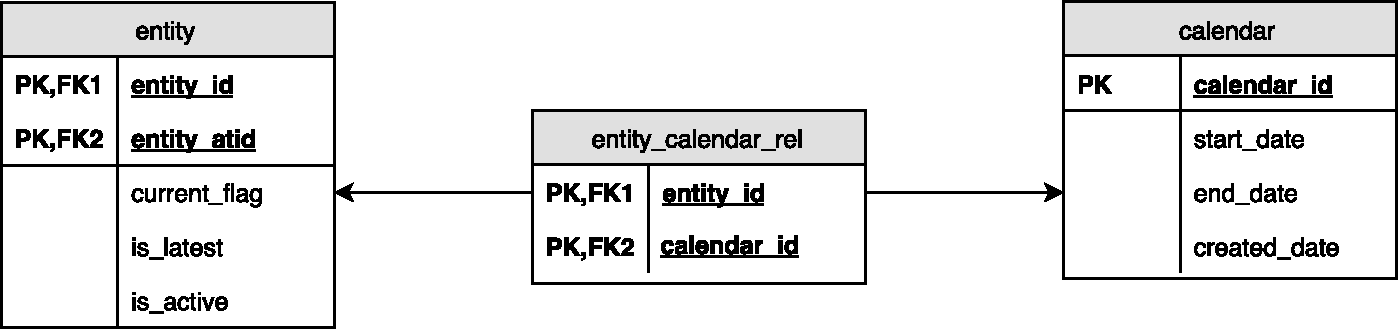
\includegraphics[width=125mm,scale=1]{Capitulos/DesarrollodelaAplicacion/Imagenes/version_model}
\caption{Modelo de datos para el versionamiento de competencias, cursos y programas.}
  \label{version_model}
\end{figure}
\section{Flujo de trabajo para el versionamiento de competencias}
\subsection{Versionamiento de competencias}
Esta historia de usuario tenía como descripción los siguiente \enquote{Como encargado del sistema de gestión de competencias, me gustaría ser capaz de versionar competencias con la finalidad de que se puedan redefinir competencias con el paso del tiempo, sin perder datos de corrección de las mismas}.

Algunas tareas que se definieron en la historia de usuario son las siguientes:
\begin{itemize}
	\item Investigar y diseñar el versionamiento de las competencias. La misma fue desarrollada de manera en que toda competencia versionada apunta al origen y el origen se apunta a sí mismo, de esta manera se puede saber la familia de versiones de una competencia.
	\item Actualizar todos esos lugares de la aplicación que listan las competencias, donde solamente deberían traer las competencias actuales.
	\item Manejar la distribución de competencias a periodos futuros, de manera que una competencia no pueda ser distribuida a periodos en las que no tiene validez.
	\item Diseñar y mantener pruebas automatizadas con Selenium.
\end{itemize}

Fue desarrollado durante tres iteraciones con un total de 170 horas cargadas en el sistema, debido a la complejidad a la hora de migrar los datos ya existentes de todas las universidades y por la cantidad de servicios que debían ser modificados.

\subsection{Flujo de trabajo simple}
En la siguiente historia de usuario inicia el proceso de creación de flujos de trabajo donde las plantillas de los flujos de trabajo pueden ser creados, editados y eliminados por el administrador encargado de la aplicación de cada universidad. Para esta historia se debe diseñar y desarrollar las plantillas de manera que el administrador pueda agregar los diferentes pasos del flujo de trabajo si así lo decide en el futuro. Inicialmente se considera un solo paso para la iteración inicial de desarrollo.

Esta historia de usuario tenía como descripción los siguiente \enquote{Como coordinador del AMS, me gustaría ser capaz de crear flujos de trabajo simples para administrar la aprobación de revisiones de competencias y que se pueda tener un mejor manejo de las creaciones y aprobaciones de las mismas en el campus}.

La historia tiene los siguientes criterios de aceptación:
\begin{itemize}
	\item Diseñar e implementar plantillas de flujo de trabajos simples para creación y revisión de todos los niveles de competencias.
	\item Diseñar e implementar un flujo de trabajo simple sin aprobación por parte de evaluadores, donde el iniciador del flujo puede revisar y aprobar su propio formulario.
	\item La plantilla de flujo de trabajo simple debe soportar el uso de pasos personalizados.
	\item El que inició el flujo es el único que puede llenar los campos del formulario.
\end{itemize}

El usuario debe ser capaz de agregar pasos personalizados para la plantilla de flujo de trabajo de la institución. Estos pasos personalizados son pasos que puede diseñar el usuario, donde puede colocar una pregunta como título y por cada título tiene un campo que puede llenar el usuario. Por lo general, un paso personalizado puede tener una o más preguntas definida por el usuario.

En los mockups entregados para el desarrollo se contemplan trabajos futuros donde cada paso tiene que ser aprobado por un rol del AMS, donde cualquier usuario con dicho rol puede aprobar o rechazar el flujo de trabajo con solo rechazar uno de los pasos. 

Además, se da inicio al desarrollo de plantillas de flujos de trabajo con las competencias, donde se podía asignar un tipo de flujo para cada plantilla ya sea de creación o versionamiento de los diferentes niveles de competencias.

Como las plantillas era una funcionalidad conocida y utilizada en otra parte de la aplicación, se imitó el comportamiento de la misma utilizando las mismas tablas para el almacenamiento de los datos en la base de datos relacional como requisito no funcional de la organización. Se diseñaron las nuevas pantallas con la definición de las plantillas de flujo de trabajo y también la pantalla para listar las mismas. En la misma el usuario administrador puede crear, editar si aún no ha sido usada, eliminar y clonar plantillas.

La historia de usuario fue desarrollada durante una iteración con un total de 90 horas cargadas en el sistema.

\subsection{Aprobación de pasos completados del flujo de trabajo para competencias}

Luego de la historia de diseño de las plantillas y un flujo de trabajo simple para creación o versionamiento de competencias, el siguiente paso es que un usuario designado desde la plantilla pueda iniciar y otro pueda aprobar el proceso de creación o revisión de competencias de cualquier nivel.

Esta historia de usuario tenía como descripción los siguiente \enquote{Como evaluador de un flujo de trabajo, me gustaría un simple proceso paso por paso para que pueda revisar y/o aprobar competencias de manera sencilla e intuitiva}.

La historia de usuario tiene los siguientes criterios de aceptación:
\begin{itemize}
	\item Soporte de asignaciones de tareas de creación y revisión por roles del AMS en las plantillas de flujos de trabajo.
	\item Diseño e implementación de vista de revisión para el flujo de trabajo.
\end{itemize}

Cada paso del flujo de trabajo debe estar terminado para que pase a la etapa de revisión por parte de los encargados. Luego de enviar el formulario, cada rol debe hacer su revisión para que el sistema pueda agregar la nueva competencia.

Como en las reuniones de demostración de cada sprint se notaban ciertos aspectos de las historias de usuario que no llenaban las expectativas de los clientes, los desarrolladores decidieron diseñar maquetas de pantallas que mostraban el posible diseño de la página. Luego de recibir feedback de parte de los clientes, se empezaba a desarrollar las nuevas pantallas. Finalizando la historia de usuario con pruebas automatizadas.

La historia de usuario fue desarrollada durante una iteración en un periodo de tiempo de 44 horas cargadas en el sistema.

\subsection{Rechazar pasos completados del flujo de trabajo}
Esta historia de usuario tenía como descripción los siguiente \enquote{Como evaluador de flujos de trabajo, me gustaría ser capaz de rechazar partes de los mismos y poder dar feedback a partes que no cumplen con nuestros estándares}.

\begin{itemize}
	\item Diseño e implementación de funcionalidad de rechazo de pasos en los flujos de trabajo.
	\item Diseño e implementación de funcionalidad de retroalimentación de parte de los evaluadores y encargados.
\end{itemize}

Esta funcionalidad tiene como propósito permitir a la persona que hace la revisión de los pasos rechazar y dejar feedback para que se puedan hacer los cambios correspondientes. Cuando se rechaza un paso, se rechaza el flujo de trabajo, y por lo tanto vuelven a estar activos los campos para que se hagan los cambios correspondientes.

El trabajo se inició la actualización del modelo de base de datos actual, luego de crear las clases correspondientes en el código para su utilización. Luego, se actualizaron las páginas donde el usuario puede aprobar los steps para que soporte rechazar pasos y poder así dejar algunos comentarios. 

La historia de usuario fue desarrollada durante una iteración en un periodo de tiempo de 53 horas cargadas en el sistema.

\section{Buzón de entrada para evaluadores y colaboradores del flujo de trabajo}
\subsection{Buzón de entradas de flujos de trabajo}
La siguiente historia tiene como propósito mostrar a cada usuario la lista de workflows pendientes que requiere de su aporte. Además de adaptar el nuevo buzón de entrada para otros rasgos de la aplicación como son las evaluaciones, los planes de acción y preguntas de parte del usuario a profesores.

Tiene como descripción lo siguiente \enquote{\textit{Como aprobador de eLumen, me gustaría una vista unificada de los workflows que tengo que revisar – además de mis evaluaciones, planes de acción y mis preguntas a profesores – para que no vaya cazando workflows por la aplicación}}

Como criterios de aceptación se encuentran los siguientes:
\begin{itemize}
	\item Diseño e implementación de buzón de entrada para flujos de trabajo.
	\item Diseño e implementación de buzón de entrada para planes de acción.
	\item Diseño e implementación de buzón de entrada para pedidos de profesores.
\end{itemize}

La historia fue finalizada en dos iteraciones con una cantidad de 56 horas cargadas en el sistema.

\subsection{Notificaciones con soporte a etapas}
La historia de usuario tiene como descripción lo siguiente \enquote{\textit{Como presidente curricular, me gustaría que el equipo de diseño y revisión curricular reciban notificaciones cuando tengan alertas de deuda de trabajo (y alertas cuando pase el tiempo), para que se puedan manejar mejor de esa manera los procesos curriculares}}.

Como criterios de aceptación se encuentran los siguientes:
\begin{itemize}
	\item Establecer notificaciones cuando las partes del flujo de trabajo son asignadas a los roles de las personas.
	\item Establecer notificaciones de alerta a asignaciones de partes y etapas. Por ejemplo, 5 días después de su asignación.
	\item Mandar notificaciones por mail.
\end{itemize}

Algunas de las tareas identificadas en la planificación de las iteraciones eran los siguientes:
\begin{itemize}
	\item Diseñar e implementar nuevos modelos de datos que permitan soportar el uso de roles para creadores y editores de partes.
	\item Actualizar el sistema de notificaciones del AMS.
	\item Diseñar e implementar la página de configuración de notificaciones.
\end{itemize}

La historia fue finalizada en tres iteraciones con una cantidad de 60 horas cargadas en el sistema.
\section{Versionamiento de evaluaciones}
La épica fue creada para abarcar todos los cambios que requerían las evaluaciones en sus diferentes formas de versionamiento. Entre ellas, se encuentra el versionamiento encadenado de las evaluaciones debido al flujo terminado de versionamiento de competencias. 

En caso de que existan evaluaciones ya creadas para las secciones de los cursos y en dicho curso se generaba una nueva versión de alguna de sus competencias, el sistema debía versionar las evaluaciones que utilizaba la versión anterior de dicha competencia con la versión actual para el periodo.

Como trabajo futuro se cuenta con el desarrollo de flujos de trabajo para las evaluaciones, ya que el versionamiento que ahora cuenta el sistema es automático y no a través de formularios web.

\begin{table}[H]
\centering
\resizebox{\columnwidth}{!}{%
\begin{tabular}{@{}lllll@{}}
\toprule
Historias de usuario           & HE & HC & PH &  Sprints \\ \midrule
Versionamiento de evaluaciones & 102 & 87 & 8 &  2 \\ \bottomrule
\end{tabular}
}
\caption{Historias de usuario para el versionamiento encadenado de evaluaciones debido al versionamiento de competencias}
\label{epic:5}
\end{table}

\subsection{Versionamiento de evaluaciones} \label{versionamiento_encadenado}
La historia de versionamiento de evaluaciones tiene como propósito permitir el versionamiento automático de evaluaciones existentes que utilizar competencias del sistema. Por ejemplo, en caso de que una evaluación hecha por un profesor tenga una nueva versión en el nuevo periodo de su sección, el sistema versiona la evaluación para ese periodo obteniendo las competencias actuales.

La historia de usuario tiene como descripción: \enquote{\textit{Como usuario del módulo curricular, me gustaría ser capaz de versionar mis evaluaciones, para que se observen los cambios a través del tiempo. Y que la interfaz y los reportes sigan presentando datos para los diseños históricos}}.

Algunas de las tareas fueron las siguientes:
\begin{itemize}
	\item Adaptar versionamiento para el modelo de datos de las evaluaciones.
	\item Migrar datos de los usuarios para que soporten versionamiento de las mismas.
	\item Actualizar el selector de evaluaciones de los profesores para que puedan seleccionar evaluaciones actuales.
	\item Actualizar el widget de profesores que utilizan las evaluaciones como datos.
\end{itemize}

Esta historia de usuario fue realizada en una iteración con un total de 87 horas cargadas en el sistema.

\section{Flujo de trabajo para el versionamiento de cursos}
\begin{table}[H]
\centering
\resizebox{\columnwidth}{!}{%
\begin{tabular}{@{}lllll@{}}
\toprule
Historias de usuario              & HE & HC & PH & Sprints \\ \midrule
Versionamiento de cursos          & 84 & 96 & 13 & 3       \\
Información básica de curso       & 46 & 53 & 5  & 1       \\
Horas y unidades de evaluación    & 48 & 66 & 5  & 1       \\
Especificaciones de curso         & 40 & 40 & 5  & 1       \\
Requisitos de curso               & 44 & 40 & 5  & 1       \\
Revisar y aprobar curso           & 48 & 68 & 5  & 1       \\
Competencias de curso             & 80 & 76 & 8  & 1       \\
Esquema de curso                  & 40 & 48 & 5  & 1       \\
Códigos de clasificación de curso & 56 & 80 & 5  & 1       \\ \bottomrule
\end{tabular}
}
\caption{Historias de usuario para el flujo de trabajo para el versionamiento de cursos}
\label{epic:6}
\end{table}


\subsection{Versionamiento de cursos}
Esta historia de usuario fue realizada en tres iteraciones con un total de 96 horas cargadas, debido a que los cambios que suponía conllevan a una migración importante de datos de los usuarios.

Tenía como descripción: \enquote{\textit{Como coordinador del AMS, me gustaría poder hacer una versión de mi plan de curso para que pueda realizar un seguimiento de los cambios para cosas como la revisión de programas y los acuerdos de articulación y transferencia en la aplicación}}.

Algunas de las tareas realizadas en la historia fueron las siguientes:

\begin{itemize}
	\item Buscar técnicas y herramientas de versionamiento parecidas para implementar.
	\item Diseñar una posible solución a la problemática.
	\item Implementar cambios en la base de datos mediante scripts en el proyecto.
	\item Actualizar clases Java existentes en el proyecto de cursos.
	\item Implementar la solución para el flujo de trabajo.
	\item Actualizar la creación de cursos sin el módulo curricular con los nuevos campos.
	\item Adaptar la relación de cursos y competencias para que soporte el versionamiento de los mismos.
	\item Actualizar la lista de competencias por cursos.
\end{itemize}

\subsection{Información básica de curso}
Esta historia de usuario tiene como propósito de diseñar páginas que permitan al usuario completar la información básica de curso que buscan diseñar, así también fueron proporcionados mockups para la pantalla (figura \ref{course_cover_info}).

Tiene la siguiente descripción: \enquote{\textit{Como miembro del comité de Curriculum, me gustaría ser capaz de administrar la página de información básica de cursos, para que no tenga que buscar por documentos a la hora de crear o versionar cursos}}.

\begin{itemize}
	\item Diseñar un modelo de datos que soporte el nuevo formato de información de curso.
	\item Adaptar tablas existentes y crear clases nuevas para las nuevas entidades de base de datos.
	\item Actualizar la plantilla de creación de Workflow para que soporte el nuevo paso.
	\item Actualizar el visualizador de Workflow.
	\item Diseño de pruebas automatizadas.
\end{itemize}

La historia se terminó en una iteración con un total de 53 horas de desarrollo.

\begin{figure}[H]
\centering
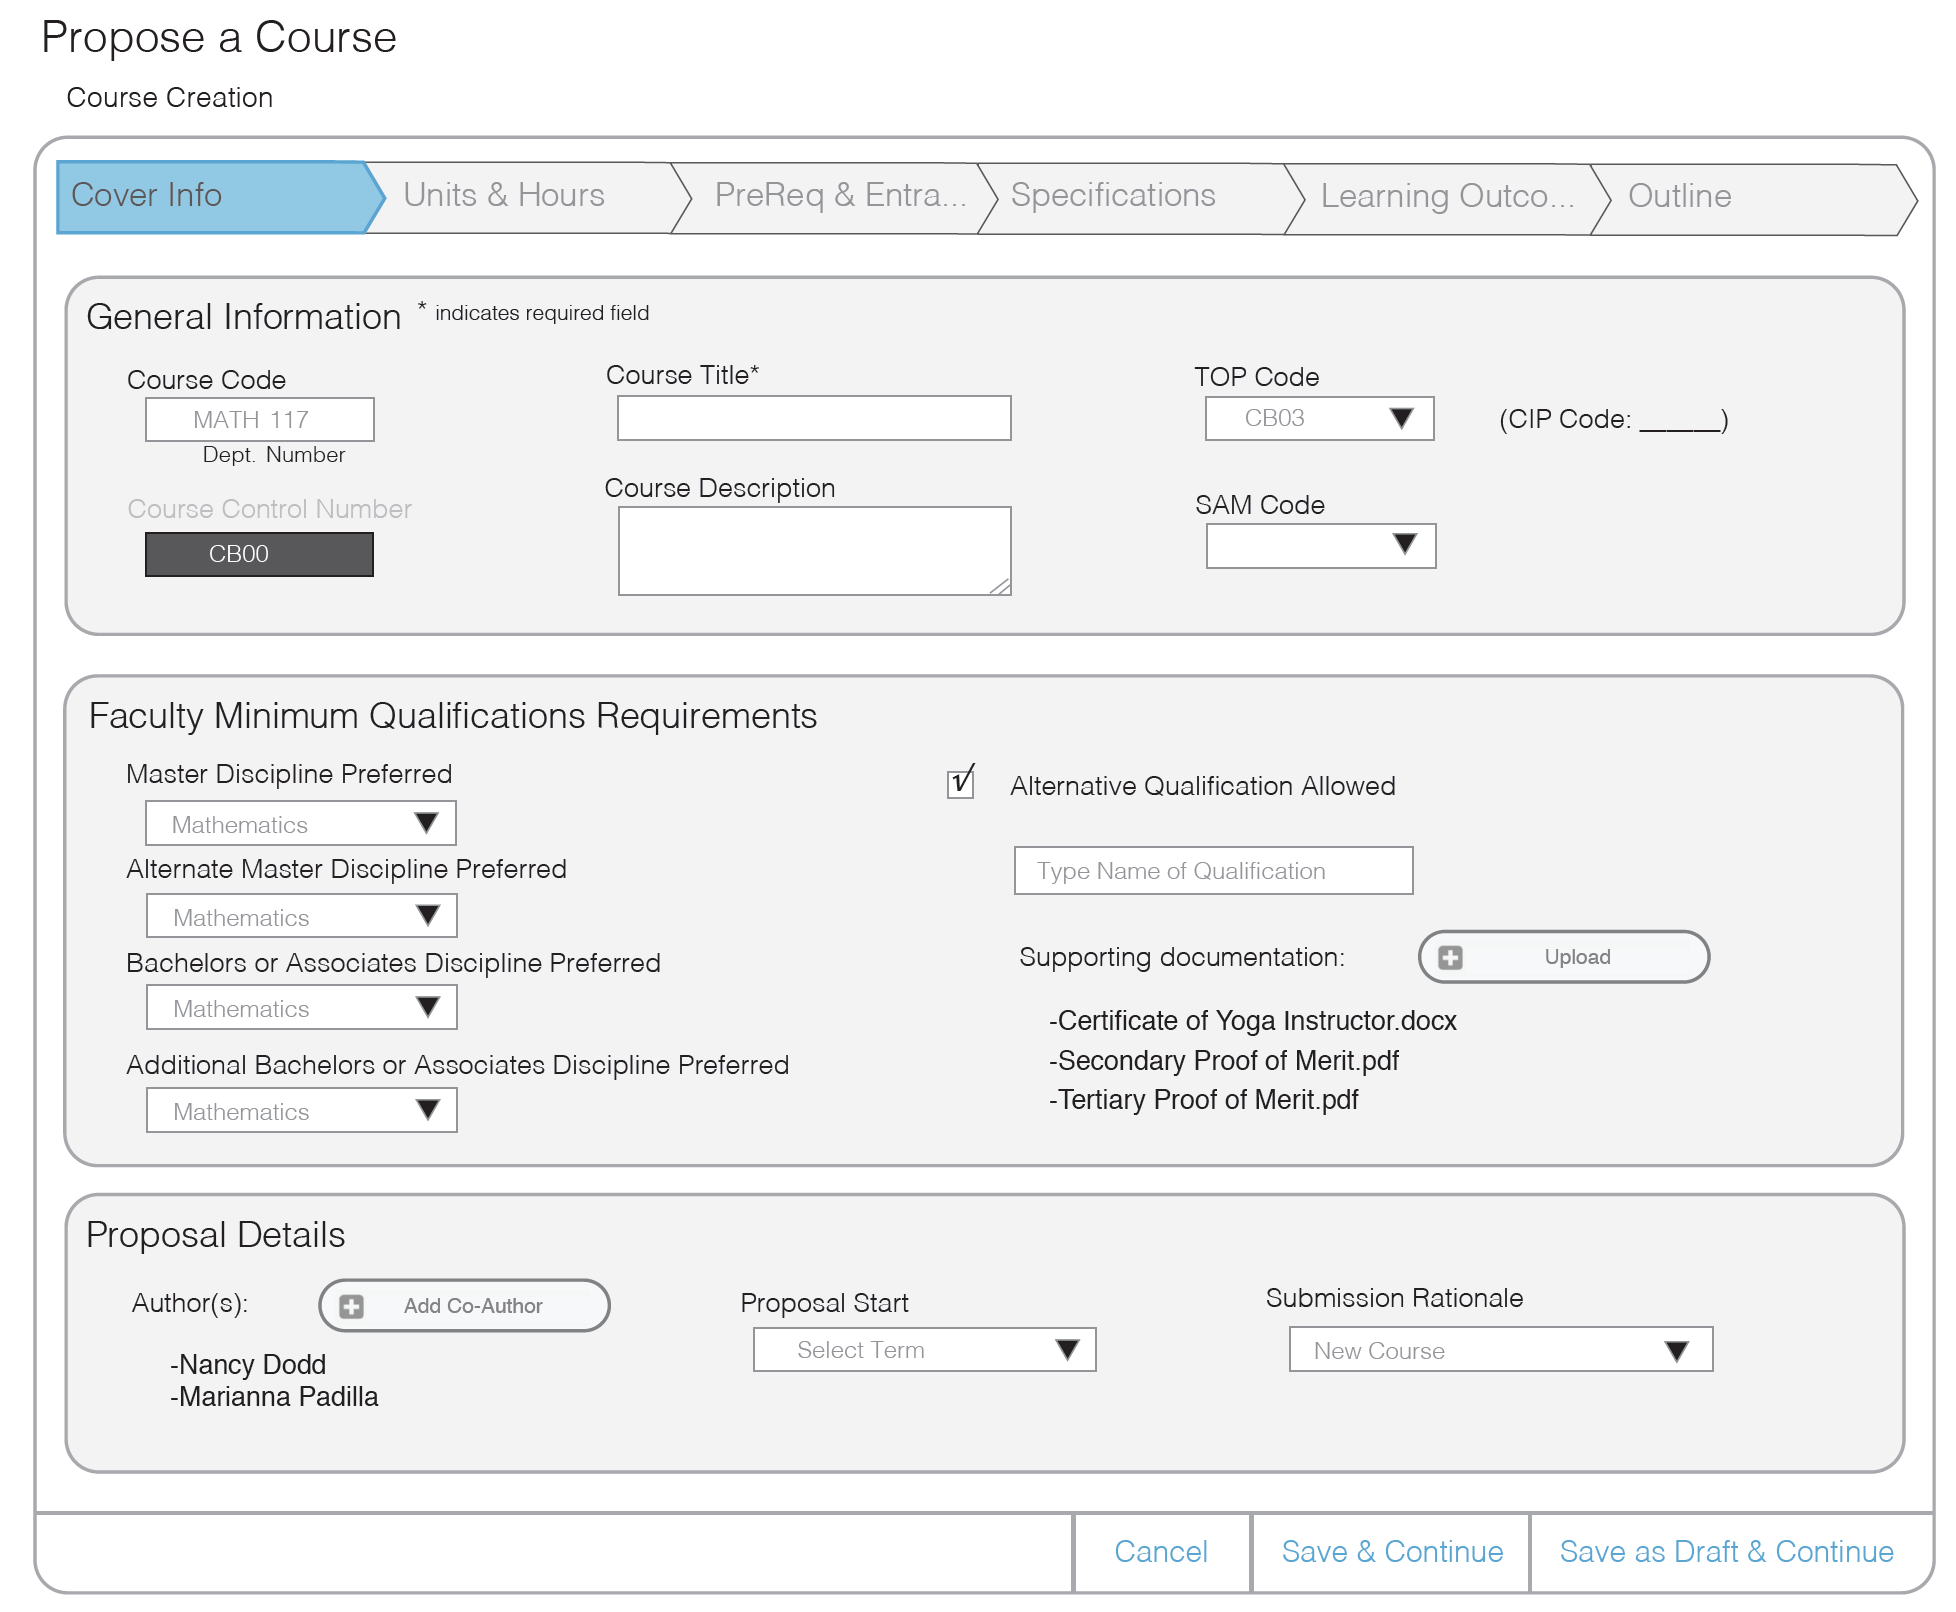
\includegraphics[scale=0.3]{Capitulos/DesarrollodelaAplicacion/Imagenes/course_cover_info}
\caption{Mockup de la pantalla de información básica de curso.}
  \label{course_cover_info}
\end{figure}

\subsection{Horas y unidades de evaluación}
En esta historia se desarrolló un nuevo paso para el desarrollo de flujo de trabajo, en la cual el encargo del mismo va a poder detallar las horas y unidades que requiere el curso o que va a requerir.

La organización ha proveído mockups (figura \ref{course_units_hours}) para la página como criterio de aceptación de la historia es que siga el modelo de la misma.

La historia tenía la siguiente descripción: \enquote{\textit{Como profesor encargado del curso, me gustaría tener una página de horas y métricas para que pueda conseguir información básica sobre mi curso en el AMS}}.

La historia a desarrollar se dividió entre miembros del equipo de desarrollo en las siguientes tareas:
\begin{itemize}
	\item Modificar el modelo de datos para que soporte los nuevos campos de curso.
	\item Crear y/o editar las clases Java.
	\item Actualizar la plantilla de flujo de trabajos.
	\item Actualizar el visualizador de flujo de trabajos.
	\item Pruebas de funcionalidad.
\end{itemize}

La historia ha sido terminada en una iteración con un total de 66 horas de desarrollo.

\begin{figure}[H]
\centering
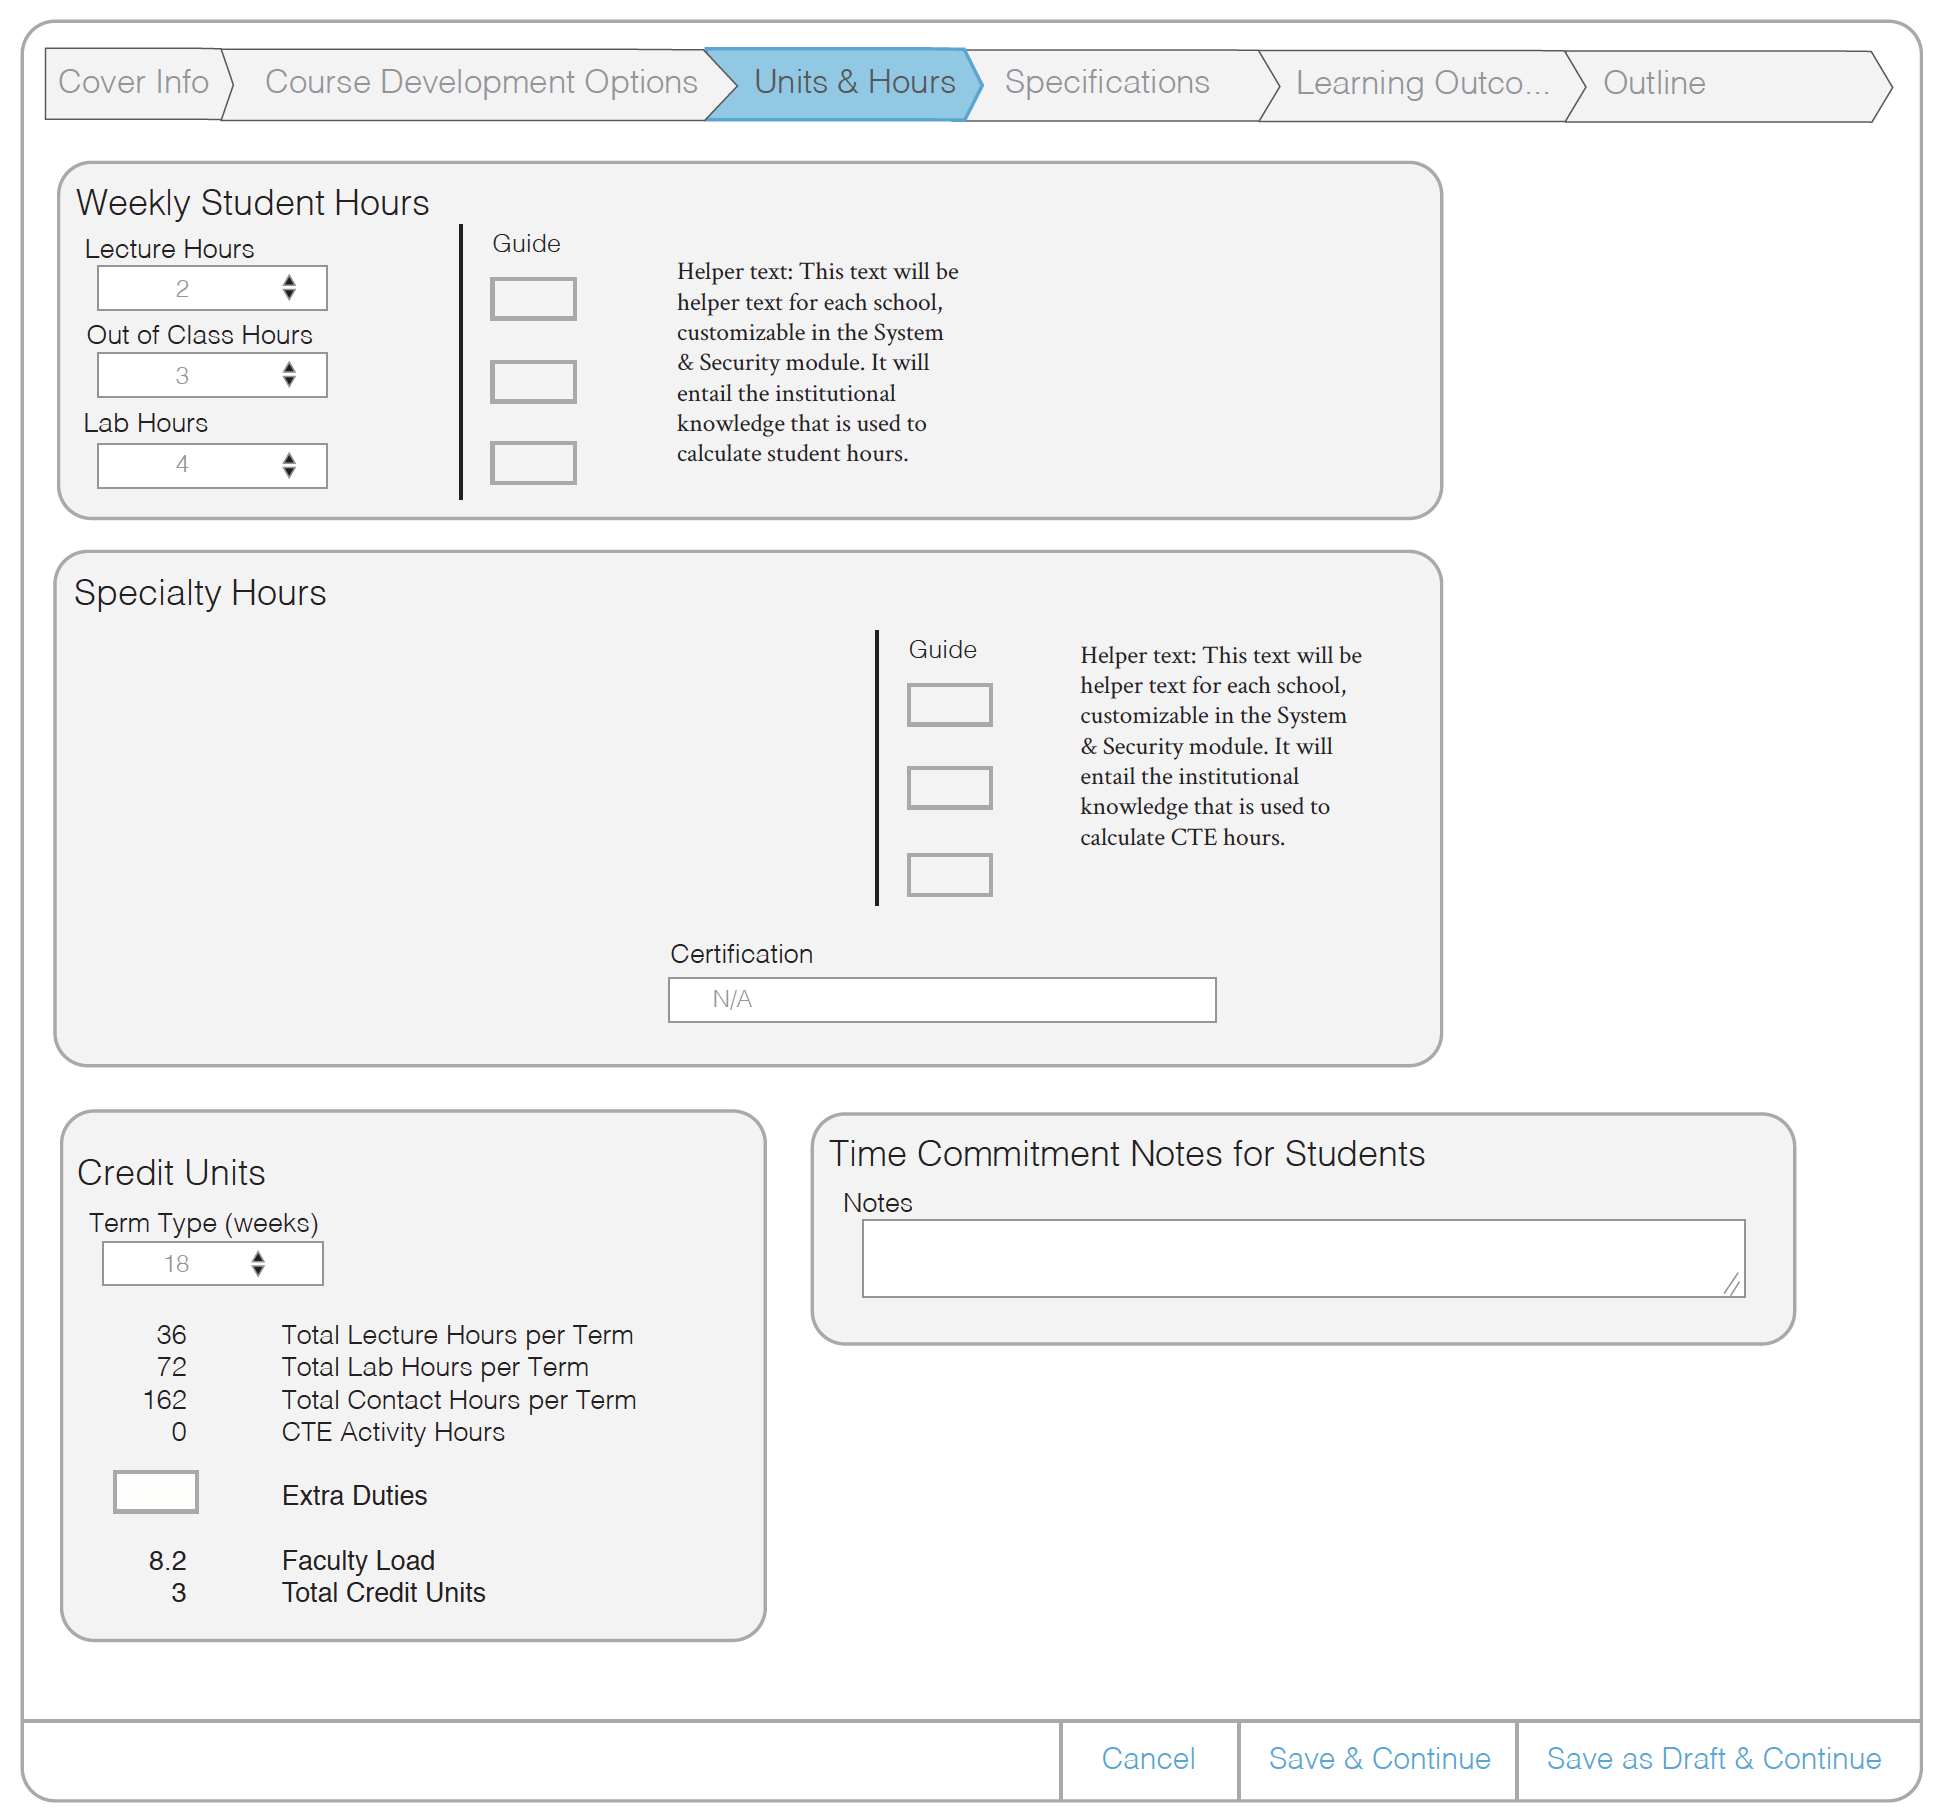
\includegraphics[scale=0.3]{Capitulos/DesarrollodelaAplicacion/Imagenes/course_units_hours}
\caption{Mockup de la pantalla de horas y unidades de evaluación de curso.}
  \label{course_units_hours}
\end{figure}

\subsection{Especificaciones de curso}
En la siguiente historia de usuario ha desarrollado un nuevo paso para el flujo de trabajo en la cual el encargado del flujo de trabajo puede agregar objetivos, información acerca de los métodos de evaluación de la materia, algunos equipos requeridos y libros que se necesitará en el curso.

Se han proporcionado de mockups (figura \ref{course_specs}) para el nuevo paso y era un criterio de aceptación de la historia de usuario seguir el mismo formato para el desarrollo de la misma.

La historia de usuario proporciona la siguiente descripción: \enquote{\textit{Como profesor encargado de curso, me gustaría ser capaz de agregar o editar especificaciones de curso como parte del flujo de trabajo de creación y/o versionamiento de mi curso para no tener que hacerlo en papel}}.

Las tareas fueron separadas y desarrolladas por los desarrolladores y eran las siguientes:
\begin{itemize}
	\item Migrar los datos para que soporte el nuevo formato de cursos.
	\item Crear y/o modificar clases de Java para el nuevo modelo de datos.
	\item Actualizar la página de plantillas de flujo de trabajo para que soporte el nuevo paso.
	\item Actualizar el visualizador de flujo de trabajo.
	\item Actualizar los servicios de guardado para creación y versionamiento de cursos y flujo de trabajos.
	\item Actualizar el servicio de aprobación de flujo de trabajo.
\end{itemize}

La historia fue terminada en una iteración con 40 horas de desarrollo cargadas en el sistema

\begin{figure}[H]
\centering
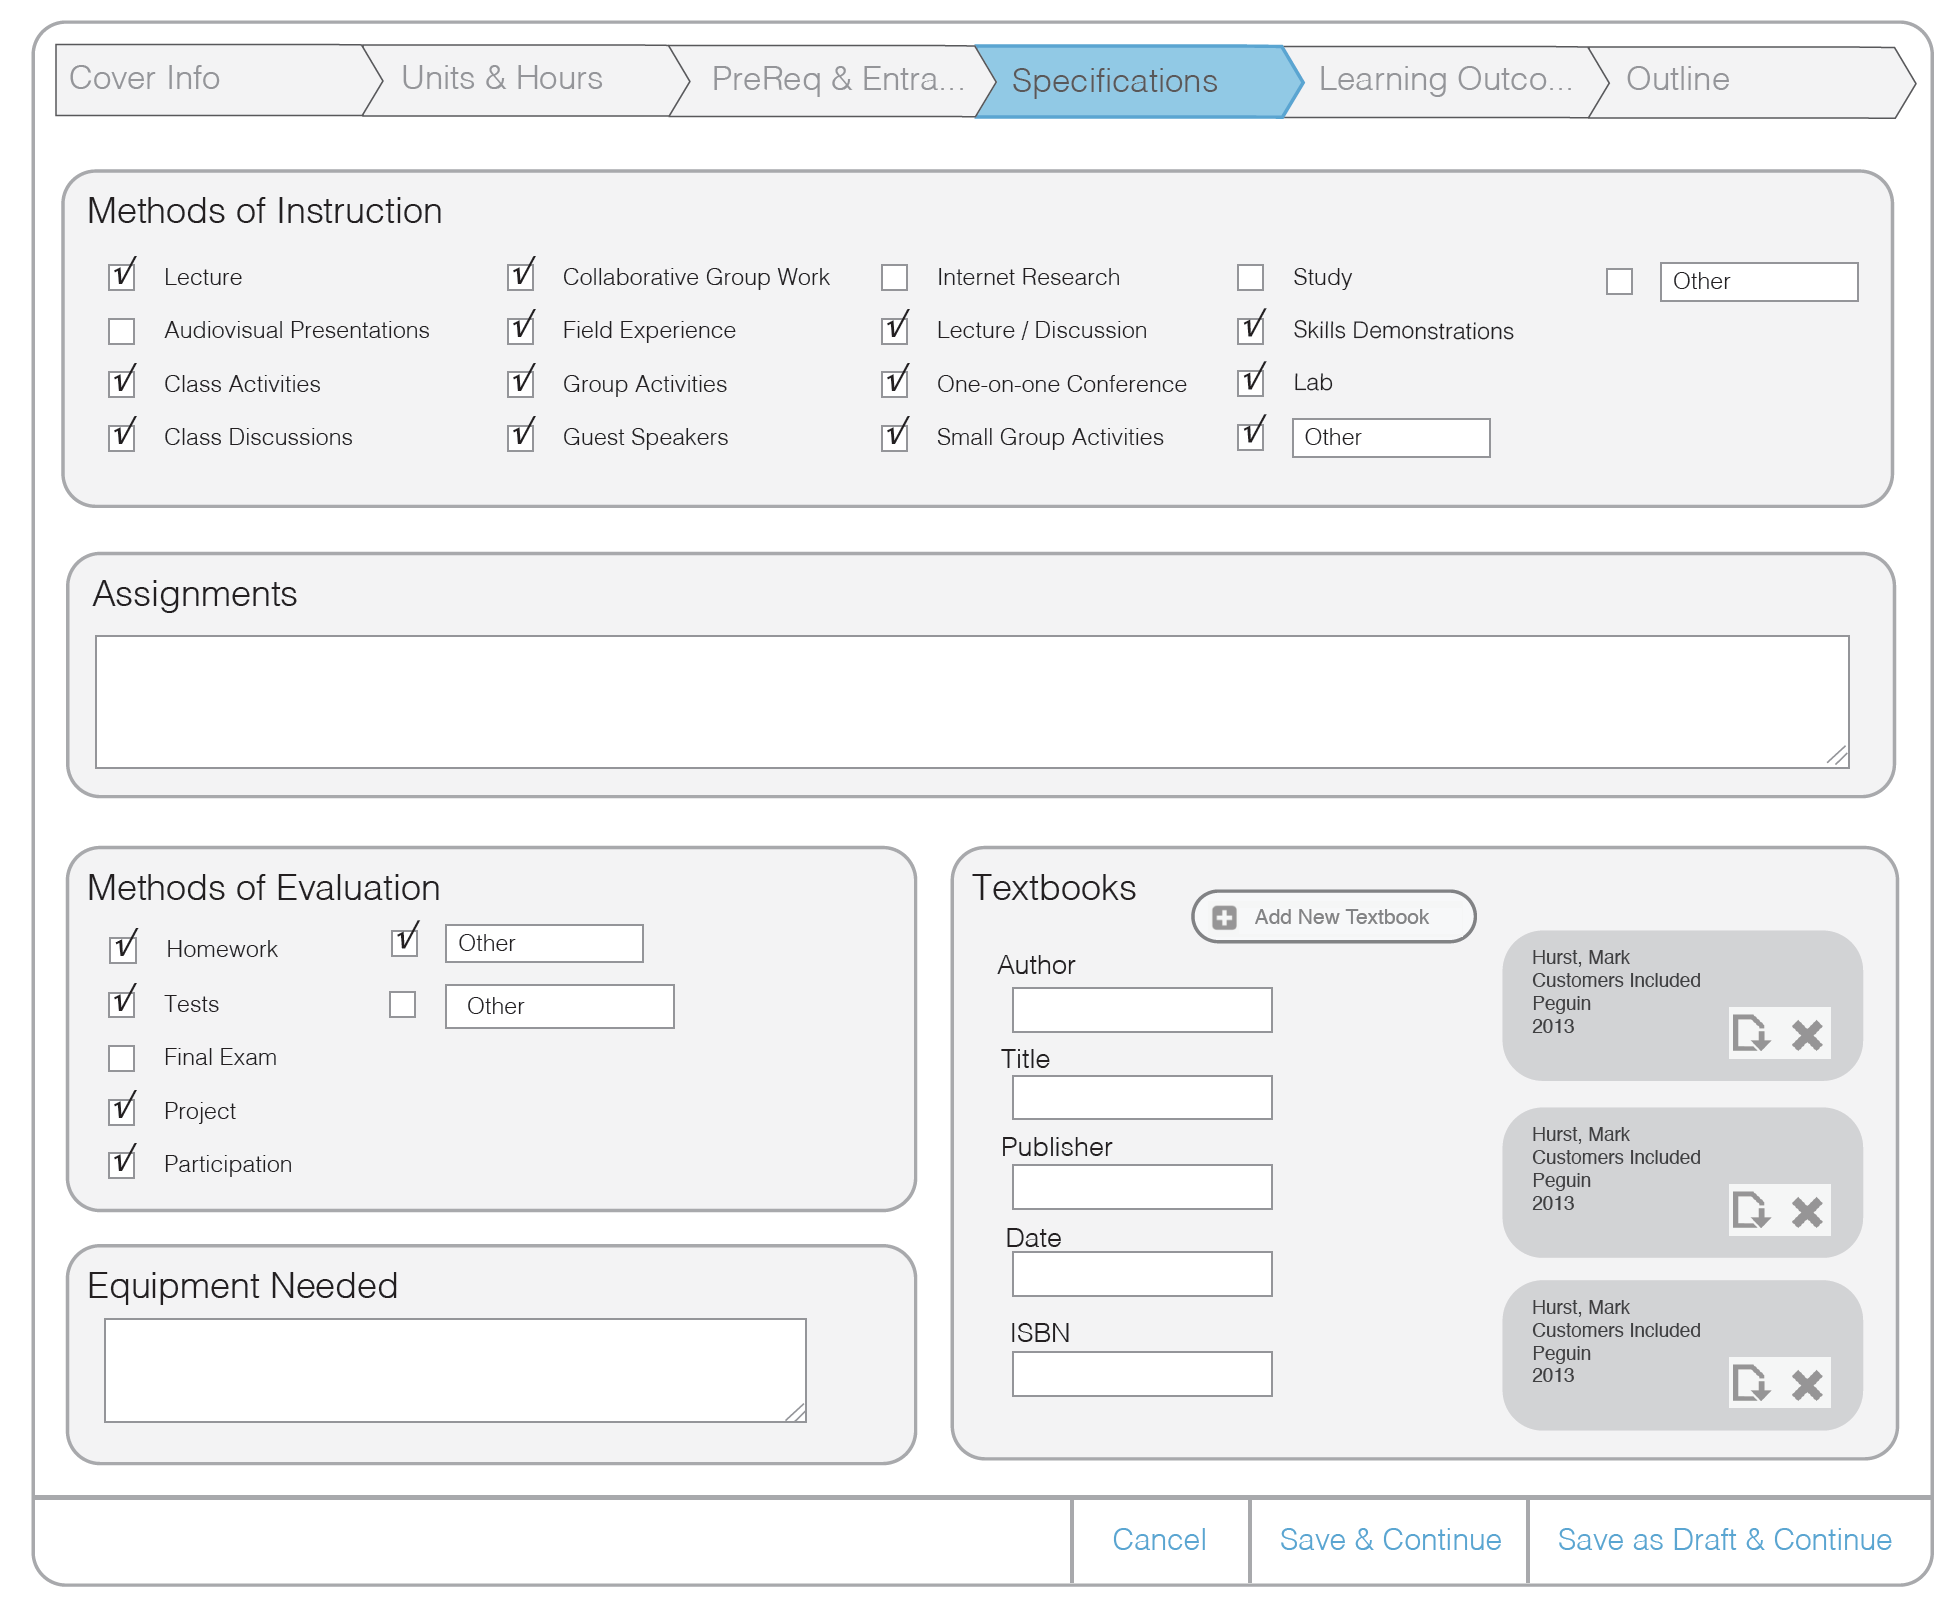
\includegraphics[scale=0.3]{Capitulos/DesarrollodelaAplicacion/Imagenes/course_specs}
\caption{Mockup de la pantalla de especificaciones de curso.}
  \label{course_specs}
\end{figure}

\subsection{Requisitos de curso}
Esta historia tiene como propósito el de adaptar el modelo de datos para que una lista de cursos como pre-requisitos, co-requisitos, anti-requisitos, y recomendaciones para su nuevo curso. Además, de ciertas capacidades que el alumno debe tener como requisito para tomar el curso.

Para entrar un poco en contexto de la historia vamos a definir cuáles son los tipos de requisitos que puede tener un curso:

\begin{itemize}
	\item \textbf{Pre-requisito:} es un tipo de requisito que impide al usuario tomar o cursar un curso sin haber aprobado antes del curso que está como pre-requisito.
	\item \textbf{Co-requisito:} es un tipo de requisito que impide al usuario tomar un curso si no cursa también el curso que tiene como co-requisito.
	\item \textbf{Anti-requisito:} es un requisito que impide al usuario tomar un curso si ya aprobó o va a tomar un curso que tiene como anti-requisito.
	\item \textbf{Recomendación:} es una recomendación por parte del sistema que materia tomar para aprovechar mejor la malla. Es opcional.
\end{itemize}

La historia de usuario tiene como descripción: \enquote{\textit{Como persona encargada de un curso, me gustaría ser capaz de introducir requisitos para cursos y ciertas competencias adquiridas en la creación o revisión de flujo de trabajo, para que podamos seguir durante su desarrollo y aprobación}} y la figura \ref{course_req} muestra mockups para la pantalla.

La historia fue dividida en partes para que los desarrolladores puedan trabajar en partes independientes durante el proceso de la misma, y eran las siguientes:
\begin{itemize}
	\item Diseñar y actualizar el modelo de datos actual.
	\item Generar y actualizar clases Java para la lógica.
	\item Actualizar la plantilla de flujo de trabajo para que soporte un nuevo paso.
	\item Actualizar el visualizador de flujo de trabajo.
	\item Actualizar los servicios de guardado y aprobación.
	\item Pruebas de funcionalidad.
\end{itemize}

La historia de usuario ha sido terminada en una iteración con 44 horas de desarrollo cargadas en el sistema.

\begin{figure}[H]
\centering
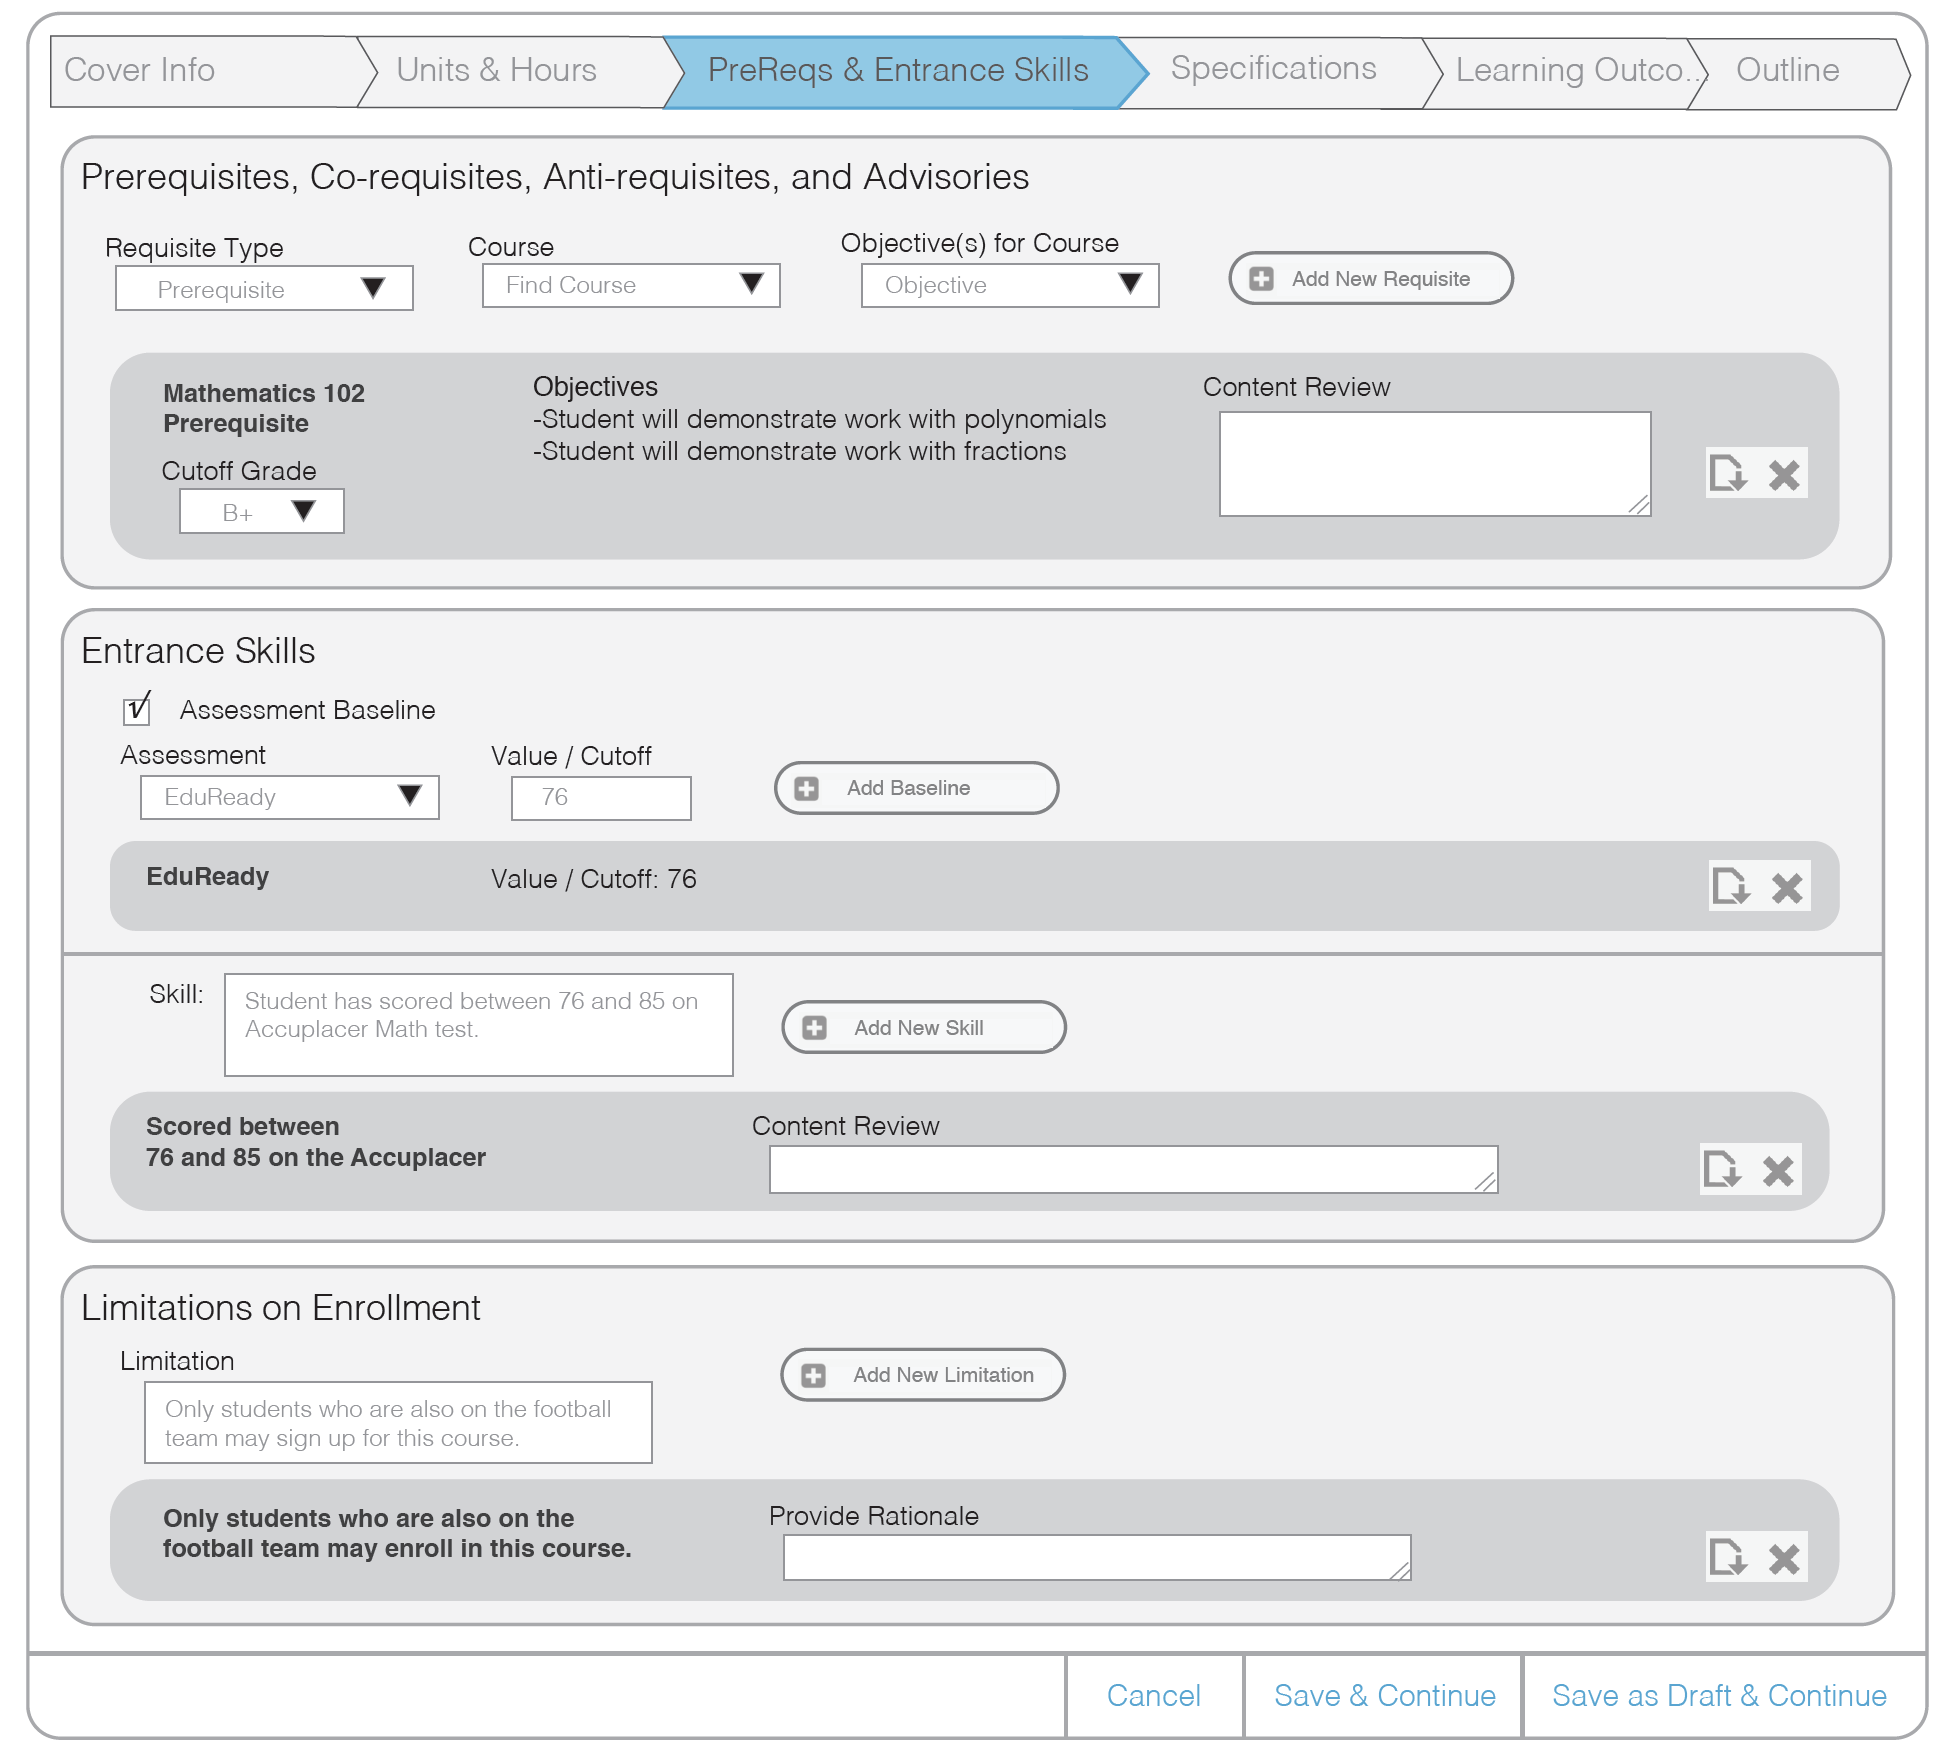
\includegraphics[scale=0.3]{Capitulos/DesarrollodelaAplicacion/Imagenes/course_req}
\caption{Mockup de la pantalla de requisitos de curso.}
  \label{course_req}
\end{figure}

\subsection{Revisar y aprobar curso}
La historia de usuario tiene como criterios de aceptación los siguientes puntos:
\begin{itemize}
	\item Las páginas para revisar los flujos de trabajos tienen una región de retroalimentación o feedback debajo de cada paso, con la opción de ocultar y mostrar para que el usuario que está revisando el flujo de trabajo en desarrollo pueda dejar comentarios al encargado del formulario del curso.
	\item La interfaz tiene elementos de estado que indican que cierta parte es nueva, aprobada, y rechazada.
	\item Los pasos tienen regiones que permiten aceptar o rechazar los campos propuestos por los desarrolladores del curso. Por lo tanto, deben tener elementos de interfaz que indiquen al usuario que puede aprobar o rechazar cada parte.
\end{itemize}
Además de los criterios de aceptación, había que volver a actualizar el buzón de entrada para que acepten los cambios que tiene la historia de usuario. Debido a que más de una persona puede revisar el flujo de trabajo y podría trancar el proceso si es que no se le notifica debidamente que hay nuevos cambios que revisar.

Algunas de las tareas descompuestas de la historia de usuario son las siguientes:
\begin{itemize}
	\item Actualizar el visualizador de flujo de trabajo para que pueda soportar la nueva característica de aprobación o rechazo de cada parte.
	\item Actualizar el buzón de entrada de Cursos.
	\item Pruebas de funcionamiento.
\end{itemize}

La historia se ha terminado en una iteración con 68 horas cargadas de desarrollo

\subsection{Competencias de curso}
Esta historia tiene como propósito de crear o versionar competencias para el curso a ser creado o versionado. 

La organización ha proporcionado mockups (figura \ref{course_learning_outcomes}) para el paso a desarrollarse y era un criterio de aceptación de parte del ticket que siga el mismo formato.

La historia de usuario tiene como descripción: \enquote{\textit{Como encargado del formulario de curso, me gustaría ser capaz de articular las competencias de mi nuevo curso, para de esa manera de tener que estar añadiendo una a una después de completar el proceso de creación de cursos con el flujo}}.

Como criterio de aceptación de la historia fue la de agregar el flujo de trabajo de competencias en el flujo de trabajo de cursos. Algunas de las tareas de la historia fueron:
\begin{itemize}
	\item Modificar la base de datos para que soporte el nuevo modelo de datos de las competencias dentro de flujo de trabajo de curso.
	\item Modificar o agregar clases de las entidades que van a ser usadas durante la historia.
	\item Actualizar la plantilla de flujo de trabajo para que soporte el nuevo paso para la creación o versionamiento de competencias.
	\item Actualizar el visualizador de flujo de trabajo para que soporte el nuevo paso de competencias.
	\item Actualizar los servicios de guardado y de versionamiento de cursos y competencias.
	\item Pruebas de nuevas funcionalidades.
\end{itemize}

La historia ha sido terminada en dos iteraciones con un total de 76 horas cargadas en el sistema.

\begin{figure}[H]
\centering
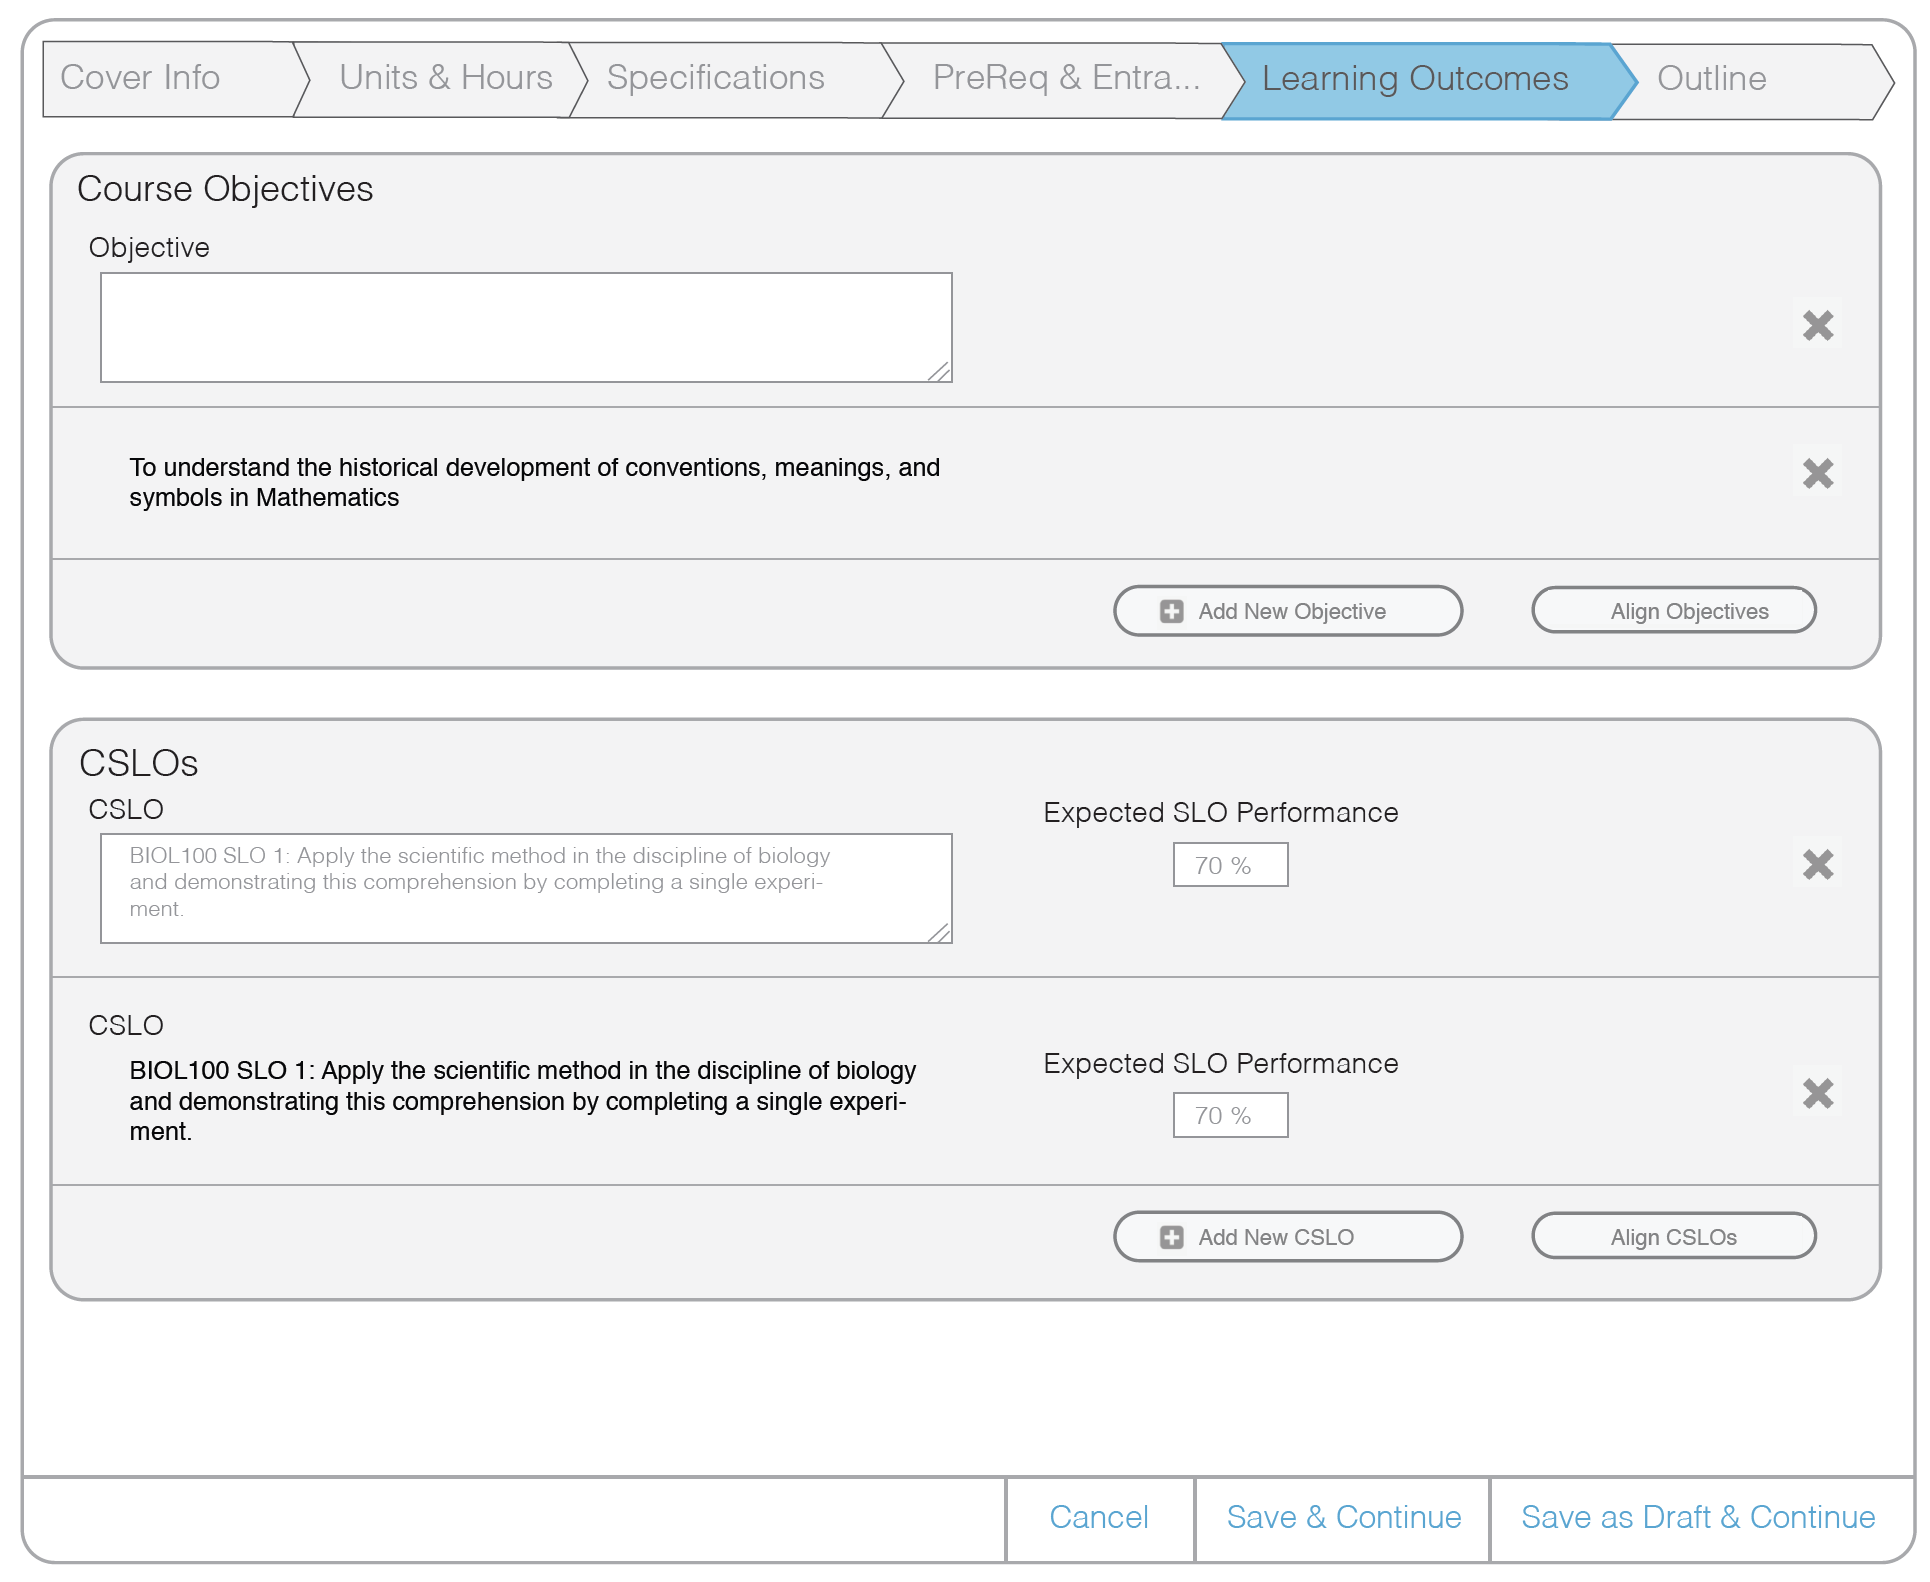
\includegraphics[scale=0.3]{Capitulos/DesarrollodelaAplicacion/Imagenes/course_learning_outcomes}
\caption{Mockup de la pantalla de competencias de curso.}
  \label{course_learning_outcomes}
\end{figure}

\subsection{Esquema de curso}
Esta historia tiene como propósito de diseñar la pantalla para un nuevo paso para el flujo de trabajo. 

La organización ha proporcionado mockups (figura \ref{course_outline}) para el paso a desarrollarse y era un criterio de aceptación de parte del ticket que siga el mismo formato.

La historia de usuario tiene como descripción: \enquote{\textit{Como encargado del formulario de curso, me gustaría ser capaz de agregar el esquema de un curso, para de esta manera dar un resumen de curso para el que esté revisando mi flujo y para que los estudiantes puedan tener una idea de se trata una vez que se curse}}.

Como criterio de aceptación de la historia fue la de agregar el flujo de trabajo de competencias en el flujo de trabajo de cursos. Algunas de las tareas de la historia fueron:
\begin{itemize}
	\item Modificar la base de datos donde se tendría que almacenar los nuevos campos de esquema ya sea para el curso y para el flujo que se desarrolla.
	\item Modificar o agregar clases de las entidades que van a ser usadas durante la historia.
	\item Actualizar la plantilla de flujo de trabajo para que soporte el nuevo paso de esquema de cursos.
	\item Actualizar el visualizador de flujo de trabajo para que soporte el nuevo paso de competencias.
	\item Actualizar los servicios de guardado y de revisión para que soporte nuevo paso.
\end{itemize}

La historia ha sido terminada en dos iteraciones con un total de 48 horas cargadas en el sistema.

\begin{figure}[H]
\centering
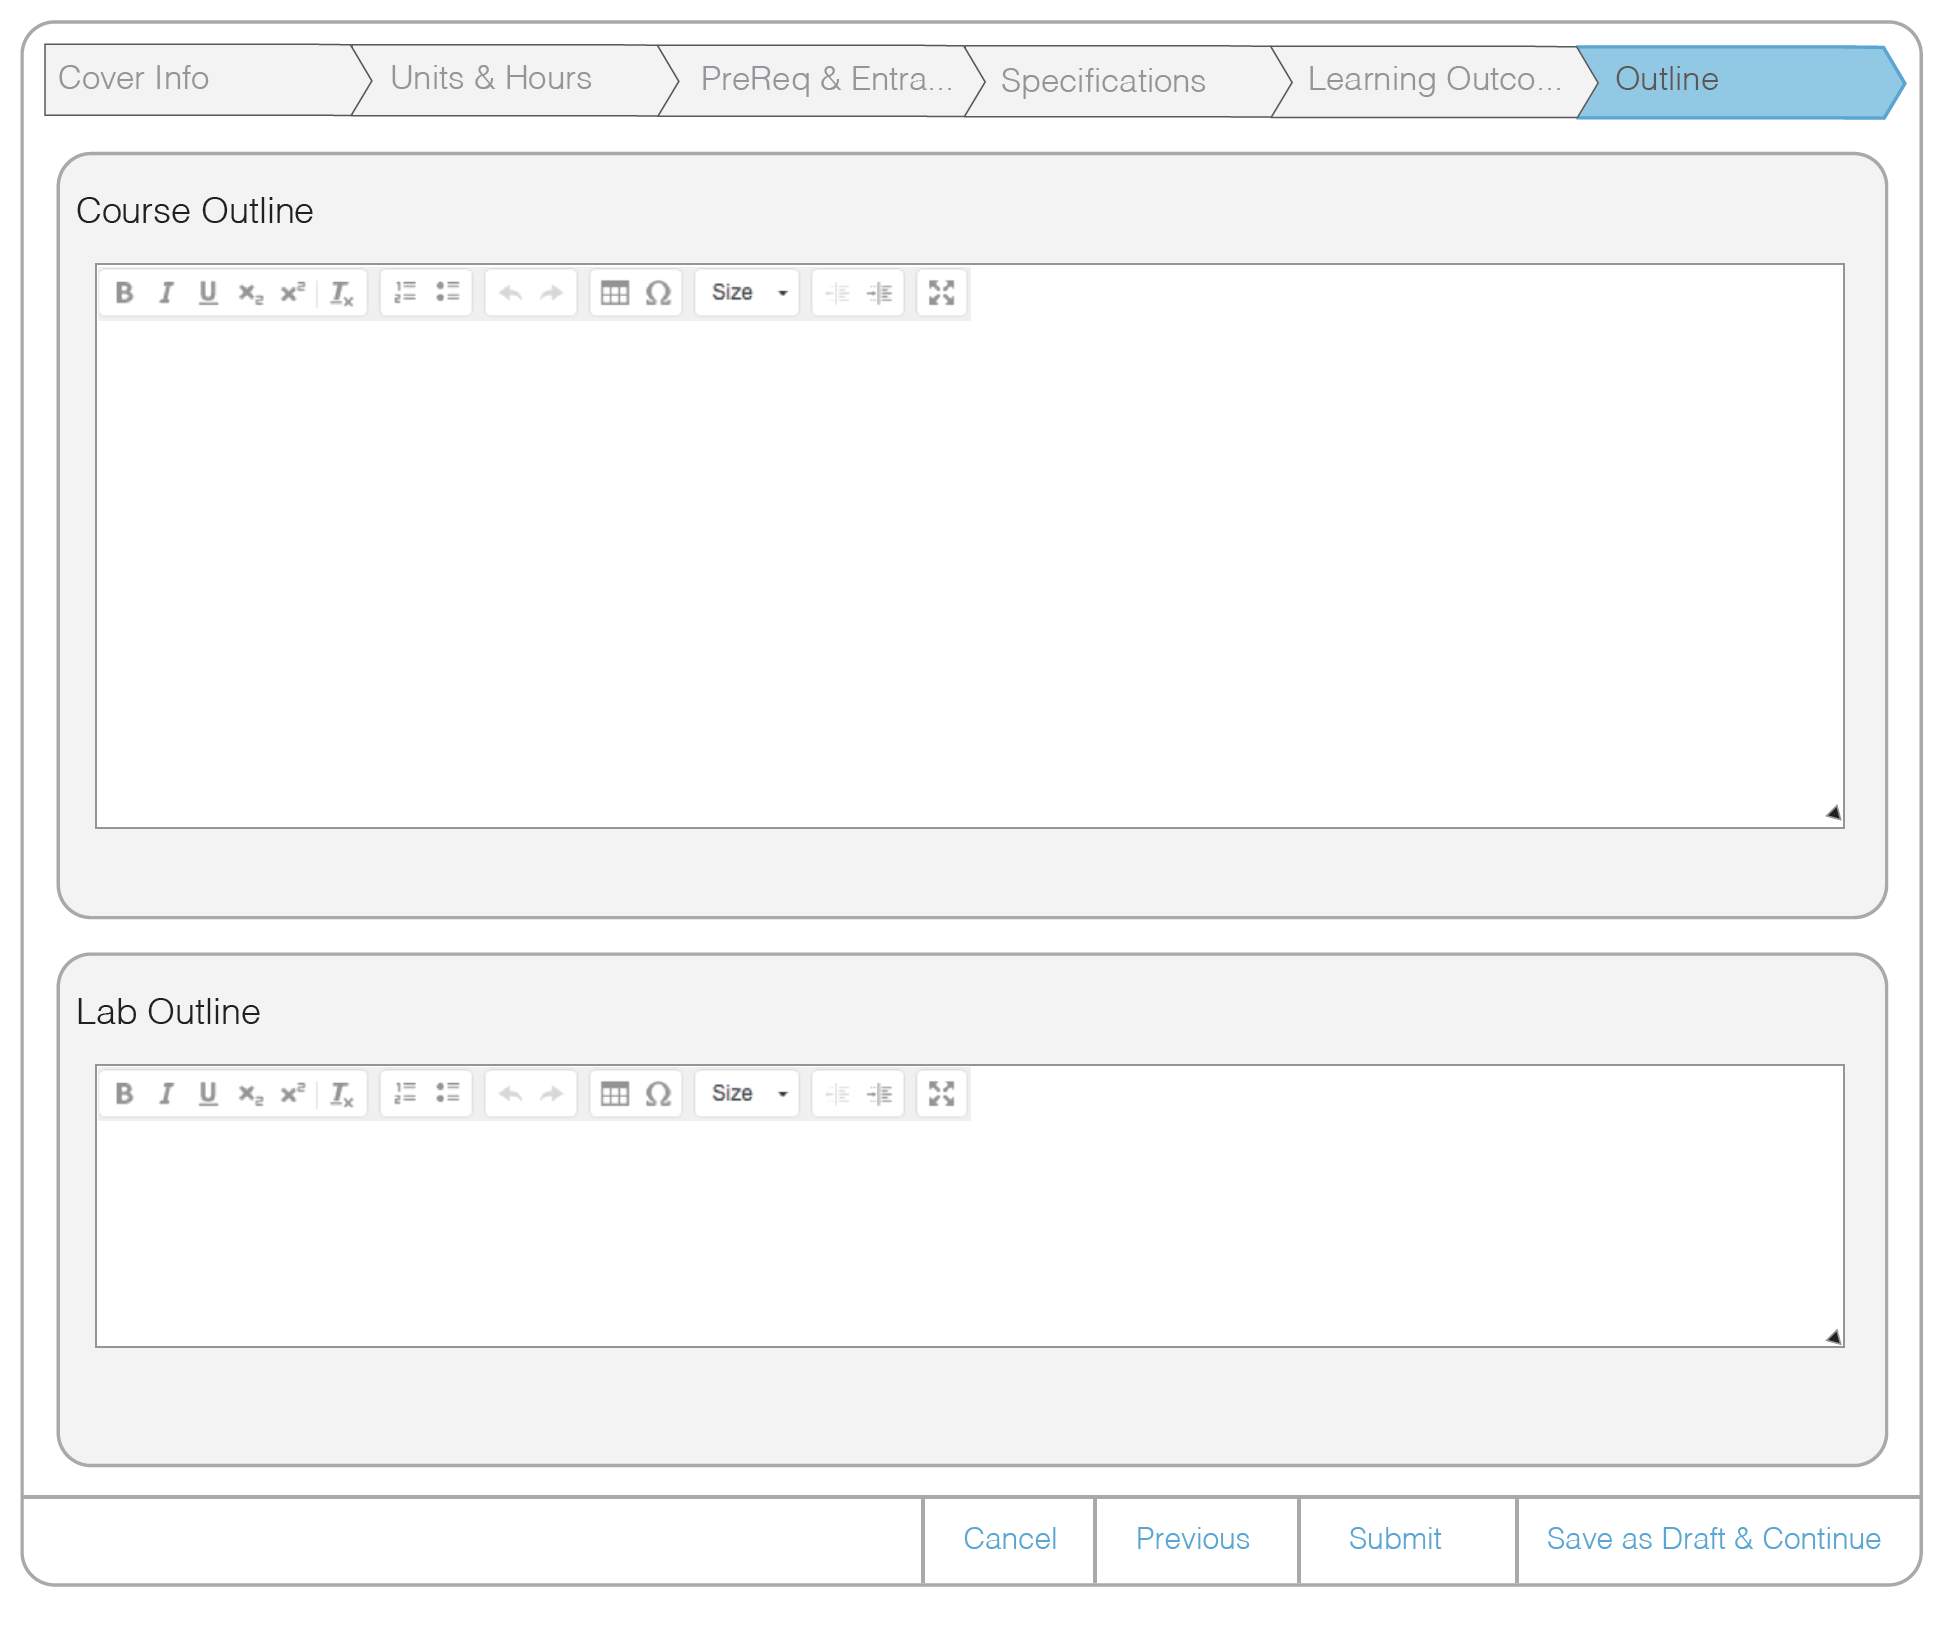
\includegraphics[scale=0.3]{Capitulos/DesarrollodelaAplicacion/Imagenes/course_outline}
\caption{Mockup de la pantalla de esquema de curso.}
  \label{course_outline}
\end{figure}

\subsection{Códigos de clasificación de curso}
Esta historia tiene como propósito la de asignar códigos de clasificación a los cursos.

Para entrar en contexto, habría que definir primero que es TOP\footnote{de sus siglas en inglés, Taxonomy Of Programs, que significa en español taxonomía de programas.}.

TOP es un sistema numérico de códigos usados a nivel de Estado para recolectar y reportar información en cursos y programas, en diferentes instituciones educativas \citep{brice_w_harris_program_2013} por todo el Estado. 

Ha sido diseñado para agregar información acerca de los programas. Sin embargo, un código TOP debe ser asignado a cada curso del sistema. 

Aunque no contiene tantas opciones específicas como lo haría un sistema diseñado para cursos, a cada curso se le debe dar el código que se aproxima a describir el contenido del curso.

Algunos usos a los códigos:
\begin{itemize}
	\item En el inventario de programas aprobados y rechazados, para tener información que tipos de cursos y programas son ofrecidas por el estado.
	\item En bases de datos de administración de información, para recolectar y reportar información en logros estudiantiles (licenciaturas y certificados) en ciertos programas.
	\item En contabilidad vocacional estudiantil, para reportes de compleción de programas y cursos de ciertos programas vocacionales.
\end{itemize}

La historia de usuario tiene como descripción: \enquote{\textit{Como miembro del comité curricular, me gustaría ser capaz de asignar a mis cursos de códigos de clasificación como parte de la aprobación de mis flujo de trabajos para asegurar que estén correctos, como esto es motivo de rechazo en la oficina del canciller del Estado}}.

Algunas de las tareas fueron las siguientes:
\begin{itemize}
	\item Diseño del nuevo modelo, donde se debían generar tablas para cada nueva entidad del modelo de datos ajustado para las taxonomías de programas. Además, cargar todos los datos de códigos de cursos existentes para el estado de California.
	\item Creación de clases Java.
	\item Diseño e implementación páginas CRUD para disciplina, sub-disciplina, y campo.
	\item Diseño e implementación de la nueva página de asignación de códigos de clasificación para los cursos en proceso de diseño.
	\item Hacer servicios para cada una de las nuevas páginas.
	\item Pruebas de funcionalidad.
\end{itemize}

La historia de usuario ha sido terminada en una iteración con 80 horas cargadas en el sistema.
\section{Flujo de trabajo para el versionamiento de programas de estudio}
\begin{table}[H]
\centering
\resizebox{\columnwidth}{!}{%
\begin{tabular}{@{}lllll@{}}
\toprule
Historias de usuario               & HE  & HC  & PH & Sprints \\ \midrule
Información básica del programa    & 54  & 56  & 8  & 1       \\
Competencias de carrera o programa & 48  & 68  & 5  & 1       \\
Bloques de curso                   & 58  & 60  & 5  & 1       \\
Visualizar cambios en los campos   & 180 & 210 & 13 & 4       \\ \bottomrule
\end{tabular}
}
\caption{Historias de usuario para flujo de trabajo para el versionamiento de programas de estudio}
\label{epic:8}
\end{table}

\subsection{Información básica del programa}
La historia de usuario tiene como descripción lo siguiente \enquote{\textit{Como coordinador del departamento o encargado del AMS, me gustaría ser capaz de agregar o revisar programas en el módulo de gestión curricular, para que de esta forma pueda manejar mejor mis registros de la institución en el sistema}}. Y los criterios de aceptación consistían en el desarrollo de la pantalla que se puede apreciar en la figura \ref{program_cover_info}.

Algunas de las tareas identificadas en la planificación de las iteraciones eran los siguientes:
\begin{itemize}
	\item Adaptar la base de datos para soportar los nuevos campos a ser guardados por el flujo de trabajo.
	\item Luego de hacer los cambios en la base de datos, actualizar o agregar nuevas clases de Java para su posterior uso.
	\item Desarrollar la página de información básica del programa.
	\item Actualizar la plantilla de flujos de trabajo institucional para que soporte la creación y revisión de programas.
	\item Diseñar servicios para guardar los registros de la nueva página.
	\item Diseñar servicios de aprobación de flujo de trabajo de programas.
\end{itemize}

La historia fue finalizada en una iteración con una cantidad de 56 horas cargadas en el sistema.

\begin{figure}[H]
\centering
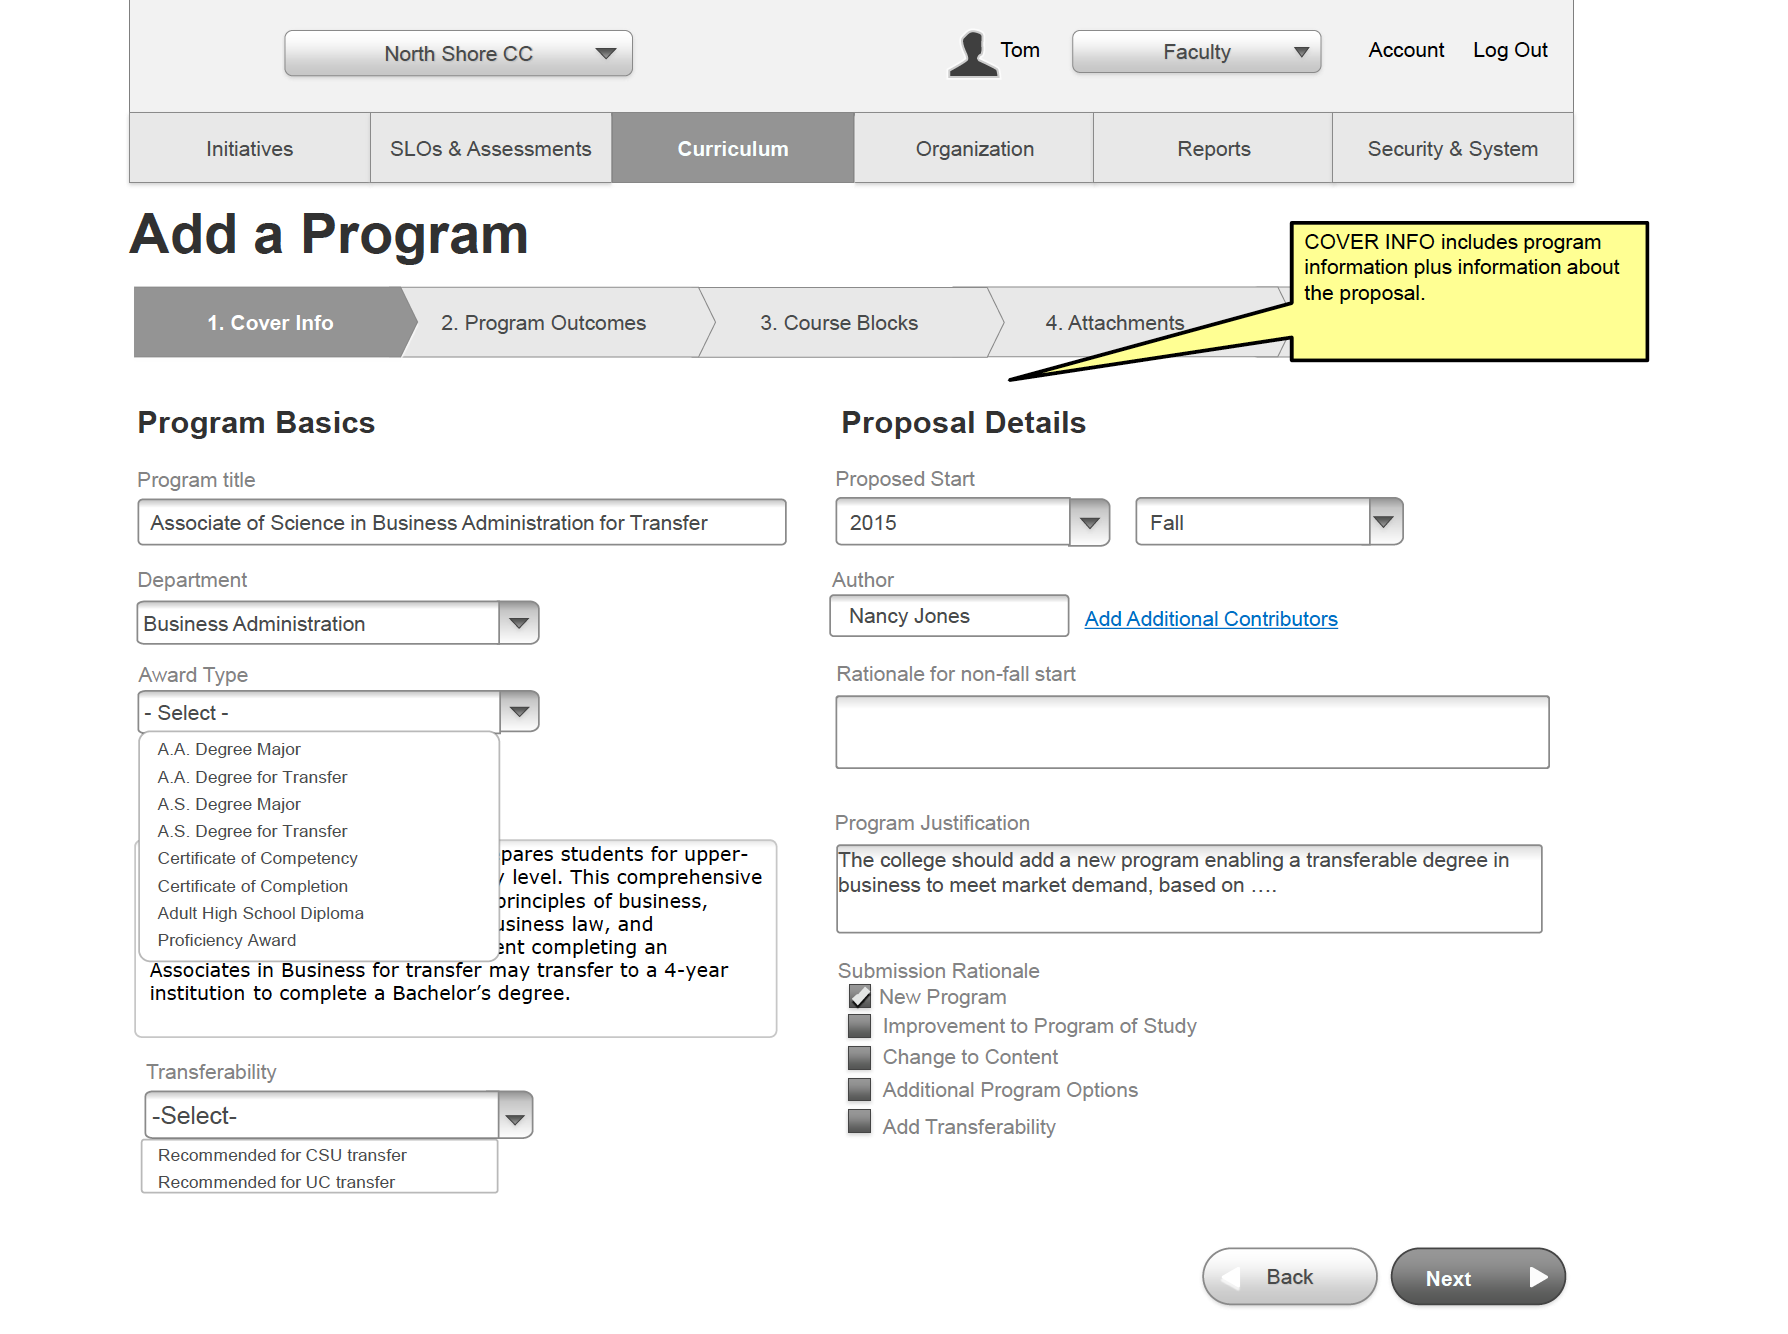
\includegraphics[width=125mm,scale=1]{Capitulos/DesarrollodelaAplicacion/Imagenes/program_cover_info}
\caption{Mockup de la pantalla de información básica del programa.}
  \label{program_cover_info}
\end{figure}

\subsection{Competencias de carrera o programa}
La historia de usuario tiene como descripción lo siguiente \enquote{\textit{Como coordinador, me gustaría ser capaz de administrar las competencias asociadas a mi programas durante el flujo de creación y revisión del mismo, para que pueda hacer una revisión comprensiva de los programas que tiene el AMS}}. Y los criterios de aceptación consistían en el desarrollo de la pantalla que se puede apreciar en la figura \ref{program_learning_outcomes}.

Algunas de las tareas identificadas en la planificación de las iteraciones eran los siguientes:
\begin{itemize}
	\item Adaptar la base de datos para soportar los nuevos campos a ser guardados por el flujo de trabajo.
	\item Luego de hacer los cambios en la base de datos, actualizar o agregar nuevas clases de Java para su posterior uso.
	\item Desarrollar la página de información básica del programa.
	\item Actualizar los servicios de guardado de campos para el flujo de trabajo.
	\item Actualizar los servicios de aprobación de flujo de trabajo de programas.
\end{itemize}

La historia fue finalizada en una iteración con una cantidad de 68 horas cargadas en el sistema.

\begin{figure}[H]
\centering
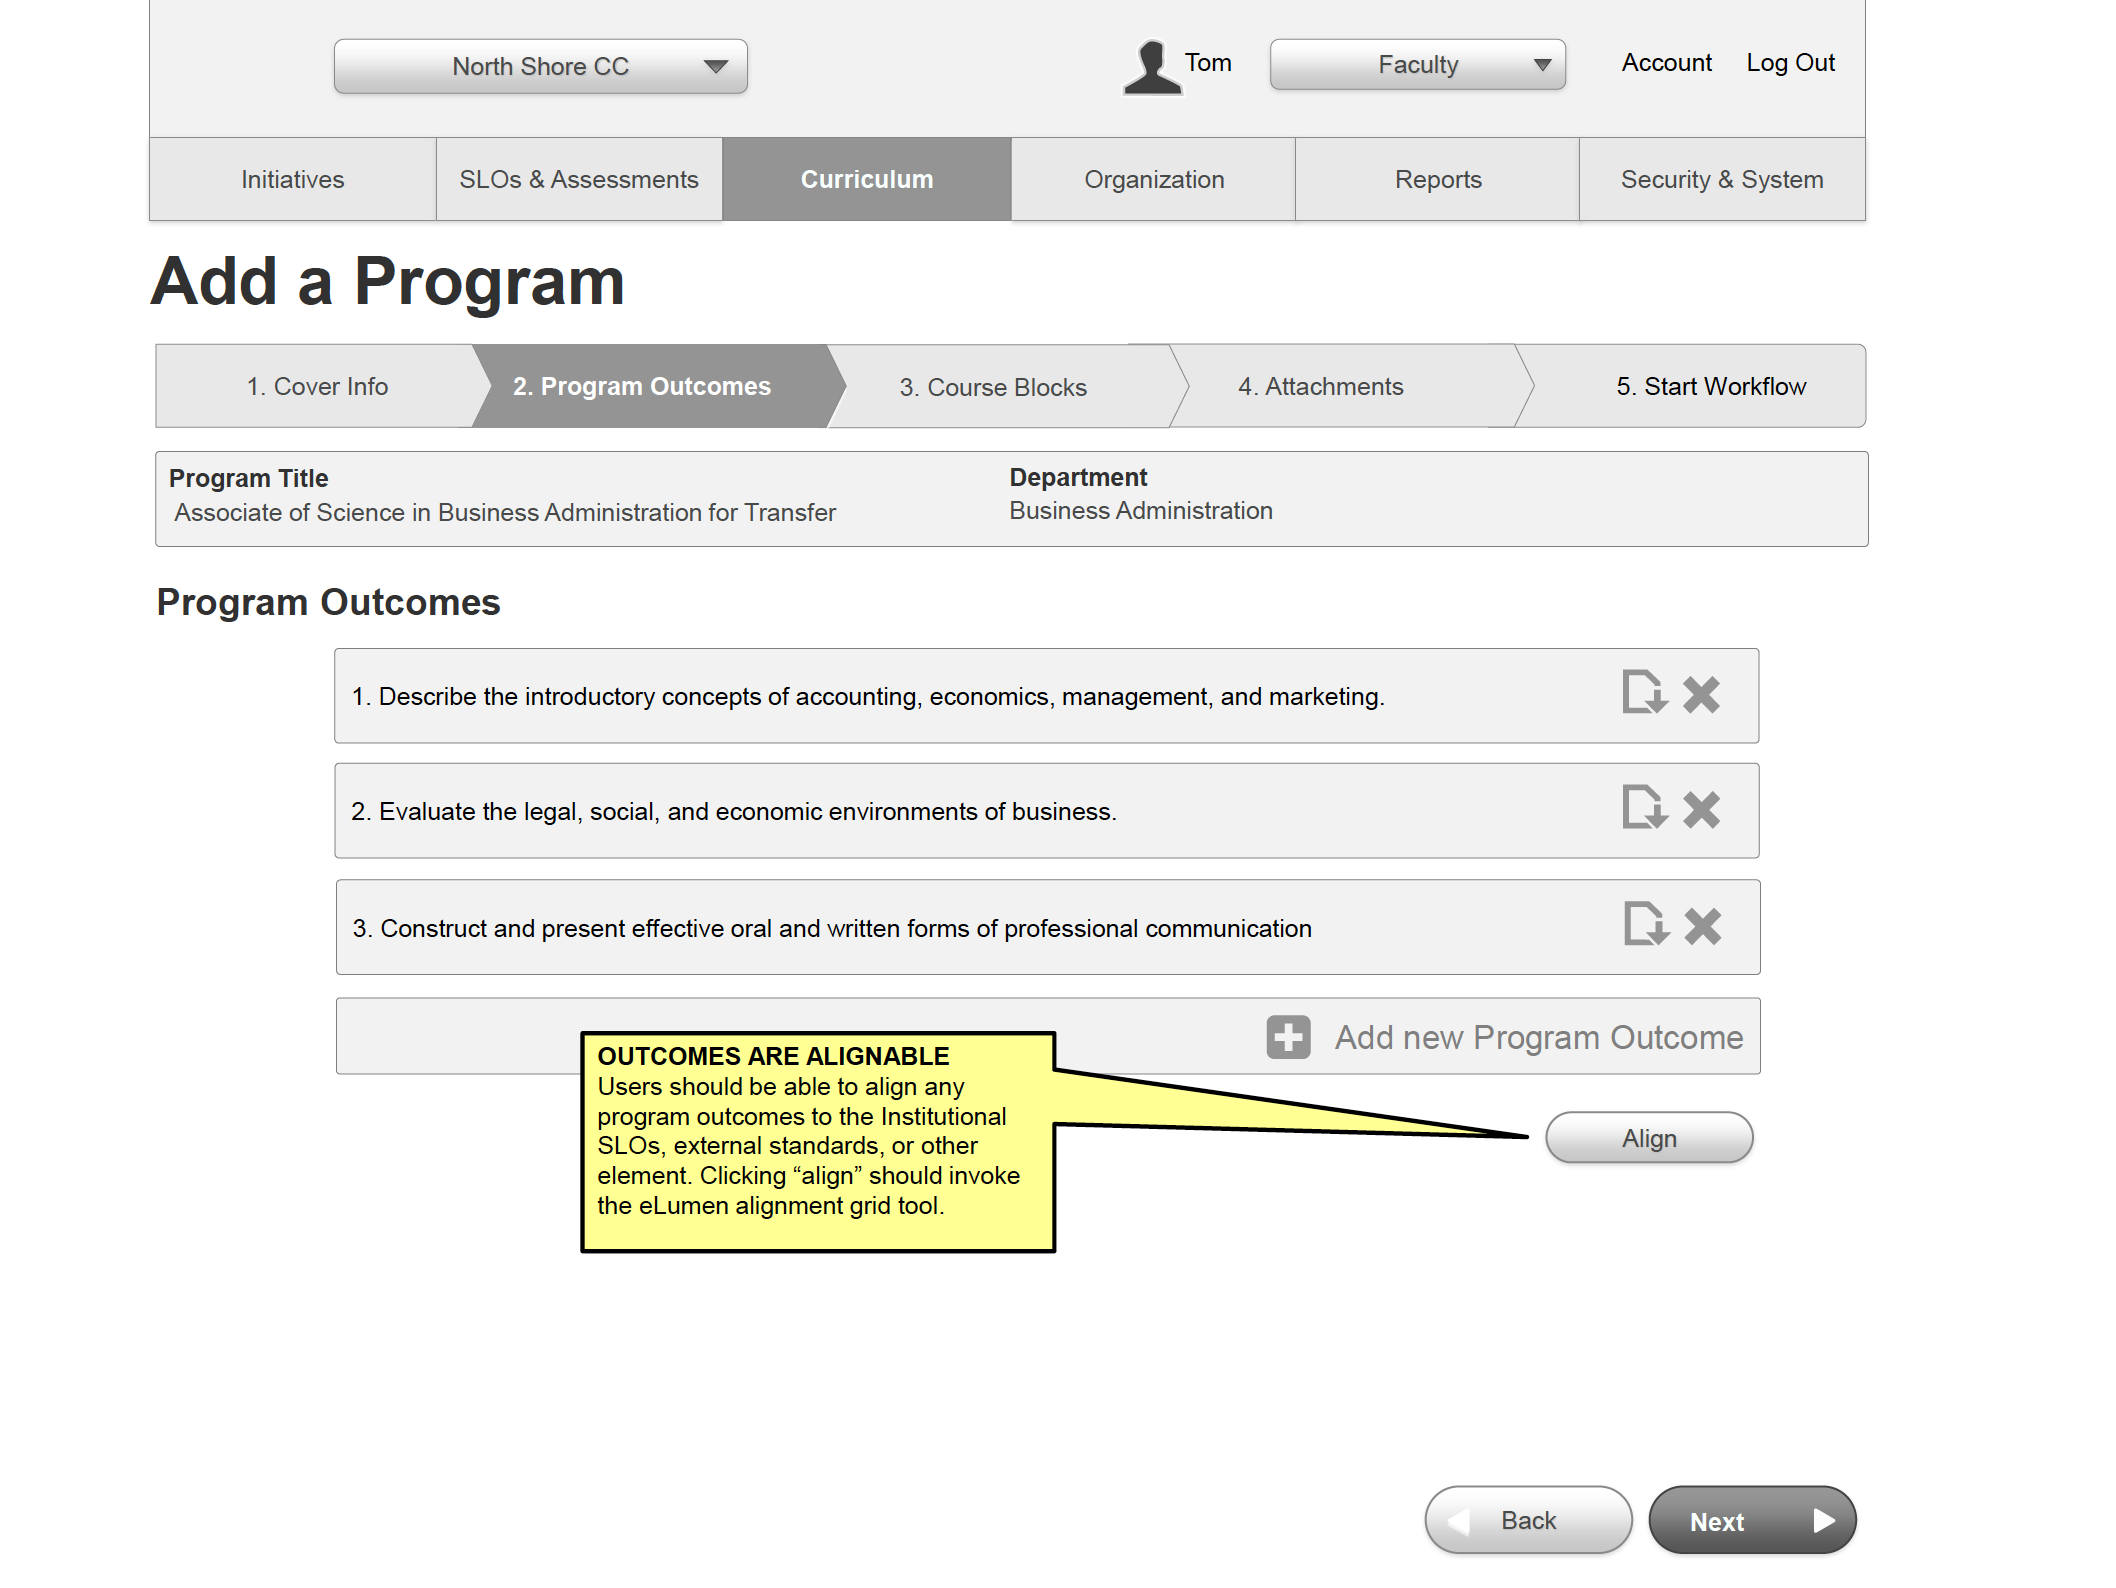
\includegraphics[width=125mm,scale=1]{Capitulos/DesarrollodelaAplicacion/Imagenes/program_learning_outcomes}
\caption{Mockup de la pantalla de competencias del programa.}
  \label{program_learning_outcomes}
\end{figure}

\subsection{Bloques de cursos}
La historia de usuario tiene como descripción lo siguiente \enquote{\textit{Como coordinador de departamento, me gustaría ser capaz de diseñar bloques de cursos para mis programas, para que de esta manera pueda diseñar la malla para mis programas de estudio}}. Y los criterios de aceptación consistían en el desarrollo de la pantalla que se puede apreciar en la figura \ref{program_course_blocks}.

Algunas de las tareas identificadas en la planificación de las iteraciones eran los siguientes:
\begin{itemize}
	\item Diseño e implementación del modelo de datos.
	\item Diseño e implementación de clases Java.
	\item Desarrollar la página de paso para creación de bloques de cursos en los diferentes flujos de trabajo.
	\item Desarrollar servicios de guardado y aprobación de la funcionalidad.
	\item Actualizar la plantilla de flujos de trabajo.
\end{itemize}

La historia fue finalizada en una iteración con una cantidad de 60 horas cargadas en el sistema.

\begin{figure}[H]
\centering
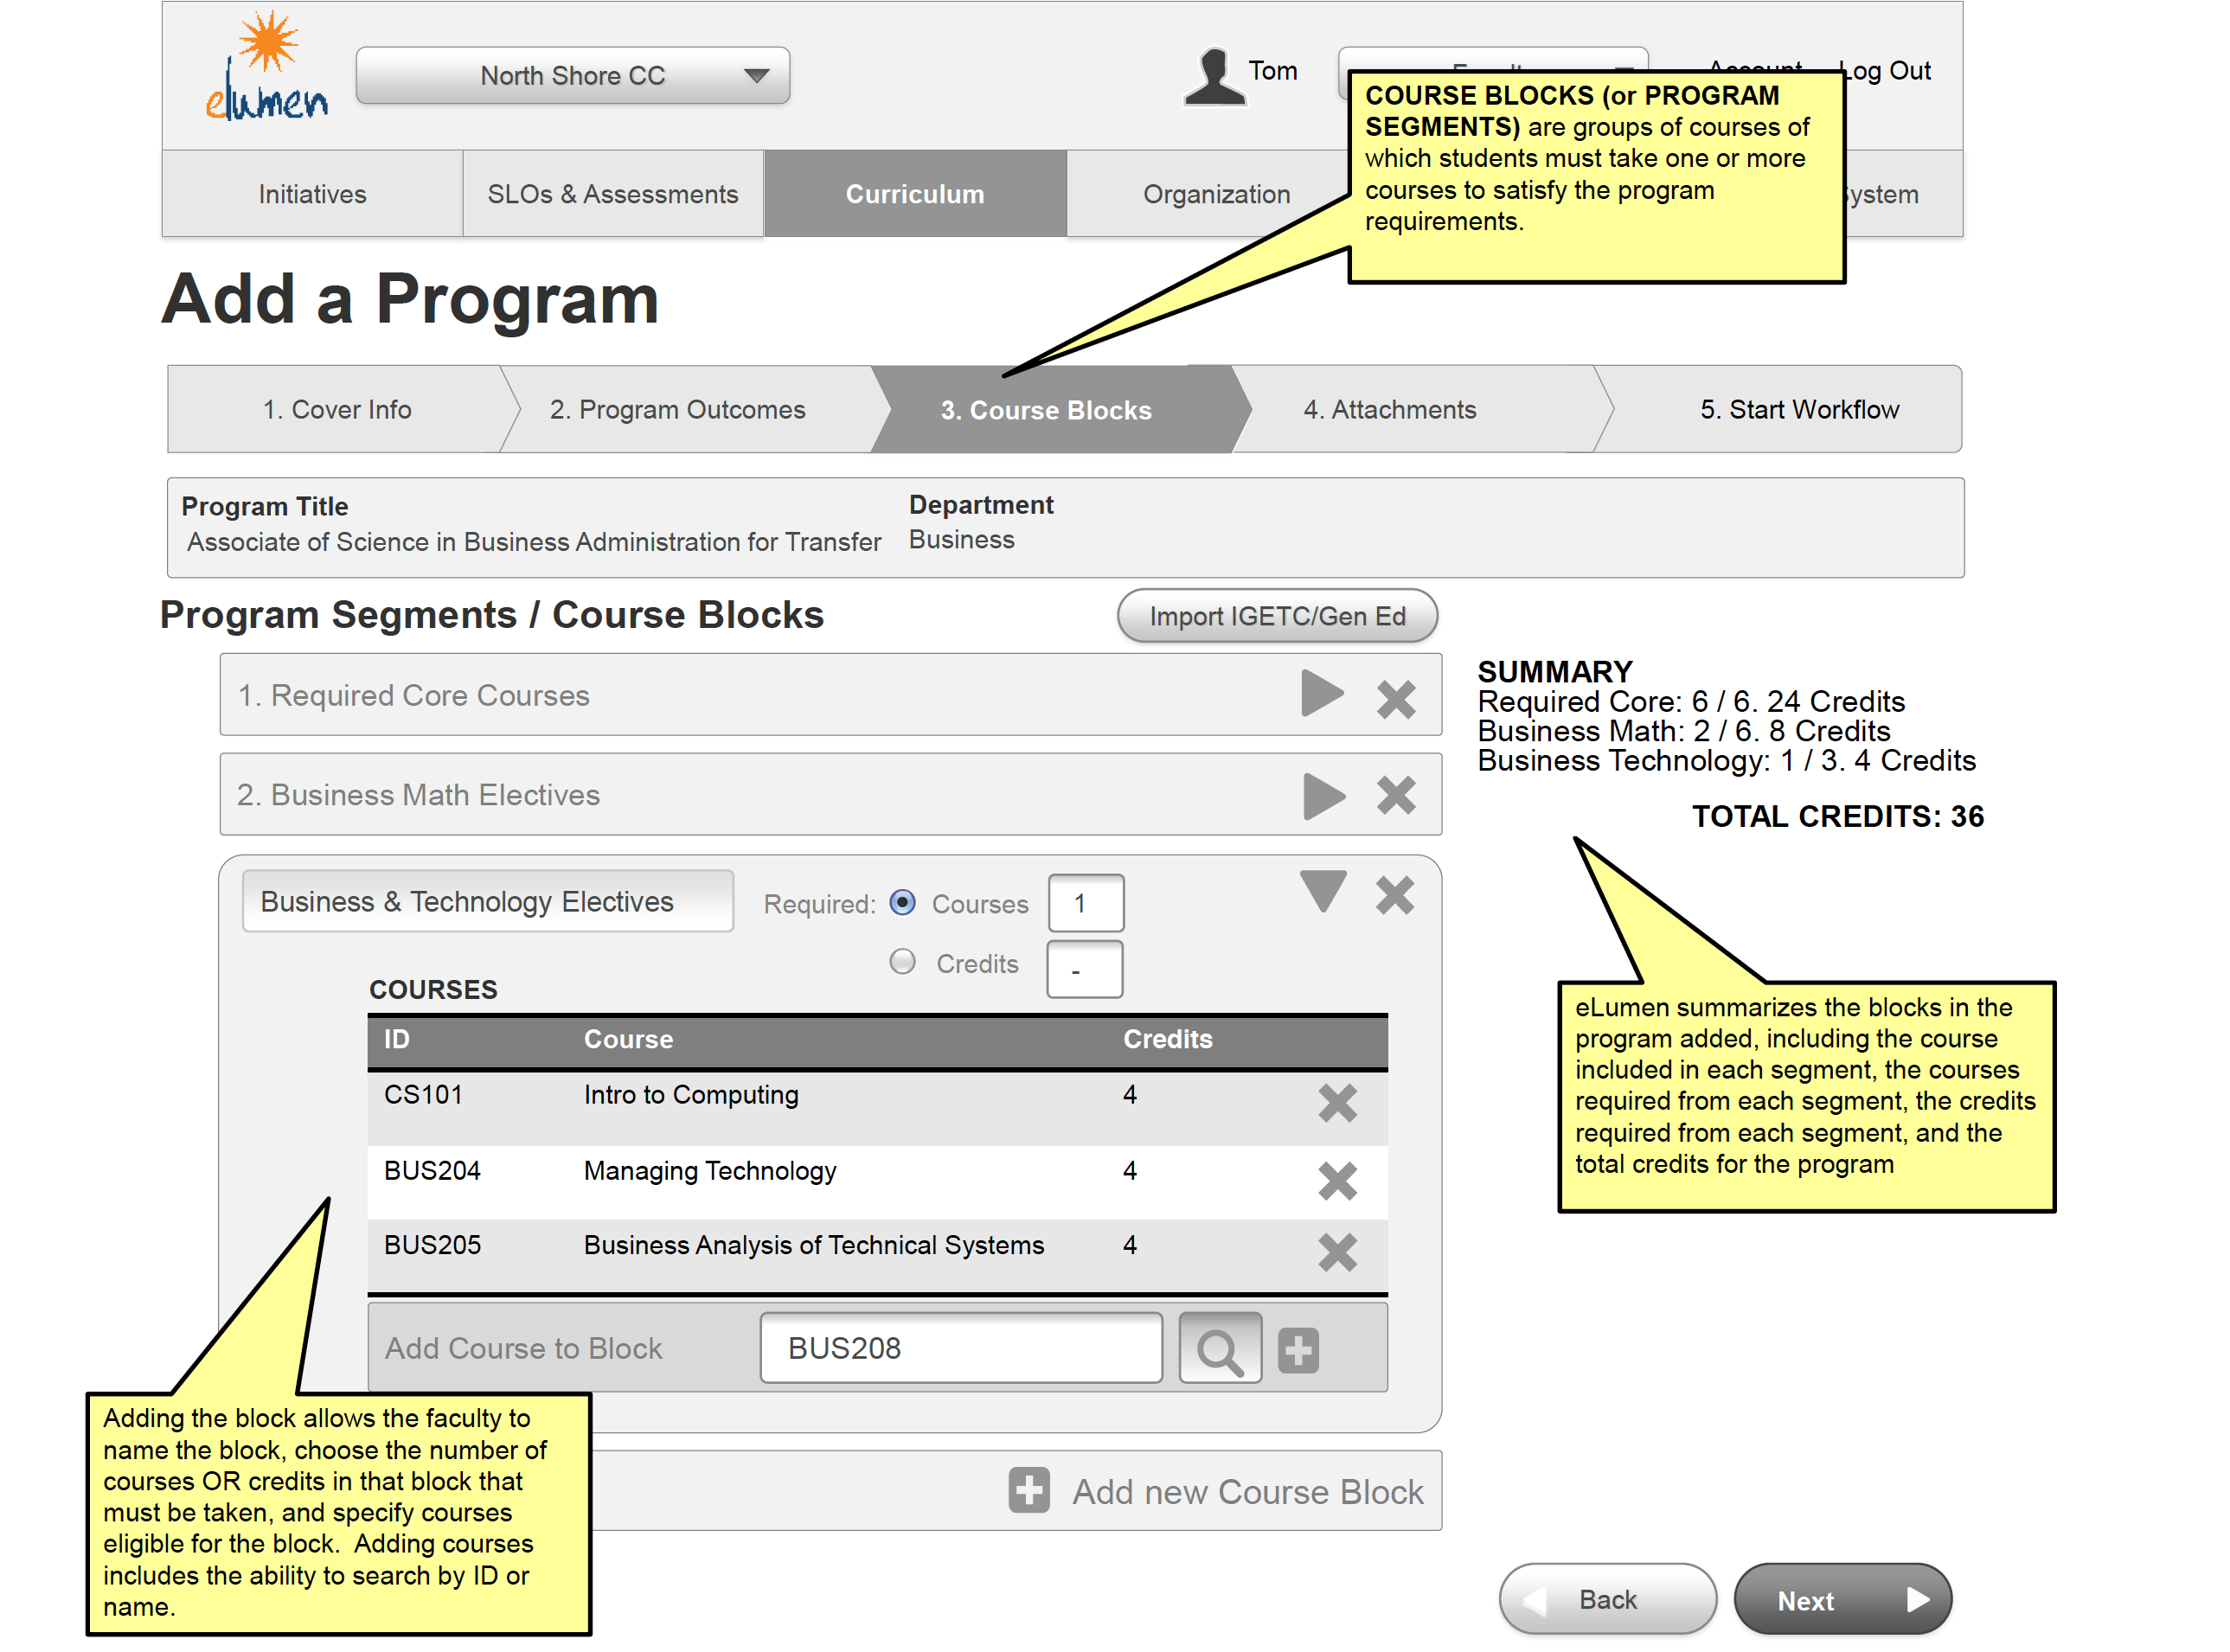
\includegraphics[width=125mm,scale=1]{Capitulos/DesarrollodelaAplicacion/Imagenes/program_course_blocks}
\caption{Mockup de la pantalla de bloques de cursos de programa.}
  \label{program_course_blocks}
\end{figure}

\subsection{Visualizar cambios en los campos}
La historia de usuario tiene como descripción lo siguiente \enquote{\textit{Como coordinador de departamento, me gustaría ser capaz de diseñar bloques de cursos para mis programas, para que de esta manera pueda diseñar la malla para mis programas de estudio}}. Y los criterios de aceptación consistían en el desarrollo de la pantalla que se puede apreciar en la figura \ref{visualize_changes}.

Como criterios de aceptación se encuentran los siguientes:
\begin{itemize}
	\item Los campos borrados se deben marcar en rojo.
	\item Los nuevos campos se deben marcar en verde.
	\item Se debe visualizar el estado anterior y el nuevo con una forma de identificar con el usuario que hizo la modificación.
	\item Limitado para los cambios del programa.
	\item Diseño de interfaz aprobada por el equipo de validación.
	\item Las diferencias limitadas a dos versiones.
\end{itemize}

Algunas de las tareas identificadas en la planificación de las iteraciones eran los siguientes:
\begin{itemize}
	\item Diseño e implementación del modelo de datos.
	\item Diseño e implementación de clases Java.
	\item Desarrollar la página de paso para creación de bloques de cursos en los diferentes flujos de trabajo.
	\item Desarrollar servicios de guardado y aprobación de la funcionalidad.
	\item Actualizar la plantilla de flujos de trabajo.
\end{itemize}

La historia fue finalizada en una iteración con una cantidad de 60 horas cargadas en el sistema.

\begin{figure}[H]
\centering
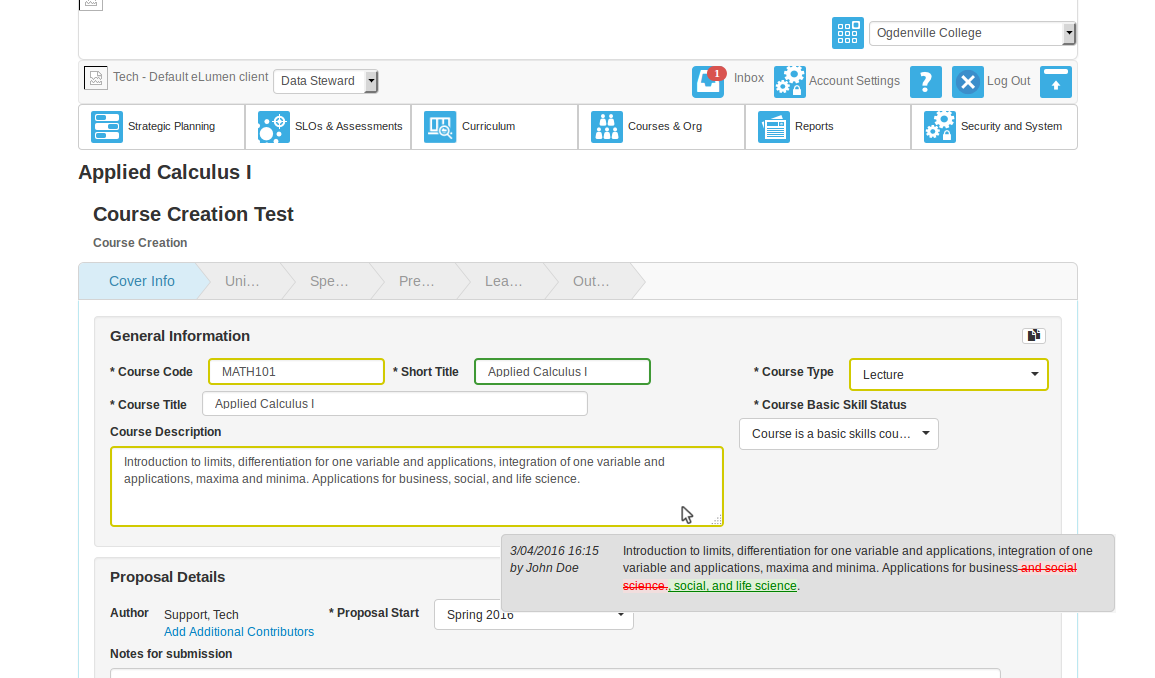
\includegraphics[width=125mm,scale=1]{Capitulos/DesarrollodelaAplicacion/Imagenes/visualize_changes}
\caption{Mockup de la pantalla de la funcionalidad de visualización de cambios.}
  \label{visualize_changes}
\end{figure}

\section{Soporte de etapas en los flujos de trabajo}
\begin{table}[H]
\centering
\resizebox{\columnwidth}{!}{%
\begin{tabular}{@{}lllll@{}}
\toprule
Historias de usuario                                             & HE  & HC  & PH & Sprints \\ \midrule
Roles de creación y edición para las partes de flujos de trabajo & 102 & 112 & 13 & 1       \\
Diseño e implementación de etapas                                & 288 & 505 & 21 & 3       \\
Mejora en comportamientos para las etapas por roles              & 84  & 108 & 8  & 2       \\
Composición de etapas y partes                                   & 216 & 391 & 13 & 3       \\
Etapas y partes opcionales en la revisión del flujo              & 64  & 76  & 8  & 1       \\ \bottomrule
\end{tabular}
}
\caption{Historias de usuario para soporte de etapas en los flujos de trabajo}
\label{epic:8}
\end{table}

\subsection{Roles de creación y edición para las partes de flujos de trabajo}
La historia de usuario tiene como descripción lo siguiente \enquote{\textit{Como participante en el proceso curricular, podría no solo revisar nuevos cursos y programas, sino que también realizar pequeñas revisiones como parte del proceso o participe también en el paso de compleción del formulario}}.

Como criterios de aceptación se encuentran los siguientes:
\begin{itemize}
	\item Diseñar el privilegio de creador que permitan a un iniciador de flujo o un diseñador de flujo que designe a ciertos roles para escribir o llenar cada paso.
	\item Diseñar el privilegio de editor que permita editar partes a los que revisan el flujo de trabajo antes de aceptar o rechazar.
	\item Configurar flujos de trabajo para que en cada parte o etapa de un flujo de trabajo puedan ser asignados por roles para la tarea de creador o evaluador, o ambos.
\end{itemize}

Algunas de las tareas identificadas en la planificación de las iteraciones eran los siguientes:
\begin{itemize}
	\item Diseñar e implementar nuevos modelos de datos que permitan soportar el uso de roles para creadores y editores de partes.
	\item Diseñar e implementar servicios de visualización para las diferentes secciones de flujos de trabajo.
	\item Actualizar las plantillas de flujo de trabajo para agregar el soporte de roles de creación y edición.
	\item Actualizar el flujo de trabajo para soportar la compleción de secciones por paso.
	\item Implementar la funcionalidad de edición.
\end{itemize}

La historia fue finalizada en tres iteraciones con una cantidad de 112 horas cargadas en el sistema.


\subsection{Diseño e implementación de Etapas}
La historia de usuario tiene como descripción lo siguiente \enquote{\textit{Como administrador curricular quiero ser capaz de configurar mi plantilla de flujo de trabajo para que pueda dividir en etapas donde se especifiquen que roles pueden completar que funciona en una o múltiples secciones o partes de mi programa o curso}}. Y los criterios de aceptación consistían en el desarrollo de la pantalla que se puede apreciar en la figura \ref{visualize_changes}.

Como criterios de aceptación se encuentran los siguientes:
\begin{itemize}
	\item En un diseño de flujo de trabajo se debe elegir un rol, sección o parte y la acción (completar, revisar, aprobar).
	\item Para la primera etapa solo la acción de completar debe estar disponible.
	\item Las acciones de revisar y aprobar deben estar disponibles si una etapa anterior tiene las mismas secciones o partes con la acción de completar.
	\item Para la primera etapa todas las secciones o partes deben ser completadas en orden secuencial.
	\item Cualquier etapa después de la primera puede tener la opción de mostrar comentarios para la persona que completó los datos antes de transicionar a la siguiente etapa.
\end{itemize}

Algunas de las tareas identificadas en la planificación de las iteraciones eran los siguientes:
\begin{itemize}
	\item Analizar las zonas posibles a ser afectadas por la nueva funcionalidad.
	\item Actualizar la plantilla de flujos de trabajo.
	\item Actualizar el flujo de trabajo de cursos.
	\item Actualizar el flujo de trabajo de programas.
	\item Diseñar e implementar un modelo de datos que soporte la nueva funcionalidad.
	\item Actualizar el buzón de entrada.
	\item Actualizar las notificaciones a colaboradores.
	\item Diseñar e implementar migraciones de datos.
\end{itemize}

La historia fue finalizada en tres iteraciones con una cantidad de 505 horas cargadas en el sistema.

\begin{figure}[H]
\centering
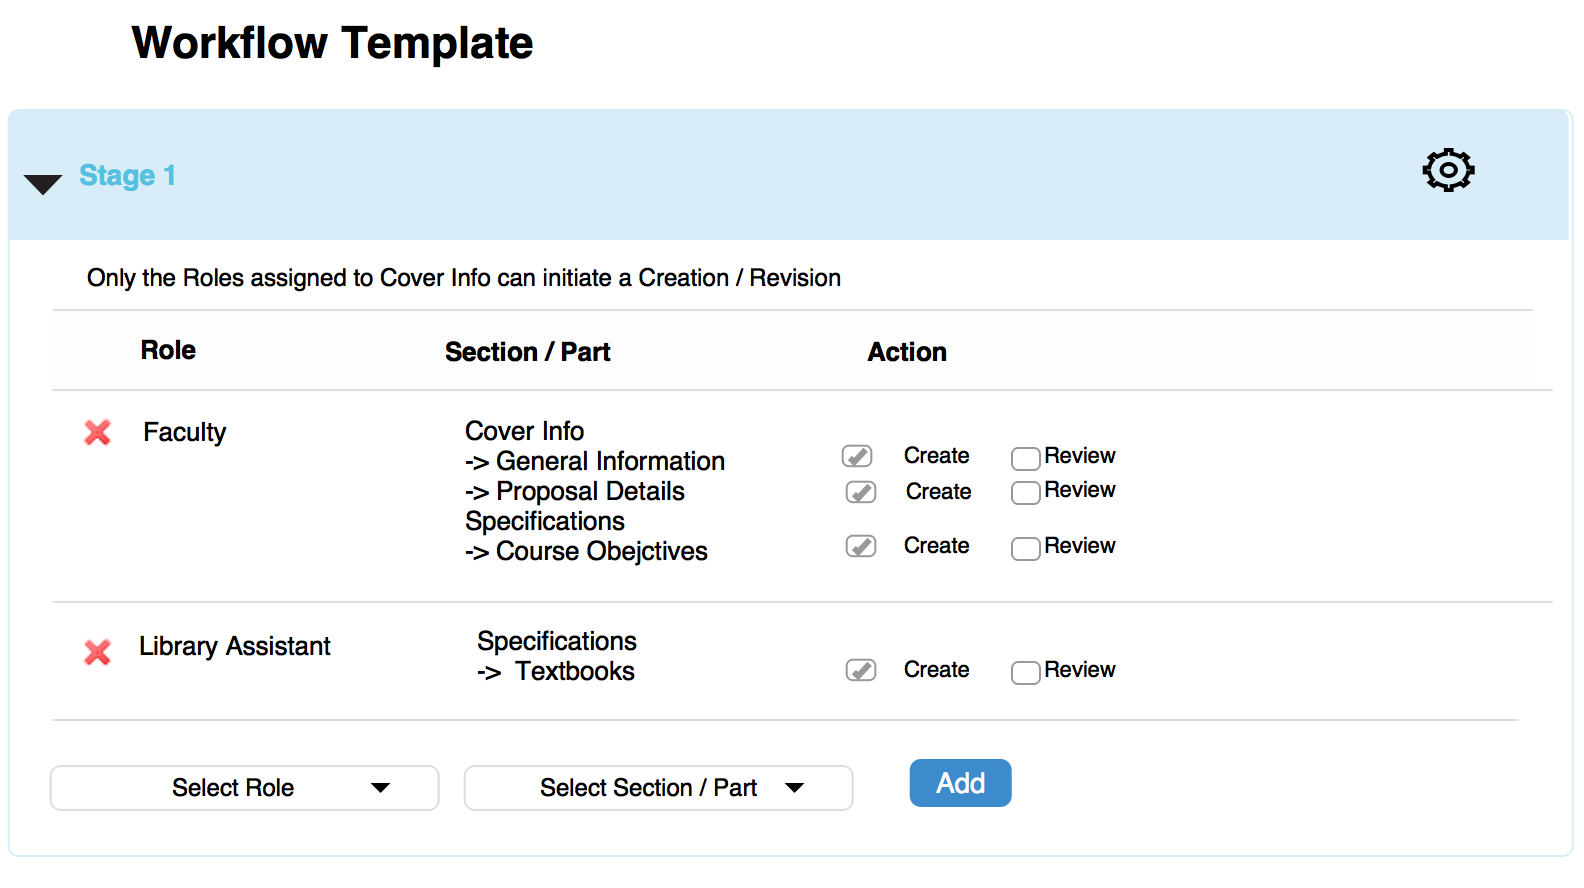
\includegraphics[width=125mm,scale=1]{Capitulos/DesarrollodelaAplicacion/Imagenes/workflow_stage}
\caption{Mockup de la pantalla de plantillas soportando las etapas.}
  \label{workflow_stage}
\end{figure}

\begin{figure}[H]
\centering
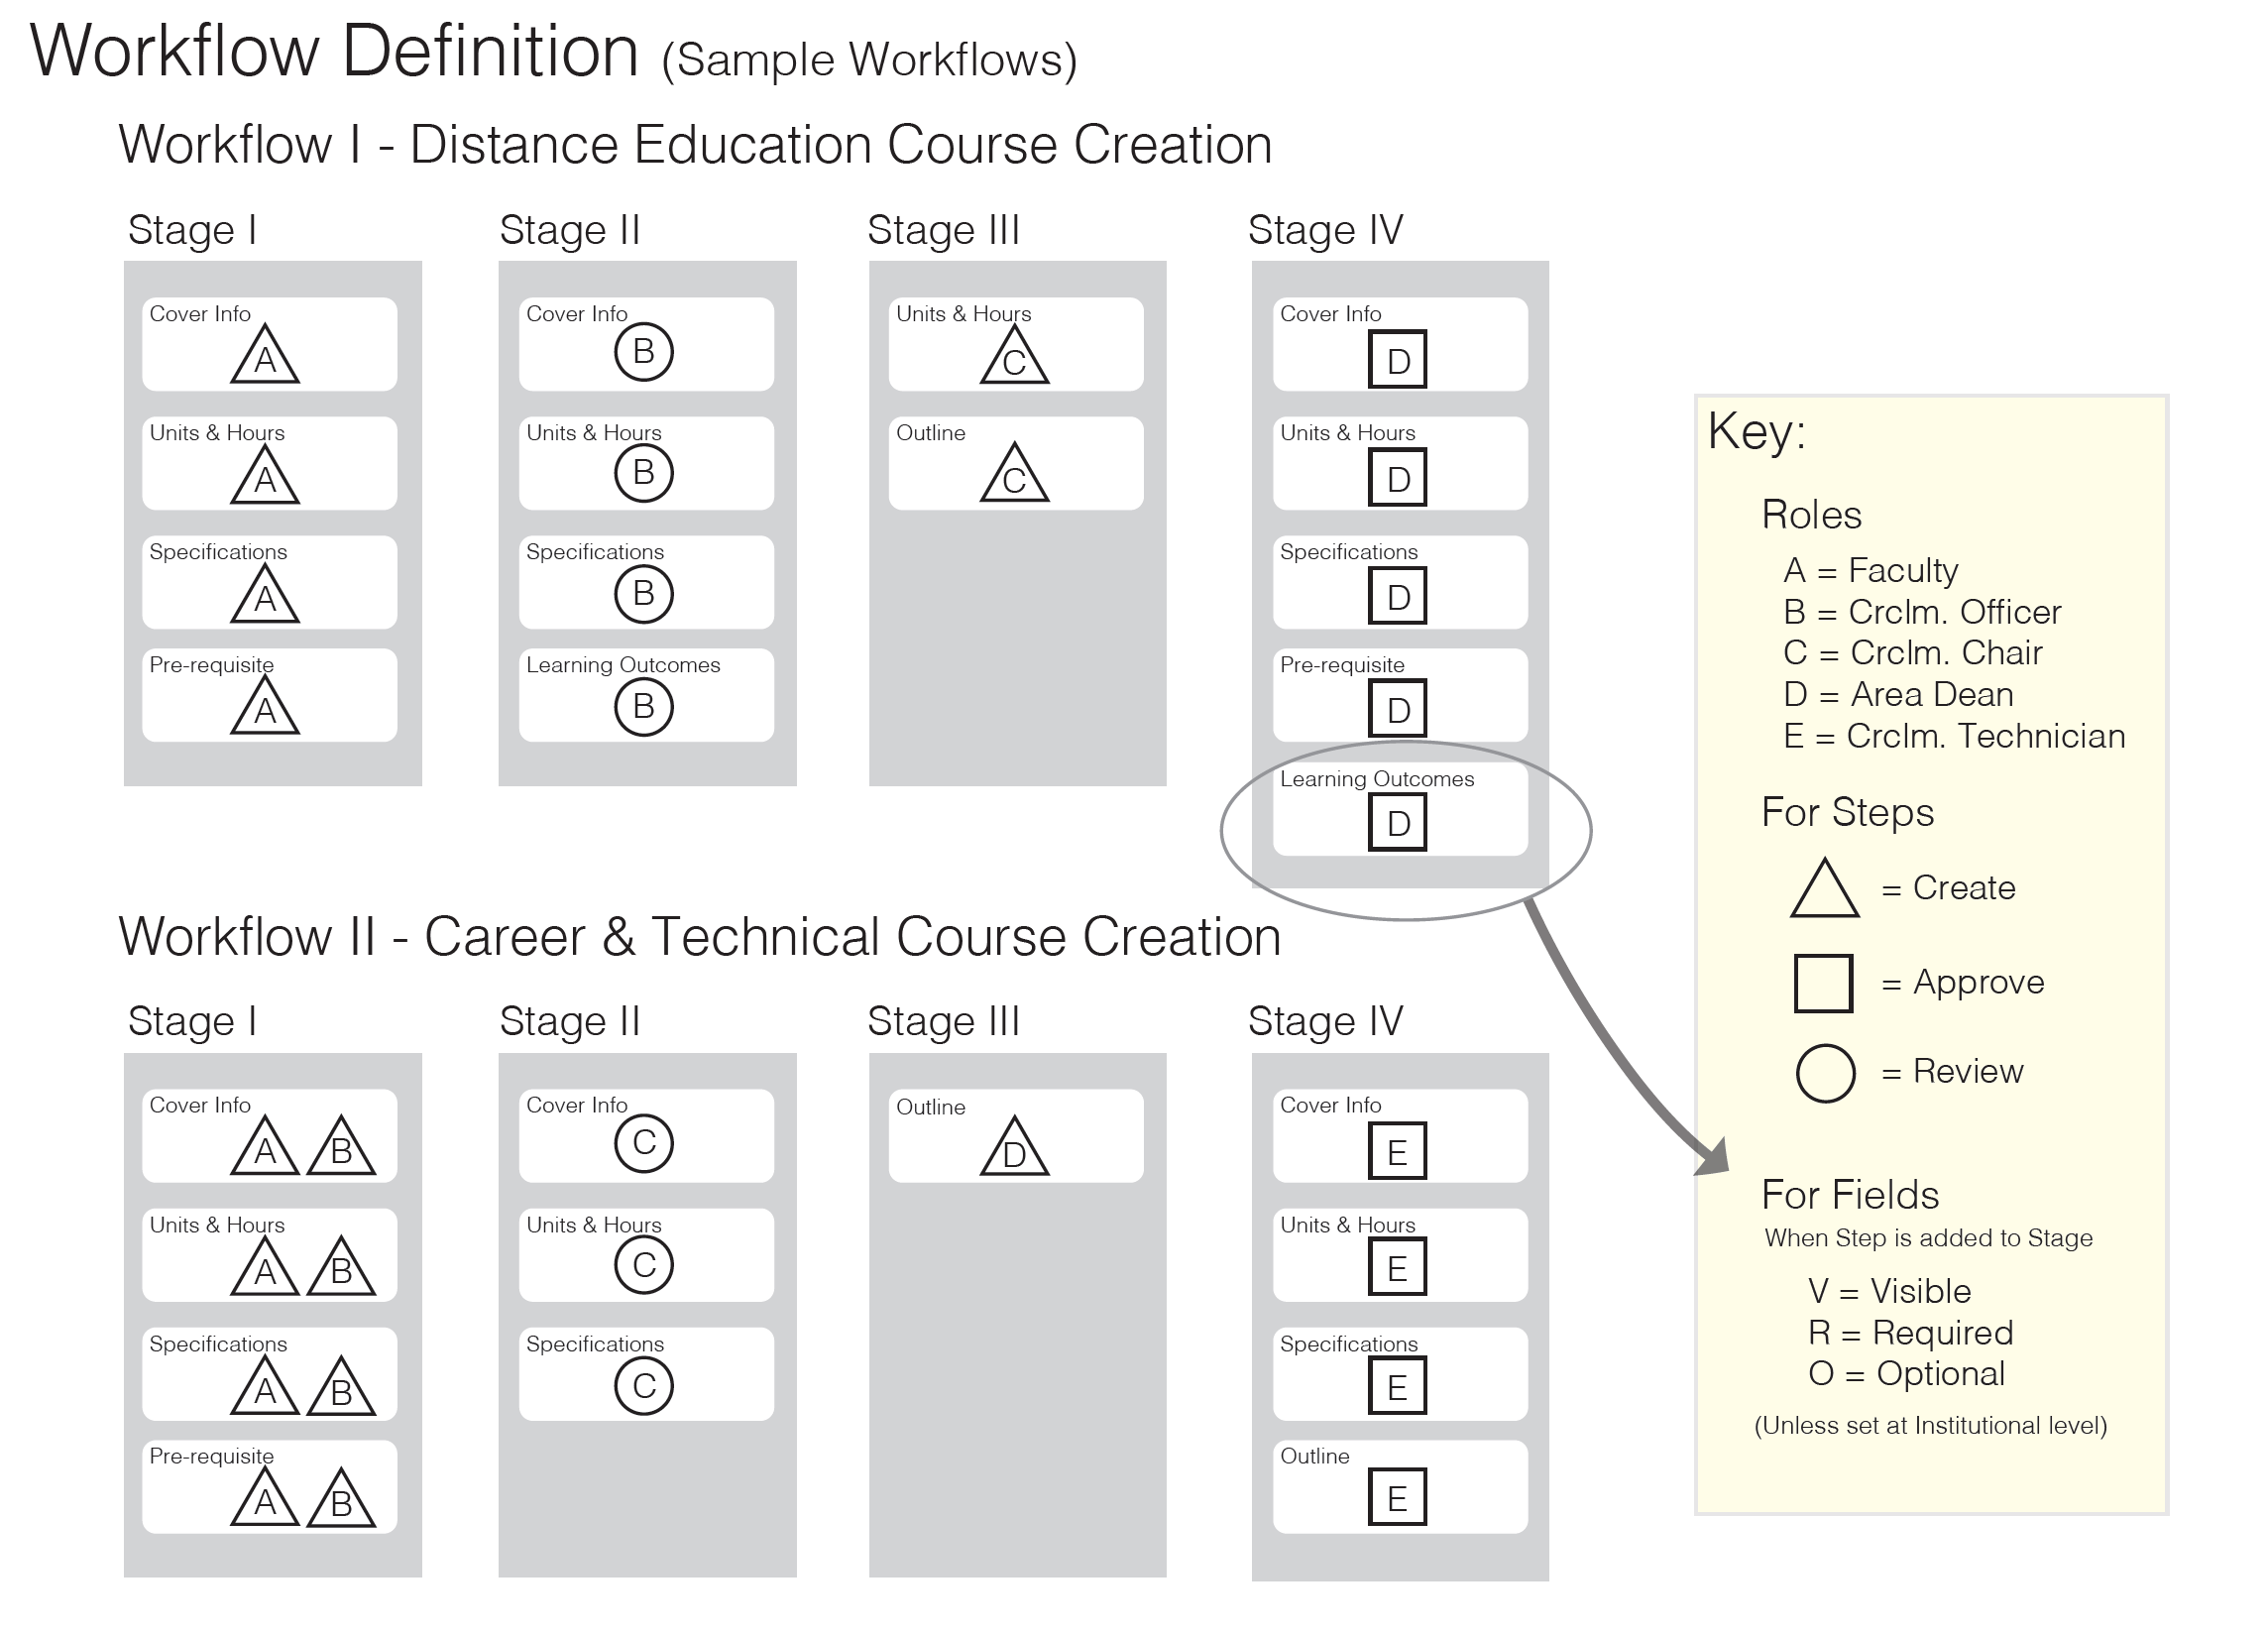
\includegraphics[width=125mm,scale=1]{Capitulos/DesarrollodelaAplicacion/Imagenes/workflow_template_stage}
\caption{Mockup de la pantalla de plantillas con etapas por flujo.}
  \label{workflow_template_stage}
\end{figure}

\subsection{Mejora en comportamientos para las etapas por roles}
La historia de usuario tiene como descripción lo siguiente \enquote{\textit{Como coordinador de educación a distancia, yo solo necesito revisar el esquema del curso para aquellos cursos diseñados para educación a distancia}}.

El criterio de aceptación de la historia consistía en permitir que una etapa que no tiene roles asignados sea opcional.

Algunas de las tareas identificadas en la planificación de las iteraciones eran los siguientes:
\begin{itemize}
	\item Diseñar un plan de pruebas, en estas se identifican las posibles zonas afectadas por la nueva funcionalidad.
	\item Actualizar la pantalla de creación de flujos de trabajo.
	\item Actualizar el mecanismo de transición de etapas.
	\item Mejorar la UI de la vista de etapas de flujos.
\end{itemize}

La historia fue finalizada en tres iteraciones con una cantidad de 108 horas cargadas en el sistema.

\subsection{Composición de etapas y partes}
La historia de usuario tiene como descripción lo siguiente \enquote{\textit{Como presidente curricular, me gustaría ser capaz de componer flujos de trabajo de cursos o programas y etapas (incluyendo actores en cada etapa y sus acciones), para que de esa manera se pueda modelar el proceso curricular en la aplicación}}.

Como criterios de aceptación se encuentran los siguientes:
\begin{itemize}
	\item Cada etapa puede contener una o más partes.
	\item Los actores de cada etapa pueden asignarse actiones a cada parte, o a todas.
	\item Etapas equivalentes no pueden bloquearse entre sí. Por ejemplo, si Suzy y Joe son evaluadores de tres partes, Joe no tiene que esperar que Suzy revise la parte 1 antes de que el pueda evaluar la parte 2, es decir, ambos pueden evaluar sus partes en simultáneo.
\end{itemize}

Algunas de las tareas identificadas en la planificación de las iteraciones eran los siguientes:
\begin{itemize}
	\item Diseño de mockups para su aprobación previa al desarrollo.
	\item Diseño e implementación del modelo de datos que soporte la nueva funcionalidad.
	\item Actualizar las plantillas de flujos de trabajo.
	\item Actualizar los flujos de trabajo de cursos y programas.
	\item Actualizar el sistema de notificaciones.
\end{itemize}

La historia fue finalizada en tres iteraciones con una cantidad de 391 horas cargadas en el sistema.

\subsection{Etapas y partes opcionales en la revisión del flujo}
La historia de usuario tiene como descripción lo siguiente \enquote{\textit{Como administrador curricular quiero ser capaz de configurar mi plantilla de flujo de trabajo para que pueda dividir en etapas donde se especifiquen que roles pueden completar que funciona en una o múltiples secciones o partes de mi programa o curso}}.

Como criterios de aceptación se encuentran los siguientes:
\begin{itemize}
	\item Los roles pueden ser configurados para la acción de creación o revisar, o ambos.
	\item El rol de creación lleva el nombre de creador y para la revisión lleva el nombre de evaluador.
\end{itemize}

Algunas de las tareas identificadas en la planificación de las iteraciones eran los siguientes:
\begin{itemize}
	\item Diseñar un plan de pruebas, en estas se identifican las posibles zonas afectadas por la nueva funcionalidad.
	\item Actualizar la pantalla de creación de flujos de trabajo.
	\item Actualizar el mecanismo de transición de etapas.
\end{itemize}

La historia fue finalizada en tres iteraciones con una cantidad de 76 horas cargadas en el sistema.
\section{Reportes y notificaciones para flujos de trabajo}
\begin{table}[H]
\centering
\caption{Historias de usuario para los reportes y notificaciones de versiones de cursos}
\label{epic:9}
\resizebox{\columnwidth}{!}{%
\begin{tabular}{@{}lllll@{}}
\toprule
Historias de usuario                     			& HE & HC & PH & Sprints \\ \midrule
Notificaciones para las partes del flujo de trabajo & 58 & 60 &  5 &  1 \\
Reporte de esquemas de curso 						& 88 & 91 &  8 &  2 \\ \bottomrule
\end{tabular}
}
\end{table}

\subsection{Notificaciones para las partes del flujo de trabajo}
La historia de usuario tiene como descripción lo siguiente \enquote{\textit{Como especialista curricular, me gustaría que mi equipo de diseño y revisión de flujos de trabajo reciban las notificaciones cuando tengan trabajos pendientes (y alertas cuando este retrasado), para que pueda manejar mejor mis procesos curriculares}}.

Como criterios de aceptación se encuentran los siguientes:
\begin{itemize}
	\item Establecer notificaciones cuando las partes del flujo de trabajo son asignadas a los roles de las personas.
	\item Establecer notificaciones de alerta a asignaciones de partes y etapas. Por ejemplo, 5 días después de su asignación.
	\item Mandar notificaciones por mail.
\end{itemize}

Algunas de las tareas identificadas en la planificación de las iteraciones eran los siguientes:
\begin{itemize}
	\item Diseñar e implementar nuevos modelos de datos que permitan soportar el uso de roles para creadores y editores de partes.
	\item Actualizar el sistema de notificaciones del AMS.
	\item Diseñar e implementar la página de configuración de notificaciones.
\end{itemize}

La historia fue finalizada en tres iteraciones con una cantidad de 60 horas cargadas en el sistema.

\subsection{Reporte de esquemas de curso}
La historia de usuario tiene como descripción lo siguiente \enquote{\textit{Como especialista curricular, me gustaría ser capaz de hacer reportes de registro de esquemas de curso, para que pueda de esta manera ser compartidas por los diferentes colaboradores}}.

Como criterios de aceptación se encuentran los siguientes:
\begin{itemize}
	\item Reporte diseñado por el equipo de diseño curricular.
	\item Incluir competencias es opcional para el reporte.
	\item Incluir alineación de competencias es opcional para el reporte.
	\item Formatos en DOC, PDF o HTML (no Excel).
	\item Se puede ejecutar desde la lista de cursos o de la lista de reportes.
	\item Cuando se corre desde la lista de reportes se pueden elegir uno o más cursos.
\end{itemize}

Algunas de las tareas identificadas en la planificación de las iteraciones eran los siguientes:
\begin{itemize}
	\item Diseñar e implementar el reporte.
	\item Implementar los métodos que acceden a la base de datos.
	\item Diseñar e implementar la página de generación de reportes.
\end{itemize}

La historia fue finalizada en tres iteraciones con una cantidad de 111 horas cargadas en el sistema.
\section{Soporte de versionamiento en el AMS}
\begin{table}[H]
\centering
\caption{Historias de usuario para soporte de versionamiento en el AMS}
\label{epic:10}
\resizebox{\columnwidth}{!}{%
\begin{tabular}{lllll}
\hline
Historias de usuario                                                           & HE & HC & PH & Sprints \\ \hline
Interfaz de alineación de códigos TOP/CIP                                      & 32 & 36 &  3 &  1 \\ 
Renombrar/Reorganizar pestañas para una mejor apariencia del módulo curricular & 32 & 44 &  3 &  1 \\
Lista curricular mejorada para cursos y programas                              &132 &135 &  8 &  2 \\ \hline
\end{tabular}
}
\end{table}

\subsection{Interfaz de alineación de códigos TOP/CIP}
La historia de usuario tiene como descripción lo siguiente \enquote{\textit{Como encargado del sistema de gestión de evaluaciones, me gustaría ser capaz de mantener alineados los codigos TOP a los códigos federales CIP y de esta manera no tener que depender de los administradores para manejar o interpretar estos datos}}.

Como criterios de aceptación se encuentran los siguientes:
\begin{itemize}
	\item Diseñar e implementar una página CRUD para códigos TOP/CIP.
	\item Permitir alinear los códigos.
\end{itemize}

Algunas de las tareas identificadas en la planificación de las iteraciones eran los siguientes:
\begin{itemize}
	\item Diseñar mockups para la nueva página.
	\item Diseñar e implementar el modelo de datos que soporte la funcionalidad.
	\item Desarrollar la página y los métodos de guardado.
\end{itemize}

La historia fue finalizada en una iteración con una cantidad de 36 horas cargadas en el sistema.

\subsection{Reorganización de pestañas para una mejor apariencia del módulo curricular}
La historia de usuario tiene como descripción lo siguiente \enquote{\textit{Como presidente del comité curricular, me gustaría ver las pestañas que están enfocadas a mi trabajo para que pueda navegar y manejar mi tiempo en la aplicación}}.

Como criterios de aceptación se encuentran los siguientes:
\begin{itemize}
	\item Crear pestaña curricular.
	\item Identificar y esconder pestañas no relevantes para el rol.
\end{itemize}

Algunas de las tareas identificadas en la planificación de las iteraciones eran los siguientes:
\begin{itemize}
	\item Diseño de pestañas.
	\item Implementación de pestañas y modificaciones de espacio.
\end{itemize}

La historia fue finalizada en una iteración con una cantidad de 44 horas cargadas en el sistema.


\subsection{Lista curricular mejorada para cursos y programas}
La historia de usuario tiene como descripción lo siguiente \enquote{\textit{Como presidente curricular o miembro del plantel de profesores, me gustaría ser capaz de ordenar/filtrar/visualizar mis cursos y programas, para que de esta manera pueda ver que es importante para mi para luego tomar la acción correspondiente desde esta vista y mi trabajo pueda ser realizado de manera eficiente y con buena visibilidad}}.

Como criterios de aceptación se encuentran los siguientes:
\begin{itemize}
	\item Filtrar por estado de flujo de trabajo, fecha de inicio, fecha de fin y otros a ser designados por el equipo de validación.
	\item Ser capaz de tomar acciones desde la lista (mirar reporte de esquema, empezar una revisión, iniciar el flujo, otros).
	\item Columnas configurables para la vista (resultados de curso, semestre inicial, estado de flujo de trabajo, perfomance de competencia, etc.).
\end{itemize}

Algunas de las tareas identificadas en la planificación de las iteraciones eran los siguientes:
\begin{itemize}
	\item Diseñar mockups para la nueva página.
	\item Diseñar e implementar el modelo de datos que soporte la funcionalidad.
	\item Implementar los filtros.
	\item Implementar página para las columnas configurables.
	\item Actualizar lista.
	\item Actualizar el reporte de esquema de cursos para que soporte múltiples cursos.
\end{itemize}

La historia fue finalizada en dos iteraciones con una cantidad de 135 horas cargadas en el sistema.
\section{Retoques finales}
\subsection{Retoques finales para el flujo de trabajo de cursos}
La historia de usuario tiene como descripción lo siguiente \enquote{\textit{Como especialista curricular, me gustaría poder visualizar y editar todos los campos requeridos por el PCAH}}.

Como criterios de aceptación se encuentran los siguientes:
\begin{itemize}
	\item El flujo de trabajo soporta todos los campos del PCAH.
	\item El flujo de trabajo soporta los campos almacenados adicionales.
\end{itemize}

Algunas de las tareas identificadas en la planificación de las iteraciones eran los siguientes:
\begin{itemize}
	\item Diseñar mockups para todas las partes del flujo de trabajo.
	\item Actualizar las pantallas de las partes del flujo de trabajo.
	\item Actualizar los procedimientos de guardado y versionamiento de entidades.
\end{itemize}

La historia fue finalizada en tres iteraciones con una cantidad de 162 horas cargadas en el sistema.
\section{Aporte}
En la tabla \ref{mis-aportes} se puede apreciar cuáles son los aportes en cada historia de usuario utilizada para desarrollar de manera iterativa el módulo curricular del AMS, los datos fueron calculados desde la herramienta \enquote{JIRA} en la que se cargaban las horas, historias de usuario y fallas del sistema.

En la cual el trabajo consistía en desarrollo de la historia, desarrollo de tests, y la persona que no desarrolló la historia es la encargada de hacer la validación de código y funcionalidad.

\begin{table}[H]
\centering
\caption{Tabla de historias de usuario y aportes}
\label{mis-aportes}
\begin{tabular}{@{}ll@{}}
\toprule
Historias de usuario                                & Aporte \\ \midrule
Diseño de modelo de versionamiento de entidades     &  20\%  \\
Versionamiento de competencias                      & 61,5\% \\
Flujo de trabajo simple                             & 62,5\% \\
Aprobar pasos completados de flujos de trabajo      &  40\%  \\
Rechazar pasos completados de flujo de trabajo      &  60\%  \\
Buzón de entradas de flujos de trabajo              &  40\%  \\
Notificaciones con soporte a etapas                 &  20\%  \\
Versionamiento de evaluaciones                      & 37,5\% \\
Versionamiento de cursos                            & 61,5\% \\
Información básica de curso                         &  20\%  \\
Horas y unidades de evaluación de curso             &   8\%  \\
Especificaciones de curso                           &  40\%  \\
Requisitos de cursos                                &  60\%  \\
Revisar y aprobar curso                             &  40\%  \\
Competencias de curso                               &  25\%  \\
Esquema de curso                                    &  20\%  \\
Códigos de clasificación de curso                   &  60\%  \\
Información básica del programa                     &  50\%  \\
Competencias de programa                            &  60\%  \\
Bloques de curso por programa                       &  20\%  \\
Visualizar cambios en los campos                    &   8\%  \\
Roles de creación y edición para partes             &  23\%  \\
Diseño e implementación de etapas                   &  38\%  \\
Mejora en comportamientos para las etapas por roles & 37,5\% \\
Composición de etapas por roles                     &  23\%  \\
Etapas y partes opcionales por en la revisión       & 37,5\% \\
Notificaciones para las partes de flujos de trabajo &  20\%  \\
Reporte de esquemas de curso                        &  25\%  \\
Interfaz de alineación de códigos TOP/CIP           & 100\%  \\
Reorganización de pestañas del módulo curricular    & 100\%  \\
Lista mejorada de cursos y programas                & 100\%  \\
Retoques finales para el flujo de trabajo de curso  & 37,5\% \\ \bottomrule
\end{tabular}
\end{table}

Dichas historias de usuario eran entregadas para validación de parte del equipo de desarrolladores y por el equipo de expertos en didáctica, una vez que era aprobada se procedía a integrar el nuevo código con el del AMS. Si en la aplicación o en el módulo se encontraban fallas, se procedían a crear tickets de fallas. Además, si habían mejoras que hacerse se creaban tickets de mejoras. En la figura \ref{tickets_by_type} podemos ver la distribución de tickets aportados por tipo.

\begin{figure}[H]
\centering
\begin{tikzpicture}
	\pie [rotate = 180] {45/Historias de usuario, 48.3/Fallas, 6.7/Mejoras}
\end{tikzpicture}
\caption{Distribución de tickets por tipo.}
  \label{tickets_by_type}
\end{figure}

Las historias de usuario que no cumplieron con todos los criterios de aceptación vuelve a ser abierta para que se continue su desarrollo. El porcentaje de historias que no cumplieron los criterios de aceptación se puede apreciar en la figura \ref{user_story_perc}.

\begin{figure}[H]
\centering
\begin{tikzpicture}
	\pie [rotate = 180] {85.2/Terminada, 14.8/Reabierta}
\end{tikzpicture}
\caption{Porcentajes de historias de usuario reabiertas.}
  \label{user_story_perc}
\end{figure}

Los tickets de fallas que se trabajaron fueron fallas o errores de dominio encontrados en la funcionalidad del módulo curricular, cuando el equipo de desarrollo solucionaba dichas fallas debía seguir el mismo proceso de validación. En caso de que la falla mediante pruebas seguía se volvía a abrir para que se continúe trabajando hasta que cumpla con el criterio de aceptación que era solucionar la falla que se reportaba. En la figura \ref{bugs_perc} se puede ver cuántas fallas fueron cerradas y reabiertas en el periodo de desarrollo.

\begin{figure}[H]
\centering
\begin{tikzpicture}
	\pie [rotate = 180] {86.2/Terminado, 13.8/Reabierto}
\end{tikzpicture}
\caption{Porcentajes de tickets de fallas que fueron reabiertos.}
  \label{bugs_perc}
\end{figure}

Los tickets de fallas por lo general eran tickets de dificultad pequeña que un programador podía terminar en uno o dos días aproximadamente, es decir en un sprint. En cambio, las historias de usuario eran de mayor dificultad y podía tomar a varios desarrolladores hasta más tiempo que sprint podía brindar, en esos casos se continuaba en el siguiente sprint o se separaba la funcionalidad en tickets más pequeños, como se puede apreciar en la figura \ref{sprint_perc}.

\pgfplotstableread[row sep=\\,col sep=&]{
    interval 		& carT \\
    1 sprint     	& 22  \\
    2 sprints     	& 5 \\
    3 sprints    	& 4 \\
    4 sprints   	& 1 \\
    }\mydata

\begin{figure}[H]
\centering
\begin{tikzpicture}
    \begin{axis}[
            ybar,
            symbolic x coords={1 sprint,2 sprints, 3 sprints, 4 sprints},
            xtick=data,
            nodes near coords,
        ]
        \addplot table[x=interval,y=carT]{\mydata};
        \legend{Historias de usuario}
    \end{axis}
\end{tikzpicture}
\caption{Cantidad de historias de usuarios terminadas en cantidad de sprints.}
  \label{sprint_perc}
\end{figure}

\section{Sumario}
Se han expuesto las épicas e historias de usuarios desarrolladas durante el periodo de programación del módulo curricular, donde las funcionalidades de las mismas son definidas como criterios de aceptación. El PO define las historias con una descripción que sigue la definición de la metodología Ágil buscando valor de negocio para el usuario final. 

Cada historia de usuario estaba compuesta de tareas, las mismas permitían a los desarrolladores la división de trabajo pendiente. Cada tarea es asignada a un usuario como responsable, pero varias personas podrían trabajar en la misma tarea en conjunto, que era lo que generalmente pasaba para agilizar el desarrollo.

Y, por último, se colocan los aportes realizados por historia de usuario durante el caso de estudio, dichos porcentajes son calculados por la herramienta que utiliza la organización para la gestión de proyectos.

% VALIDACION
% Chapter 7

\chapter{Validación del desarrollo} \label{capitulo7}

El flujo de validación de las historias de usuario es un proceso preciso, consistente y controlado por parte de los desarrolladores y de los miembros del equipo educativo. Entre las validaciones se encuentran las siguientes:
\begin{itemize}
	\item Entradas, salidas y funciones del módulo curricular.
	\item Todos los requisitos no funcionales con sus respectivas pruebas. Entre ellas están las pruebas de rendimiento, fiabilidad, precisión y tiempos de respuesta.
	\item Interacciones de usuario.
	\item Funcionamiento en diferentes arquitecturas (plataformas, sistemas operativos, navegadores, etc.).
	\item Límites de intervalos, valores por defecto y valores específicos que el módulo acepta.
	\item Criterios de aceptación, especificaciones en los requerimientos, funcionalidades, o funciones implementadas en el software.
\end{itemize}

Sin embargo, vale la pena resaltar, el hecho de que se redacta un documento de este tipo no nos obliga a que todo el proceso sea documentado. De hecho, para la metodología ágil, se puede desarrollar de forma incremental. Pero antes de cualquier lanzamiento a los usuarios, se hacen varias validaciones de funcionamiento para cerciorarse de que refleja absolutamente correctamente el estado atual del comportamiento del sistema de software a partir de ese momento. Es un trabajo de gran magnitud, pero no exige que se lo haga de una vez, y de antemano.

El objetivo de cada sprint ágil es producir un producto utilizable, y, como la metodología ágil se desarrolló como un modelo para su uso en el desarrollo de software, más a menudo el producto utilizable es el código. La verificación del trabajo realizado en cada sprint tiene tres partes: pruebas automatizadas, revisión por pares y revisión del propietario del producto o en nuestro caso por parte del equipo educativo.

\section{Pruebas automatizadas}
Por pruebas automatizadas nos referimos por funcionalidades programas para realizar la mayoria de las pruebas de código que debe hacer el desarrollador. Con las pruebas automatizadas, el equipo de desarrollo puede desarrollar y probar su código de manera rápida, la cual es un gran beneficio para los proyectos ágiles.

A menudo, el equipo de desarrollo desarrolla el código durante el día y corren las pruebas automatizadas durante la noche para tener los resultados a la mañana. Por la mañana, el equipo del proyecto puede revisar el informe de errores que generó el programa de pruebas, informar sobre cualquier problema durante el informe diario de cada desarrollador y buscar corregir esos problemas inmediatamente durante el día.

Algunas de las pruebas automatizadas pueden incluir:
\begin{itemize}
	\item \textbf{Unit Testing:} pruebas automatizadas de pequeñas funcionalidades de código, a nivel de componentes.
	\item \textbf{System Testing:} pruebas automatizadas de código integradas con el sistema.
	\item \textbf{Static Testing:} pruebas estáticas que verifican que el código cumple con los estándares basadas en reglas y buenas prácticas que el equipo de desarrollo estableció al inicio del proyecto.
\end{itemize}

\section{Revisión por pares}
Revisión por pares significa que los miembros del equipo de desarrollo revisa el código del otro miembro.

El equipo de desarrollo puede realizar evaluaciones por pares durante el desarrollo. La forma en que están sentados puede facilitar este proceso ya que puede dirigirse a la persona que está a su lado y pedirle que revise su trabajo. El equipo de desarrollo también puede reservar tiempo durante el día específicamente para revisar el código. Los equipos autogestionarios deben decidir qué es lo que funciona mejor para su equipo ya sea al inicio de cada iteración o luego de cierto periodo de pruebas.

\section{Revisión por parte del equipo de validación}
Una vez finalizado el proceso de desarrollo y verificación de las historias de usuario, el equipo de validación se encarga de revisar la funcionalidad y verifica que cumple con los criterias de aceptación. El equipo de validación forma parte del ciclo de vida de cada historia de usuario y hace las verificaciones acorde se agreguen a su lista de trabajos pendientes.

Finalmente, el propietario del producto debe comprobar y verificar que la historia de usuario en cuestión cumple con la definición de \enquote{DONE}. Cuando una historia de usuario cumple la definición de \enquote{DONE}, el propietario del producto actualiza la tabla de tareas moviendo la historia de usuario de la columna \enquote{UNDER REVIEW} a la columna \enquote{DONE}.

\section{Revisión por parte del cliente}
El papel del cliente es más notorio en el proceso de desarrollo de las metodologías ágiles; uno de los principios del Manifiesto dice que los responsables de negocio y los desarrolladores trabajan juntos de manera cotidiana durante todo el proyecto [6]. Esta condición no es fácil de satisfacer. Los clientes pueden estar separados geográficamente o puede ser muy costoso para ellos mantener un representante con la capacidad de responder por la totalidad de los requerimientos del sistema que se está desarrollando, de manera permanente.
Para resolver estas limitantes es posible utilizar varias estrategias. La primera, tener múltiples dueños de historias de usuario. Con esto se busca no inhabilitar a un cliente durante todo el desarrollo. Al tener cada historia de usuario su dueño, una vez que esta termina, la siguiente se trata como una historia de usuario con un dueño distinto. La segunda estrategia consiste en nombrar un intermediario del cliente, lo que involucra a un desarrollador del equipo que coordina de manera conjunta los requerimientos.

% CONCLUSION
% Chapter 8

\chapter{Conclusión y aportes} \label{capitulo7} 
En este capítulo se encuentran las conclusiones obtenidas, acompañado de un breve resumen de toda la investigación. Se exponen los aportes a la problemática, asi como también se proponen posibles temas de investigación y trabajos futuros o complementarios, que puedan continuar a partir del presente trabajo.

\section{Conclusiones generales}
En el proyecto final se planteó como un caso de estudio con enfoque en la interacción humano-computador a través de una observación participante en el diseño e implementación de un módulo de gestión curricular para un sistema de gestión de evaluaciones basadas en competencias académicas. Se contó con un grupo de expertos en educación así como un grupo de usuarios que acompañaron todo el proceso de desarrollo y validación.

Se diseñó la manera de integrar y estructurar procesos separados de validación de cursos y programas para el estado de California con un sistema de gestión de evaluaciones basadas en competencias. Dicho proceso se realizaba en el pasado en papel y tenía sus falencias debido a que el mismo requería mucho tiempo en revisar y aprobar los formularios pertinentes. Asimismo, la complejidad del flujo aumentaba cuando habían más personas colaboradoras o evaluadoras en el proceso.

Debido a que los requerimientos eran cambiantes y el equipo que diseñaba no disponía de un panorama completo de las funcionalidades del módulo curricular, la elección de la metodología ágil para el desarrollo del proyecto fue acertada debido a que la misma permitía el desarrollo iterativo e incremental del software con validaciones del cliente como proceso de desarrollo, que en este caso el equipo de validación tomaba el rol de cliente debido al conocimiento y experiencia en didáctica de sus miembros.

Por lo tanto, algunas de las experiencias adquiridas en este caso de estudio al utilizar la metodología ágil fueron las siguientes:
\begin{itemize}
	\item Se pudo mejorar rápidamente la elección de que construir, pero tuvimos que tener en cuenta las revisiones de los expertos y usuarios que sugirieron cambios para luego realizarlos.
	\item Se realizó un importante esfuerzo en modular las unidades de trabajo en pequeños incrementos.
	\item Con la experiencia que se fue acumulando, el equipo fue progresivamente mejorando la calidad de sus estimaciones respecto al trabajo que se podía realizar en cada sprint.
\end{itemize}

El diseñar los flujos de trabajo para el diseño y revisión de formularios de competencias, cursos, y programas permitió a los profesores encargados y a los evaluadores de dichos formularios seguir el proceso de una manera intuitiva logrando una mejor experiencia de usuario. Esto se puede apreciar en la aceptación de las historias de usuario y la creación de nuevas historias de mejora, propuestas por los usuarios, que a su vez fueron aprobadas. Un ejemplo de estas mejoras fue la generación de mensajes en cada paso para que el usuario pueda acceder en su buzón de entrada en caso de que tuviera trabajo pendiente.

En el desarrollo del módulo se utilizaron muchas de las tecnologías y herramientas que disponía el sistema como requerimiento no funcional de parte de la organización. El uso de estas tablas en común para la funcionalidad de plantillas de flujos de trabajo trajo consigo muchos problemas técnicos, debido a que agregaba complejidad a las mismas y además las pruebas de componentes se convertían en pruebas de regresión debido a la complejidad de la estructura. 

La decisión de utilizar MySQL para guardar el flujo de trabajo y todos sus datos temporales también acarreó muchos problemas técnicos pues la funcionalidad y el estándar de estructuras de datos de cursos tienen cambios constantes. Sin embargo, la naturaleza iterativa del proceso de desarrollo ágil nos permitió identificar estas falencias y corregirlas en el curso del proyecto.

Debido a la capa adicional de comunicaciones con el usuario final personificada por el equipo de Estados Unidos (que en nuestro caso actúa como cliente), la realimentación de valor real o valor aún necesario provisto al usuario final es lenta e implica grandes cambios luego de varios sprints. Sin embargo, dado el gran número de usuarios finales involucrados, el grupo de expertos también ayudó a clasificar y organizar la comunicación con los mismos.

A pesar de todas las falencias de desarrollo, el módulo tuvo resultados positivos por parte de los usuarios finales ya que la herramienta construida automatiza trabajos de validación curricular para las instituciones. Además, al tener comentarios acerca de qué habría que mejorar en la aplicación y con la utilización de la metodología ágil se permitió que se creen nuevas historias de usuario para algunos retoques futuros en el módulo curricular. 

\section{Aportes del proyecto}
La capacidad otorgada por este sistema para gestionar el diseño y validación de material curricular en el estado de California, y la comunicación que ofrece entre los encargados del diseño de los formularios y los evaluadores de los mismos constituye el principal aporte de este trabajo.

Además, podemos citar otros aportes:
\begin{itemize}
	\item El módulo desarrollado reemplaza la preparación manual de formularios, los procesos de revisión y aprobación curricular de colegios ya sea para universidades, cursos, y programas.
	\item El módulo constituye un ambiente que puede ser accedido desde cualquier navegador y la capacidad de compartir comentarios, permite a las personas trabajar en conjunto sin necesidad de agendar reuniones para desarrollar el formulario o las revisiones.
	\item El módulo desarrollado permite almacenar los datos nuevos, históricos, propuestos y activos de competencias, cursos, y programas.
	\item Al proveer notificaciones automatizadas cuando hay cambios de estado en los flujos de trabajo.
	\item En la opinión de expertos y usuarios, la utilización del módulo desarrollado reduciría el tiempo promedio de formulación y revisión de cada flujo de diseño e implementación de flujos de trabajo, debido a que el mismo facilita la labor de llenar formularios utilizando información ya existente en el AMS.
\end{itemize}

\section{Proyectos futuros}
En consenso con los usuarios finales de la aplicación y los que diseñan las historias de usuarios se observaron ciertas características que podrían dar una mayor utilidad al proyecto, donde citaremos algunos de los trabajos futuros ya creadas como épicas del proyecto:
\begin{itemize}
	\item \textbf{Importador de cursos:} muchos de los cursos que ya fueron agregados al sistema de gestión curricular del estado de California existen y como trabajo futuro para el módulo curricular es la forma de importar todos estos cursos al AMS sin necesidad de hacer todo el flujo de trabajo para las competencias, cursos y programas válidos actualmente.
	\item \textbf{Migración de motor de base de datos de los flujos de trabajo:} como ya comentamos, la decisión de tecnología en cuanto al motor de base de datos fue una decisión errónea, debido a que el estándar de California para diseño y revisión de cursos y programas puede variar con el tiempo y la utilización de MySQL como motor de base de datos dificulta el desarrollo en sí debido al constante cambio del modelo de datos, por lo que se considera un motor de base de datos no relacional basada en documentos, e.g. \enquote{MongoDB} como una opción a futuro.
	\item \textbf{Acceso de información a través de API\footnote{de sus siglas en inglés, Application Programming Interface, que sirve como un conjunto de reglas para que las aplicaciones puedan comunicarse entre ellas.} pública:} es una práctica que exige el estado de California que todos los datos en cuanto a cursos y programas de las universidades puedan ser accedidas desde una API pública. Por lo tanto, se debe diseñar e implementar una interfaz pública que permita comunicarse y acceder a los datos del módulo curricular.
	\item \textbf{Catálogo de cursos:} los CMS del estado tienen la opción de mostrar sus cursos válidos de manera pública para que las universidades puedan cargar en sus sistemas académicos como se aprecia en la figura \ref{after_creation}. Por lo tanto, como trabajo futuro para el módulo curricular se busca catalogar los cursos de manera pública desde una interfaz web.
	\item \textbf{Flujo de trabajo para evaluaciones:} el mismo flujo de trabajo que se diseño e implementó para las competencias, cursos, y programas, se debe implementar para las evaluaciones.
\end{itemize}
Desde el punto de vista académico sería interesante realizar una experiencia controlada de usabilidad del sistema para medir con mayor precisión las ganancias en materia de productividad que conlleva la utilización de este módulo.

%----------------------------------------------------------------------------------------
%	THESIS CONTENT - APPENDICES
%----------------------------------------------------------------------------------------

%\appendix % Cue to tell LaTeX that the following "chapters" are Appendices

% Include the appendices of the thesis as separate files from the Appendices folder

%% Appendix A

\chapter{Appendix Title Here} % Main appendix title

\label{AppendixA} % For referencing this appendix elsewhere, use \ref{AppendixA}

Write your Appendix content here.
%\include{Apendices/AppendixB}
%\include{Apendices/AppendixC}

%----------------------------------------------------------------------------------------
%	BIBLIOGRAPHY
%----------------------------------------------------------------------------------------

\renewcommand{\bibname}{Bibliografía}

\printbibliography[heading=bibintoc]

%----------------------------------------------------------------------------------------

\end{document}
